\documentclass[11pt,a4paper]{article}
\usepackage[utf8]{inputenc}
\usepackage[T1]{fontenc}
\usepackage{lmodern}
\usepackage[spanish]{babel}
\AtBeginDocument{\shorthandoff{"}}
\usepackage{geometry}
\geometry{left=2.2cm,right=2.2cm,top=2.2cm,bottom=2.2cm}
\usepackage{graphicx}
\usepackage{longtable}
\usepackage{booktabs}
\usepackage[table]{xcolor}
\definecolor{UTECblue}{HTML}{1F4E79}
\usepackage{caption}
\usepackage{float}
\usepackage{listings}
\lstset{basicstyle=\ttfamily\small,breaklines=true,frame=single,backgroundcolor=\color{gray!8}}
\usepackage{enumitem}
\usepackage{amssymb}
\usepackage{fancyhdr}
\usepackage{hyperref}
\hypersetup{colorlinks=true,linkcolor=UTECblue,urlcolor=UTECblue,breaklinks=true}
\graphicspath{{./}{./evidencias/}{evidencias/}}
\pagestyle{fancy}
\fancyhead[L]{\small Informe T\'ecnico VyV --- Sistema de Calificaciones UTEQ}
\fancyhead[R]{\small \thepage}
\fancyfoot[C]{}
\setlength{\headheight}{14pt}
\begin{document}

\begin{titlepage}
\centering
{\Large UNIVERSIDAD T\'ECNICA ESTATAL DE QUEVEDO\par}
{\large Facultad de Ciencias de la Computaci\'on --- Ingenier\'ia en Software\par}
\vspace{1.5cm}
{\Large\bfseries Sistema de Registro de Calificaciones\par}
{\large Documento T\'ecnico de Verificaci\'on y Validaci\'on de Software\par}
\vspace{1.5cm}
\begin{tabular}{rl}
Materia: & Verificaci\'on y Validaci\'on de Software \\
Integrantes: & Castro Espinoza Kevin Mois\'es $\cdot$ V\'elez L\'opez Ricardo El\'ias $\cdot$ Panama Murillo Moises Antonio \\
Docente: & Ing.\ Cordero Bazurto Jos\'e Steven \\
Fecha: & Septiembre 2026 \\
Versi\'on: & 1.0 \\
\end{tabular}
\vfill
{\large Quevedo --- Ecuador\par}
\end{titlepage}
\pagenumbering{roman}
\tableofcontents
\newpage
\pagenumbering{arabic}


\hrule\vspace{0.4em}


\section*{Índice general}
\addcontentsline{toc}{section}{Índice general}


\begin{enumerate}[leftmargin=*]
\item Presentación del proyecto y marco teórico
\item Metodología y plan de pruebas
\item Técnica Personas
\item Historias de usuario y criterios de aceptación
\item Casos de prueba manuales
\item Automatización de pruebas (API y UI)
\item Casos de prueba de aceptación del usuario (UAT)
\item Prueba de la versión Beta
\item Registro de observaciones de la Beta
\item Encuesta de satisfacción
\item Métricas del proceso de V\&V
\item Resumen de hallazgos y correcciones
\item Conclusiones y recomendaciones
\item Anexos
\end{enumerate}


\textbf{Índice de figuras}


\begin{itemize}[leftmargin=*]
\item Figura 1. Arquitectura en tres capas del sistema.
\item Figura 2. Perfil de los encuestados (N = 89).
\item Figura 3. Satisfacción por pregunta (Bloque A, Likert 1--5).
\item Figura 4. Resultados del Bloque B (Sí/No).
\item Figura 5. Métricas de ejecución de casos de prueba.
\item Figuras 6--14. Capturas de pantalla de los casos de prueba manuales (CP-01, CP-02, CP-04, CP-05, CP-08, CP-10, CP-11, CP-13 y CP-14).
\item Figuras 15--21b. Análisis por módulo: login, estudiantes, calificaciones, consulta del representante, reportes, auditoría y panel de psicóloga.
\item Figuras 22--28. Capturas de pantalla de los casos UAT-01 a UAT-07.
\end{itemize}


\textbf{Índice de tablas}


\begin{itemize}[leftmargin=*]
\item Tabla 1. Tecnologías por capa del sistema.
\item Tabla 2. Roles y usuarios del sistema.
\item Tabla 3. Personas y su foco de pruebas.
\item Tabla 4. Matriz de trazabilidad historias {$\rightarrow$} pruebas.
\item Tabla 5. Resumen de casos de prueba manuales.
\item Tabla 6. Clasificación de los 66 checks de API.
\item Tabla 7. Distribución de los 35 tests de Playwright.
\item Tabla 8. Categorías de hallazgos de la instalación limpia.
\item Tabla 9. Resumen de casos UAT.
\item Tabla 10. Participantes de la prueba Beta.
\item Tabla 11. Condiciones de la prueba Beta.
\item Tabla 12. Consolidado de observaciones de la Beta.
\item Tabla 13. Perfil de encuestados.
\item Tabla 14. Frecuencias Likert (N = 89).
\item Tabla 15. Bloque B (Sí/No).
\item Tabla 16. Transcripción de respuestas abiertas (P19--P20).
\item Tabla 17. Hallazgos H1--H15 y correcciones.
\item Tabla 18. Métricas del proceso de V\&V.
\end{itemize}


\hrule\vspace{0.4em}


\section*{1. Presentación del proyecto y marco teórico}
\addcontentsline{toc}{section}{1. Presentación del proyecto y marco teórico}


\subsection*{1.1 Problema}
\addcontentsline{toc}{subsection}{1.1 Problema}


En la Unidad Educativa, el registro de calificaciones se realizaba mediante planillas físicas y archivos Excel distribuidos por correo electrónico. Este esquema de trabajo presentaba múltiples limitaciones:


\begin{itemize}[leftmargin=*]
\item \textbf{Pérdida de trazabilidad:} cualquier persona podía corregir una nota a mano sin dejar registro del cambio ni del responsable.
\item \textbf{Demoras en el cálculo de promedios:} los docentes sumaban y promediaban de forma manual, con errores frecuentes de digitación.
\item \textbf{Riesgo de inconsistencia:} coexistían varias versiones de la planilla (una por docente y por parcial), sin un control único de la información.
\item \textbf{Dificultad de acceso para los representantes:} las familias debían acudir físicamente al plantel para conocer las notas de sus hijos.
\item \textbf{Ausencia de control por rol:} cualquier docente podía ver o modificar información ajena, lo que rompía la confidencialidad académica.
\end{itemize}


Por ello se desarrolló un \textbf{sistema web de registro y consulta de calificaciones}, que además debía ser sometido a un proceso formal de \textbf{verificación y validación (V\&V)} antes de su puesta en producción. Este documento describe dicho proceso: las técnicas aplicadas, la instrumentación de las pruebas (manuales, automatizadas y de aceptación), los resultados obtenidos y las correcciones realizadas.


\subsection*{1.2 Objetivos}
\addcontentsline{toc}{subsection}{1.2 Objetivos}


\subsubsection*{Objetivo general}
\addcontentsline{toc}{subsubsection}{Objetivo general}


Verificar y validar el Sistema de Registro de Calificaciones de la Unidad Educativa, garantizando que cumple los requisitos funcionales y de control de acceso definidos y que satisface a los usuarios finales.


\subsubsection*{Objetivos específicos}
\addcontentsline{toc}{subsubsection}{Objetivos específicos}


\begin{enumerate}[leftmargin=*]
\item Aplicar técnicas de verificación estática y dinámica (revisión de código, pruebas de caja negra por API y pruebas end-to-end por interfaz) sobre el repositorio del sistema.
\item Ejecutar un plan de casos de prueba manuales y automatizados alineado a los requisitos del usuario, con evidencia trazable.
\item Realizar pruebas de aceptación (UAT) y una prueba Beta con usuarios finales simulados según la técnica Personas.
\item Medir la satisfacción del usuario mediante una encuesta estructurada de 20 preguntas aplicada a 89 usuarios.
\item Documentar los hallazgos, corregirlos y verificar su cierre, y emitir conclusiones y recomendaciones.
\end{enumerate}


\subsection*{1.3 Alcance y limitaciones}
\addcontentsline{toc}{subsection}{1.3 Alcance y limitaciones}


\subsubsection*{Alcance}
\addcontentsline{toc}{subsubsection}{Alcance}


\begin{itemize}[leftmargin=*]
\item Gestión de estudiantes, materias, cursos, ciclos, parciales, tipos de calificación y periodos académicos.
\item Registro de calificaciones por parte de docentes, con validación de rango 0--10 y autorización por materia asignada.
\item Consulta de notas y promedios para representantes (solo sus hijos) y para estudiantes (solo sus propias notas).
\item Reportes de promedios por periodo y panel de rendimiento académico para psicóloga.
\item Panel de auditoría de cambios (INSERT/UPDATE/DELETE con datos antes/después) y respaldos de base de datos.
\item Control de acceso por roles: administrador, profesor, representante, psicóloga y estudiante.
\end{itemize}


\subsubsection*{Limitaciones}
\addcontentsline{toc}{subsubsection}{Limitaciones}


\begin{itemize}[leftmargin=*]
\item El entorno de pruebas es de laboratorio: el sistema se ejecuta sobre \texttt{localhost} con una base de datos de prueba poblada con datos sintéticos; no se realizaron pruebas de carga masiva sobre infraestructura de producción.
\item La prueba Beta se ejecutó con participantes simulados (basados en la técnica Personas) por razones de confidencialidad y disponibilidad; los datos de la encuesta siguen el mismo criterio de simulación con base en los módulos involucrados.
\item Las pruebas de compatibilidad se limitaron a los navegadores Chrome y Edge en sistemas de escritorio y a la vista móvil sobre dispositivos de prueba.
\end{itemize}


\subsection*{1.4 Marco conceptual de verificación y validación}
\addcontentsline{toc}{subsection}{1.4 Marco conceptual de verificación y validación}


Este apartado consolida las definiciones y estándares que orientan el proceso documentado en los siguientes capítulos.


\subsubsection*{1.4.1 Verificación vs. validación}
\addcontentsline{toc}{subsubsection}{1.4.1 Verificación vs. validación}


Según el estándar \textbf{IEEE Std 1012-2016 (IEEE Standard for System, Software, and Hardware Verification and Validation)}, la verificación y la validación son procesos complementarios:


\begin{itemize}[leftmargin=*]
\item \textbf{Verificación:} responde a la pregunta ''¿estamos construyendo el producto correctamente?''. Evalúa que el software cumple especificaciones técnicas, reglas de programación y requisitos de diseño. Incluye técnicas estáticas (revisión de código, inspección de migraciones y procedimientos almacenados) y dinámicas (ejecución de pruebas de API y de interfaz).
\item \textbf{Validación:} responde a la pregunta ''¿estamos construyendo el producto correcto?''. Evalúa que el software satisface las necesidades reales del usuario final. Incluye las pruebas de aceptación del usuario (UAT), la prueba Beta y la encuesta de satisfacción.
\end{itemize}


En este proyecto la \textbf{verificación} estuvo dominada por los hallazgos H1--H15 (migraciones, \texttt{search\_path}, procedimientos almacenados, seeds y scripts), mientras que la \textbf{validación} estuvo dominada por los casos UAT, la prueba Beta y la encuesta de satisfacción.


\subsubsection*{1.4.2 Técnicas de prueba aplicadas}
\addcontentsline{toc}{subsubsection}{1.4.2 Técnicas de prueba aplicadas}


\begin{enumerate}[leftmargin=*]
\item \textbf{Revisión de código e inspección:} revisión de las migraciones SQL (01--34), de los procedimientos almacenados (\texttt{sp\_registrar\_calificacion}, \texttt{fn\_auditoria\_generica}, triggers) y de los scripts de instalación (\texttt{setup.ps1}, \texttt{seed-test-users.js}). Origen de los hallazgos H1--H15.
\item \textbf{Pruebas de caja negra (API):} ejecución de casos sobre \texttt{backend/e2e\_test.js} (66 checks) validando entradas/salidas HTTP (200, 400, 403, 409), el contenido de las respuestas y las restricciones de negocio.
\item \textbf{Pruebas end-to-end (UI):} suite Playwright de 35 tests que reproducen flujos completos del usuario sobre el navegador Chromium.
\item \textbf{Pruebas de aceptación del usuario (UAT):} 7 casos basados en las historias de usuario y sus criterios de aceptación.
\item \textbf{Prueba Beta:} uso del sistema durante 7 días por 6 usuarios finales simulados.
\item \textbf{Encuesta de satisfacción:} instrumento de 20 preguntas en 3 bloques (Likert, Sí/No y abiertas) aplicado a 89 usuarios.
\end{enumerate}


\subsubsection*{1.4.3 Niveles de prueba y su justificación}
\addcontentsline{toc}{subsubsection}{1.4.3 Niveles de prueba y su justificación}


{\small
\begin{longtable}{|p{\dimexpr\textwidth/4-2\tabcolsep\relax}|p{\dimexpr\textwidth/4-2\tabcolsep\relax}|p{\dimexpr\textwidth/4-2\tabcolsep\relax}|p{\dimexpr\textwidth/4-2\tabcolsep\relax}|}
\rowcolor{UTECblue}\color{white}\bfseries Nivel & \color{white}\bfseries Objetivo & \color{white}\bfseries Activo del sistema & \color{white}\bfseries Instrumentos \\ \hline
\endfirsthead
\rowcolor{UTECblue}\color{white}\bfseries Nivel & \color{white}\bfseries Objetivo & \color{white}\bfseries Activo del sistema & \color{white}\bfseries Instrumentos \\ \hline
\endhead
Estático (revisión) & Detectar defectos de diseño/implementación sin ejecutar & Migraciones, SP, triggers, scripts & Inspección manual, \texttt{git diff} \\ \hline
Integración (API) & Validar contratos y reglas de negocio & Rutas Express + PostgreSQL & \texttt{backend/e2e\_test.js} \\ \hline
Sistema (UI) & Validar flujos completos del usuario & Interfaz web + API & Playwright \\ \hline
Aceptación & Confirmar que el usuario logra sus tareas & Sistema completo & Casos UAT + Beta + encuesta \\ \hline
\end{longtable}}


\subsubsection*{1.4.4 Criterios de aceptación y trazabilidad}
\addcontentsline{toc}{subsubsection}{1.4.4 Criterios de aceptación y trazabilidad}


Cada requisito se expresó como \textbf{historia de usuario (HU)} con \textbf{criterios de aceptación (CA)} verificables. Los casos de prueba manuales (CP), automatizados (AUT) y de aceptación (UAT) referencian directamente el código HU/CA, lo que permite la \textbf{matriz de trazabilidad} del Capítulo 4 y cumplir el criterio de auditoría del proceso.


\subsubsection*{1.4.5 Modelo de calidad ISO/IEC 25010 aplicado}
\addcontentsline{toc}{subsubsection}{1.4.5 Modelo de calidad ISO/IEC 25010 aplicado}


El plan de pruebas se organizó considerando las características de calidad del estándar \textbf{ISO/IEC 25010}, de modo que cada actividad de verificación o validación responda a una característica medible:


{\small
\begin{longtable}{|p{\dimexpr\textwidth/3-2\tabcolsep\relax}|p{\dimexpr\textwidth/3-2\tabcolsep\relax}|p{\dimexpr\textwidth/3-2\tabcolsep\relax}|}
\rowcolor{UTECblue}\color{white}\bfseries Característica ISO 25010 & \color{white}\bfseries ¿Qué se verificó en el sistema? & \color{white}\bfseries Instrumento \\ \hline
\endfirsthead
\rowcolor{UTECblue}\color{white}\bfseries Característica ISO 25010 & \color{white}\bfseries ¿Qué se verificó en el sistema? & \color{white}\bfseries Instrumento \\ \hline
\endhead
Adecuación funcional & Cumplimiento de los 9 requisitos (HU) y sus criterios & CP, API, UI, UAT \\ \hline
Corrección & Cálculo de promedios y fórmula oficial (80/20) & CP-05/09, checks API, pruebas manuales \\ \hline
Fiabilidad & Ausencia de fallos en la prueba Beta y 0 errores bloqueantes & Beta + encuesta P16 \\ \hline
Usabilidad & Facilidad de uso y aprendizaje (P1, P2, P13) & Encuesta Likert \\ \hline
Eficiencia de rendimiento & Tiempo de respuesta percibido y suites < 90 s & Encuesta P4, tiempos de ejecución \\ \hline
Seguridad & Control de acceso por rol, 403, bcrypt, cookie firmada & CP-07/11, checks API \\ \hline
Mantenibilidad & Código estructurado por capas, migraciones versionadas & Revisión estática \\ \hline
Portabilidad & Ejecución reproducible en instalación limpia & Reconstrucción de BD, suites \\ \hline
\end{longtable}}


\subsubsection*{1.4.6 Técnicas de caja negra y caja blanca aplicadas}
\addcontentsline{toc}{subsubsection}{1.4.6 Técnicas de caja negra y caja blanca aplicadas}


\begin{itemize}[leftmargin=*]
\item \textbf{Caja negra (comportamiento):} se probaron entradas y salidas a través de la API y de la interfaz sin conocer la implementación interna. Destacan las \textbf{particiones de equivalencia} (nota válida 0--10 vs. inválida 11; cédula única vs. duplicada; periodo con fechas coherentes vs. invertidas) y los \textbf{valores límite} (nota = 0 y nota = 10 como extremos aceptados, 11 y -1 como rechazados; página = 10 elementos por página). Ejemplos de ejecución: CP-03, CP-06, CP-07, CP-09, CP-12.
\item \textbf{Caja blanca (estructura):} se revisaron los procedimientos almacenados (\texttt{sp\_registrar\_calificacion}), el trigger \texttt{fn\_auditoria\_generica}, los índices (parcial sobre \texttt{activo}) y las rutas del backend. Esta técnica originó los hallazgos H5, H6 y H10.
\end{itemize}


El uso combinado de ambas técnicas aumentó la confianza: la caja negra confirmó el comportamiento esperado por el usuario, y la caja blanca garantizó que las reglas de integridad vivieran tanto en la API como en la base de datos.


\subsubsection*{1.4.7 Modelo en V aplicado al proceso}
\addcontentsline{toc}{subsubsection}{1.4.7 Modelo en V aplicado al proceso}


El proceso siguió un esquema tipo \textbf{modelo en V}, vinculando cada nivel de verificación con su contraparte de validación:


{\small
\begin{longtable}{|p{\dimexpr\textwidth/3-2\tabcolsep\relax}|p{\dimexpr\textwidth/3-2\tabcolsep\relax}|p{\dimexpr\textwidth/3-2\tabcolsep\relax}|}
\rowcolor{UTECblue}\color{white}\bfseries Verificación (lado izquierdo) & \color{white}\bfseries Nivel & \color{white}\bfseries Validación (lado derecho) \\ \hline
\endfirsthead
\rowcolor{UTECblue}\color{white}\bfseries Verificación (lado izquierdo) & \color{white}\bfseries Nivel & \color{white}\bfseries Validación (lado derecho) \\ \hline
\endhead
Revisión de requisitos y criterios & Requisitos & Casos UAT (7/7) \\ \hline
Revisión de diseño (migraciones, SP, rutas) & Diseño & Encuesta de satisfacción \\ \hline
Pruebas de integración de componentes & Integración & Suite de API (66/66) \\ \hline
Pruebas de sistema & Sistema & Suite de UI (35/35) + prueba Beta \\ \hline
\end{longtable}}


\subsubsection*{1.4.8 Fórmula oficial y escala cualitativa}
\addcontentsline{toc}{subsubsection}{1.4.8 Fórmula oficial y escala cualitativa}


El sistema calcula el promedio de cada materia con la \textbf{fórmula oficial institucional}: el \textbf{80\%} corresponde a la sumatoria ponderada de los parciales (según los pesos de los ciclos) y el \textbf{20\%} al examen final. Sobre el promedio se aplica la escala cualitativa:


{\small
\begin{longtable}{|p{\dimexpr\textwidth/2-2\tabcolsep\relax}|p{\dimexpr\textwidth/2-2\tabcolsep\relax}|}
\rowcolor{UTECblue}\color{white}\bfseries Promedio & \color{white}\bfseries Escala cualitativa \\ \hline
\endfirsthead
\rowcolor{UTECblue}\color{white}\bfseries Promedio & \color{white}\bfseries Escala cualitativa \\ \hline
\endhead
9.00 -- 10.00 & Domina los aprendizajes requeridos \\ \hline
7.00 -- 8.99 & Alcanza los aprendizajes requeridos \\ \hline
4.01 -- 6.99 & Próximo a alcanzar los aprendizajes requeridos \\ \hline
{$\leq$} 4.00 & No alcanza los aprendizajes requeridos \\ \hline
\end{longtable}}


Esta escala se validó en el CP-09 (reportes) y se mostraba en la consulta del representante (UAT-04). Las notas ingresadas por el docente solo se aceptan en el rango 0--10, con dos decimales, y cualquier valor fuera de ese rango es rechazado por la API y por el trigger de base de datos (CP-06).


\subsection*{1.5 Arquitectura y tecnologías del sistema}
\addcontentsline{toc}{subsection}{1.5 Arquitectura y tecnologías del sistema}


\textbf{Tabla 1. Tecnologías por capa del sistema.}


{\small
\begin{longtable}{|p{\dimexpr\textwidth/2-2\tabcolsep\relax}|p{\dimexpr\textwidth/2-2\tabcolsep\relax}|}
\rowcolor{UTECblue}\color{white}\bfseries Capa & \color{white}\bfseries Tecnología \\ \hline
\endfirsthead
\rowcolor{UTECblue}\color{white}\bfseries Capa & \color{white}\bfseries Tecnología \\ \hline
\endhead
Frontend & HTML5, CSS3 y JavaScript nativo en \texttt{frontend/} \\ \hline
Backend & Node.js + Express (carpeta \texttt{backend/}, puerto 3000) \\ \hline
Base de datos & PostgreSQL 18 {$\cdot$} esquema \texttt{colegio} {$\cdot$} \texttt{search\_path = colegio, public} \\ \hline
Seguridad & bcrypt (hash de contraseñas), sesiones con cookie firmada, middleware de sesión y autorización por rol \\ \hline
Control de acceso & Middleware que valida rol por ruta (administrador, profesor, representante, psicóloga, estudiante) \\ \hline
Auditoría & Trigger genérico \texttt{fn\_auditoria\_generica} que registra antes/después en JSONB con el usuario de la aplicación \\ \hline
Automatización & Playwright (\texttt{@playwright/test} 1.63) para UI + script \texttt{backend/e2e\_test.js} para API \\ \hline
Respaldos & \texttt{pg\_dump} invocado desde el backend + programación con \texttt{node-cron} \\ \hline
\end{longtable}}


\begin{figure}[H]
\centering
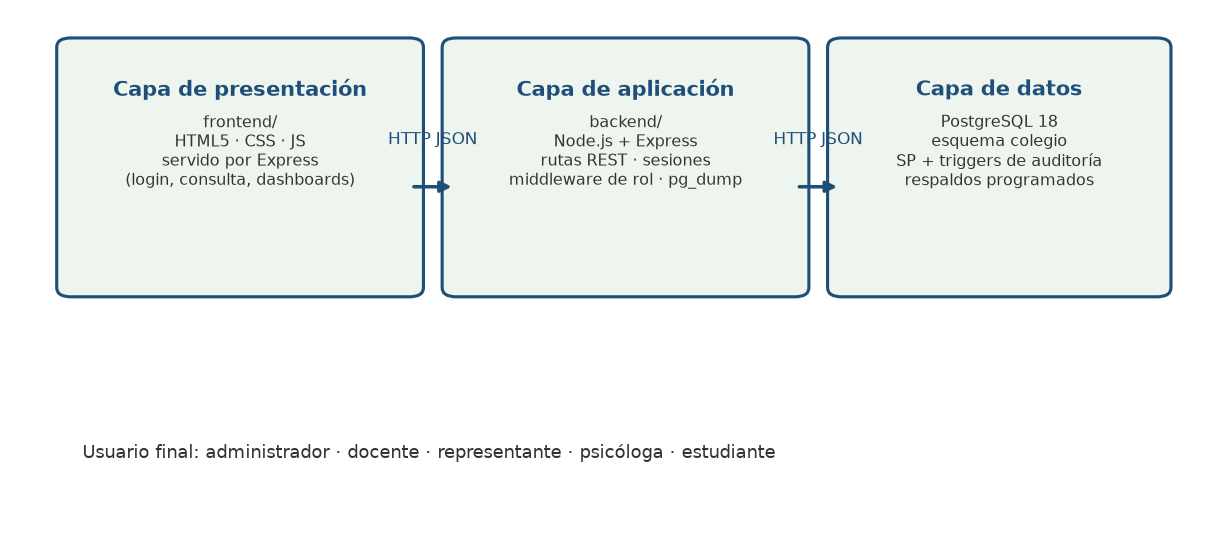
\includegraphics[width=0.92\textwidth]{evidencias/arquitectura.png}
\caption{Figura 1. El sistema se organiza en tres capas: frontend estático servido por Express, backend de API en Express y base de datos PostgreSQL; todas las operaciones críticas pasan por procedimientos almacenados y por el trigger de auditoría.}
\end{figure}


\subsection*{1.6 Usuarios y datos de prueba}
\addcontentsline{toc}{subsection}{1.6 Usuarios y datos de prueba}


\textbf{Tabla 2. Roles y usuarios del sistema.}


{\small
\begin{longtable}{|p{\dimexpr\textwidth/3-2\tabcolsep\relax}|p{\dimexpr\textwidth/3-2\tabcolsep\relax}|p{\dimexpr\textwidth/3-2\tabcolsep\relax}|}
\rowcolor{UTECblue}\color{white}\bfseries Rol & \color{white}\bfseries \# usuarios & \color{white}\bfseries Descripción \\ \hline
\endfirsthead
\rowcolor{UTECblue}\color{white}\bfseries Rol & \color{white}\bfseries \# usuarios & \color{white}\bfseries Descripción \\ \hline
\endhead
administrador & 1 & Gestión de catálogos, estudiantes, periodos, auditoría y respaldos \\ \hline
profesor & 5 & Registro de calificaciones de las materias asignadas \\ \hline
representante & 1 & Consulta de las notas de sus hijos \\ \hline
psicologo & 1 & Panel de rendimiento académico y alertas \\ \hline
estudiante & 1 & Consulta de sus propias notas (sin reportes ni datos ajenos) \\ \hline
\end{longtable}}


El conjunto de datos de prueba está compuesto por \textbf{110 estudiantes} (10 del seed inicial \texttt{06\_more\_data.sql} más 100 sintéticos generados por la migración \texttt{19\_datos\_sinteticos.sql}) a los que se suman los registros que los propios casos de prueba crean y limpian (la corrida de evidencias mostró hasta 139 estudiantes y 124 filas de nómina al momento de la captura). El \textbf{periodo activo} es el id 1 (''2026-2027 {$\cdot$} Primer Quimestre''), con ciclos ''Quimestre 1'' y parciales ''Parcial 1''. Se dispone además de 5 bloques materia+paralelo y de un representante con 15 hijos, datos utilizados por los casos automatizados.


\subsection*{1.7 Flujo general del sistema}
\addcontentsline{toc}{subsection}{1.7 Flujo general del sistema}


El recorrido principal, en el orden en que las operaciones se relacionan entre módulos, es el siguiente:


\begin{enumerate}[leftmargin=*]
\item El usuario inicia sesión (\texttt{login.html}); el sistema valida sus credenciales y muestra únicamente los módulos permitidos según su rol.
\item Desde el Dashboard, cada rol ve sus indicadores: el administrador (estudiantes, materias, notas, movimientos, respaldos), la profesora (sus materias y últimas notas), el representante (promedios de sus hijos) y la psicóloga (rendimiento y alertas).
\item El administrador gestiona Estudiantes (registro, búsqueda, paginación) y Matrículas por periodo y curso.
\item El administrador o la profesora gestionan Catálogos (cursos, ciclos, parciales, tipos) y asignaciones profesor-materia-periodo.
\item La profesora crea \textbf{actividades} (insumos: lecciones, tareas, talleres) en su materia y registra las notas por actividad; cada guardado recalcula automáticamente los promedios.
\item El representante y el estudiante consultan las notas (desglose por materia, promedio general y escala cualitativa), cada uno restringido a lo propio.
\item El administrador genera \textbf{Reportes} de promedios por periodo y curso, y revisa la \textbf{Auditoría} (quién cambió qué y cuándo).
\item La psicóloga revisa el \textbf{Rendimiento} académico con alertas de bajo desempeño para el acompañamiento.
\item El administrador genera y restaura \textbf{Respaldos} de la base de datos (\texttt{pg\_dump}) como mecanismo de recuperación.
\end{enumerate}


\section*{2. Metodología y plan de pruebas}
\addcontentsline{toc}{section}{2. Metodología y plan de pruebas}


\subsection*{2.1 Enfoque y fases}
\addcontentsline{toc}{subsection}{2.1 Enfoque y fases}


El proceso de V\&V se ejecutó en fases, alineadas con el \textbf{Plan de Mejoras v2} del repositorio (Fases 1--8). Cada fase combinó una tarea de verificación con una de validación:


{\small
\begin{longtable}{|p{\dimexpr\textwidth/4-2\tabcolsep\relax}|p{\dimexpr\textwidth/4-2\tabcolsep\relax}|p{\dimexpr\textwidth/4-2\tabcolsep\relax}|p{\dimexpr\textwidth/4-2\tabcolsep\relax}|}
\rowcolor{UTECblue}\color{white}\bfseries Fase & \color{white}\bfseries Actividad de verificación & \color{white}\bfseries Actividad de validación & \color{white}\bfseries Resultado \\ \hline
\endfirsthead
\rowcolor{UTECblue}\color{white}\bfseries Fase & \color{white}\bfseries Actividad de verificación & \color{white}\bfseries Actividad de validación & \color{white}\bfseries Resultado \\ \hline
\endhead
1 & Revisión del esquema de base de datos y migraciones (01--34) & Definición de las historias de usuario HU-01{\ldots}HU-09 & Corrección de migraciones (H1--H6) \\ \hline
2 & Revisión de rutas, middleware y procedimientos almacenados & Definición de criterios de aceptación por HU & Corrección de \texttt{search\_path} y SP (H5, H6, H10) \\ \hline
3 & Ejecución de pruebas de API (\texttt{e2e\_test.js}) & Comparación de resultados contra los criterios & 66/66 API PASS \\ \hline
4 & Ejecución de pruebas de UI (Playwright) & Observación del comportamiento del flujo real & 35/35 UI PASS \\ \hline
5 & Revisión de seeds y datos de prueba & Población y consulta de datos por rol & Remapeo de profesores y representante (H13, H14) \\ \hline
6 & Pruebas de aceptación (UAT) & Juicio del usuario final simulado & 7/7 UAT ACEPTADO \\ \hline
7 & Prueba Beta (7 días) & Uso real por 6 participantes & 0 errores funcionales \\ \hline
8 & Encuesta de satisfacción & Percepción de 89 usuarios & 4.8/5 (96\%) \\ \hline
\end{longtable}}


\subsection*{2.2 Estrategia de prueba por nivel}
\addcontentsline{toc}{subsection}{2.2 Estrategia de prueba por nivel}


\begin{enumerate}[leftmargin=*]
\item \textbf{Nivel estático:} inspección de código fuente, migraciones SQL y scripts de instalación. Fundamentalmente se revisaron:
\end{enumerate}


\begin{itemize}[leftmargin=*]
\item Las migraciones \texttt{0N\_*.sql} y la secuencia \texttt{01}--\texttt{34} (rollout ordenado).
\item Los procedimientos almacenados y triggers (auditoría, registro de calificaciones, ponderación de ciclos).
\item Los scripts \texttt{setup.ps1}, \texttt{seed-test-users.js} y \texttt{e2e\_test.js}.
\end{itemize}


\begin{enumerate}[leftmargin=*]
\item \textbf{Nivel de integración/API:} se ejecutó el script \texttt{backend/e2e\_test.js} (66 checks) que golpea las rutas REST con credenciales por rol y verifica en la base de datos el resultado de cada operación.
\item \textbf{Nivel de sistema/UI:} se ejecutó la suite Playwright (35 tests) sobre Chromium, con la base de datos compartida en ejecución serializada (workers = 1).
\item \textbf{Nivel de aceptación:} casos UAT (7), prueba Beta (7 días) y encuesta (89 usuarios).
\end{enumerate}


\subsection*{2.3 Entorno de pruebas}
\addcontentsline{toc}{subsection}{2.3 Entorno de pruebas}


{\small
\begin{longtable}{|p{\dimexpr\textwidth/2-2\tabcolsep\relax}|p{\dimexpr\textwidth/2-2\tabcolsep\relax}|}
\rowcolor{UTECblue}\color{white}\bfseries Elemento & \color{white}\bfseries Valor \\ \hline
\endfirsthead
\rowcolor{UTECblue}\color{white}\bfseries Elemento & \color{white}\bfseries Valor \\ \hline
\endhead
Sistema operativo & Windows / Linux (desarrollo) \\ \hline
Servidor local & API + frontend servidos por Express en \texttt{\url{http://localhost:3000}} \\ \hline
Base de datos & PostgreSQL 18, esquema \texttt{colegio} \\ \hline
Navegador de pruebas & Chromium (Chrome for Testing v153, del instalador de Playwright 1.63) \\ \hline
Navegadores de compatibilidad & Chrome y Edge (Beta) \\ \hline
Node.js & v24 \\ \hline
Editor / control de versiones & VSCode {$\cdot$} Git + GitHub \\ \hline
\end{longtable}}


\subsection*{2.4 Datos de prueba}
\addcontentsline{toc}{subsection}{2.4 Datos de prueba}


Los datos provienen de las migraciones del repositorio:


\begin{itemize}[leftmargin=*]
\item \textbf{10 estudiantes} del seed base \texttt{06\_more\_data.sql}, con sus profesores, asignaciones y notas iniciales.
\item \textbf{100 estudiantes sintéticos} añadidos por \texttt{19\_datos\_sinteticos.sql} (para ejercer paginación y reportes).
\item \textbf{Periodos:} 3 (activo = id 1 ''2026-2027 {$\cdot$} Primer Quimestre''), con ciclos y parciales.
\item \textbf{5 bloques} materia+paralelo usados por la consulta por bloques y por las asignaciones.
\item El \textbf{rol estudiante} (migración 21) permite a un alumno consultar únicamente sus propias notas.
\end{itemize}


Además, la suite automatizada \textbf{descubre los identificadores en tiempo de ejecución} (no los hardcodea) y \textbf{limpia los objetos E2E-\textbackslash\{\}}* que crea, de modo que la base permanece coherente entre corridas.


\subsection*{2.5 Criterios de entrada y salida}
\addcontentsline{toc}{subsection}{2.5 Criterios de entrada y salida}


\subsubsection*{Criterios de entrada}
\addcontentsline{toc}{subsubsection}{Criterios de entrada}


\begin{itemize}[leftmargin=*]
\item El repositorio está actualizado a \texttt{origin/main} con las migraciones 01--34 aplicadas.
\item La base de datos está reconstruible desde cero (\texttt{psql} + migraciones) y contiene el periodo activo.
\item El servidor se levanta con \texttt{npm start} y responde en el puerto 3000.
\item Como verificación de entorno, el login de los 4 roles principales completa con 200 OK.
\end{itemize}


\subsubsection*{Criterios de salida}
\addcontentsline{toc}{subsubsection}{Criterios de salida}


\begin{itemize}[leftmargin=*]
\item 100\% de los casos manuales (14/14), API (66/66), UI (35/35) y UAT (7/7) superados.
\item Cero hallazgos abiertos de severidad alta o media.
\item No se reportan errores funcionales en la prueba Beta.
\item Satisfacción global de la encuesta {$\geq$} 4.5/5.
\end{itemize}


\subsection*{2.6 Roles, responsables y cronograma}
\addcontentsline{toc}{subsection}{2.6 Roles, responsables y cronograma}


{\small
\begin{longtable}{|p{\dimexpr\textwidth/3-2\tabcolsep\relax}|p{\dimexpr\textwidth/3-2\tabcolsep\relax}|p{\dimexpr\textwidth/3-2\tabcolsep\relax}|}
\rowcolor{UTECblue}\color{white}\bfseries Rol en el proceso & \color{white}\bfseries Responsable & \color{white}\bfseries Actividades \\ \hline
\endfirsthead
\rowcolor{UTECblue}\color{white}\bfseries Rol en el proceso & \color{white}\bfseries Responsable & \color{white}\bfseries Actividades \\ \hline
\endhead
Analista de V\&V / tester de API & Vélez López Ricardo & Pruebas de API, entorno, evidencias, hallazgos H1--H15 \\ \hline
Tester de UI / documentación & Castro Espinoza Kevin Moisés & Suite Playwright, capturas, UAT, encuesta \\ \hline
Desarrollo / BD / despliegue & Panama Murillo Moises Antonio & Backend, base de datos, Docker, despliegue \\ \hline
Usuario final simulado (Beta) & Participantes B1--B6 & Prueba Beta y encuesta \\ \hline
\end{longtable}}


{\small
\begin{longtable}{|p{\dimexpr\textwidth/5-2\tabcolsep\relax}|p{\dimexpr\textwidth/5-2\tabcolsep\relax}|p{\dimexpr\textwidth/5-2\tabcolsep\relax}|p{\dimexpr\textwidth/5-2\tabcolsep\relax}|p{\dimexpr\textwidth/5-2\tabcolsep\relax}|}
\rowcolor{UTECblue}\color{white}\bfseries Actividad & \color{white}\bfseries Semana 1 & \color{white}\bfseries Semana 2 & \color{white}\bfseries Semana 3 & \color{white}\bfseries Semana 4 \\ \hline
\endfirsthead
\rowcolor{UTECblue}\color{white}\bfseries Actividad & \color{white}\bfseries Semana 1 & \color{white}\bfseries Semana 2 & \color{white}\bfseries Semana 3 & \color{white}\bfseries Semana 4 \\ \hline
\endhead
Revisión estática y corrección de hallazgos & X & X &  &  \\ \hline
Pruebas de API & X & X & X &  \\ \hline
Pruebas de UI (Playwright) &  & X & X &  \\ \hline
UAT &  &  & X & X \\ \hline
Prueba Beta (7 días) &  &  &  & X \\ \hline
Encuesta y análisis &  &  &  & X \\ \hline
Elaboración del informe final &  &  & X & X \\ \hline
\end{longtable}}


\subsection*{2.7 Riesgos y su mitigación}
\addcontentsline{toc}{subsection}{2.7 Riesgos y su mitigación}


{\small
\begin{longtable}{|p{\dimexpr\textwidth/3-2\tabcolsep\relax}|p{\dimexpr\textwidth/3-2\tabcolsep\relax}|p{\dimexpr\textwidth/3-2\tabcolsep\relax}|}
\rowcolor{UTECblue}\color{white}\bfseries Riesgo & \color{white}\bfseries Impacto & \color{white}\bfseries Mitigación aplicada \\ \hline
\endfirsthead
\rowcolor{UTECblue}\color{white}\bfseries Riesgo & \color{white}\bfseries Impacto & \color{white}\bfseries Mitigación aplicada \\ \hline
\endhead
Migraciones que fallan en instalación limpia & Bloqueo del entorno & Revisión estática H1--H6 y reconstrucción de base desde cero \\ \hline
Rutas que llaman a SP inexistentes o ambiguos & 500 en calificaciones & Corrección de llamadas H6 y H10 \\ \hline
Búsquedas con \texttt{search\_path} incorrecto & ''relación no existe'' & \texttt{ALTER DATABASE/ROLE ... SET search\_path TO colegio, public} (H5, H12, H15) \\ \hline
Seeds con profesores desalineados & Dashboard vacíos & Remapeo por email (H13, H14) \\ \hline
Suite frágil por IDs hardcodeados & Falsos negativos & Reescritura data-driven de \texttt{e2e\_test.js} (H7) \\ \hline
Playwright sin navegador en CI/local & Suite caída & Instalación de Chromium v1243 (H8) \\ \hline
\end{longtable}}


\subsection*{2.8 Herramientas de apoyo}
\addcontentsline{toc}{subsection}{2.8 Herramientas de apoyo}


{\small
\begin{longtable}{|p{\dimexpr\textwidth/2-2\tabcolsep\relax}|p{\dimexpr\textwidth/2-2\tabcolsep\relax}|}
\rowcolor{UTECblue}\color{white}\bfseries Herramienta & \color{white}\bfseries Uso \\ \hline
\endfirsthead
\rowcolor{UTECblue}\color{white}\bfseries Herramienta & \color{white}\bfseries Uso \\ \hline
\endhead
\texttt{@playwright/test} 1.63 & Orquestación de pruebas E2E, reporter de lista y HTML \\ \hline
Node.js (fetch/axios) & Pruebas de API en \texttt{e2e\_test.js} \\ \hline
Chromium headless & Ejecución de capturas y de la suite UI \\ \hline
Git / GitHub & Control de versiones, revisión de cambios entre commits (origen de H1--H15) \\ \hline
python-docx + Chromium print & Generación de los artefactos finales (PDF y DOCX) del informe \\ \hline
matplotlib & Gráficos de resultados de la encuesta y métricas \\ \hline
Google Forms (simulado) & Instrumento de la encuesta de satisfacción \\ \hline
\end{longtable}}


\section*{3. Técnica Personas}
\addcontentsline{toc}{section}{3. Técnica Personas}


\subsection*{3.1 Justificación de la técnica}
\addcontentsline{toc}{subsection}{3.1 Justificación de la técnica}


La técnica \textbf{Personas} consiste en crear arquetipos de usuarios finales basados en datos realistas (edad, rol, escolaridad, experiencia tecnológica, objetivos y frustraciones) para guiar el diseño de producto y, en este caso, \textbf{orientar el diseño de las pruebas}. Se definieron cuatro personas que representan los perfiles que interactúan con el sistema, cada una con un \textbf{foco de pruebas} distinto: el control administrativo, la carga de notas, la consulta remota y el análisis de rendimiento.


\subsection*{3.2 Persona 1 --- ''Lic. Moisés Panamá'' (Administrador / Coordinador Académico)}
\addcontentsline{toc}{subsection}{3.2 Persona 1 --- ''Lic. Moisés Panamá'' (Administrador / Coordinador Académico)}

\begin{figure}[H]
  \centering
  
\includegraphics[width=0.38\textwidth]{evidencias/persona_moises.png}
  \caption{Arquetipo ``Lic. Moisés Panamá'' --- Administrador / Coordinador Académico}
  \label{fig:persona-moises}
\end{figure}

{\small
\begin{longtable}{|p{\dimexpr\textwidth/2-2\tabcolsep\relax}|p{\dimexpr\textwidth/2-2\tabcolsep\relax}|}
\rowcolor{UTECblue}\color{white}\bfseries Atributo & \color{white}\bfseries Detalle \\ \hline
\endfirsthead
\rowcolor{UTECblue}\color{white}\bfseries Atributo & \color{white}\bfseries Detalle \\ \hline
\endhead
Edad & 35 años \\ \hline
Rol & Coordinador Académico de la Unidad Educativa \\ \hline
Escolaridad & Licenciado en Ciencias de la Educación \\ \hline
Experiencia tecnológica & Media: ofimática, correo y sistemas web institucionales \\ \hline
Entorno & Computadora de escritorio en la administración \\ \hline
\end{longtable}}


\textbf{Objetivos:}


\begin{itemize}[leftmargin=*]
\item Tener un control centralizado y trazable de estudiantes, materias, periodos académicos y calificaciones.
\item Garantizar la integridad de la información: que nadie altere una nota sin dejar registro.
\item Generar reportes oficiales de promedios por periodo para la dirección.
\end{itemize}


\textbf{Necesidades:}


\begin{itemize}[leftmargin=*]
\item Crear y mantener el catálogo de estudiantes, materias y periodos.
\item Asignar y activar \textbf{un único periodo académico} en uso.
\item Auditar cualquier cambio de los docentes y propios.
\item Respaldar la base de datos para evitar pérdida de información.
\end{itemize}


\textbf{Frustraciones:}


\begin{itemize}[leftmargin=*]
\item Teme que un docente modifique notas en papel sin dejar rastro.
\item Le incomodan los Excel compartidos porque pierden la trazabilidad.
\item El cambio de periodo debe ser sencillo y seguro (solo un activo a la vez).
\end{itemize}


\textbf{Relación con el sistema:} utiliza la gestión de estudiantes, materias, periodos, auditoría y respaldos. Orienta la prioridad de las historias de administración, control de acceso y auditoría (HU-01, HU-02, HU-06, HU-07, HU-08) y de los casos CP-01{\ldots}CP-04, CP-10{\ldots}CP-12.


\subsection*{3.3 Persona 2 --- ''Prof. Elena Romero'' (Docente)}
\addcontentsline{toc}{subsection}{3.3 Persona 2 --- ''Prof. Elena Romero'' (Docente)}

\begin{figure}[H]
  \centering
  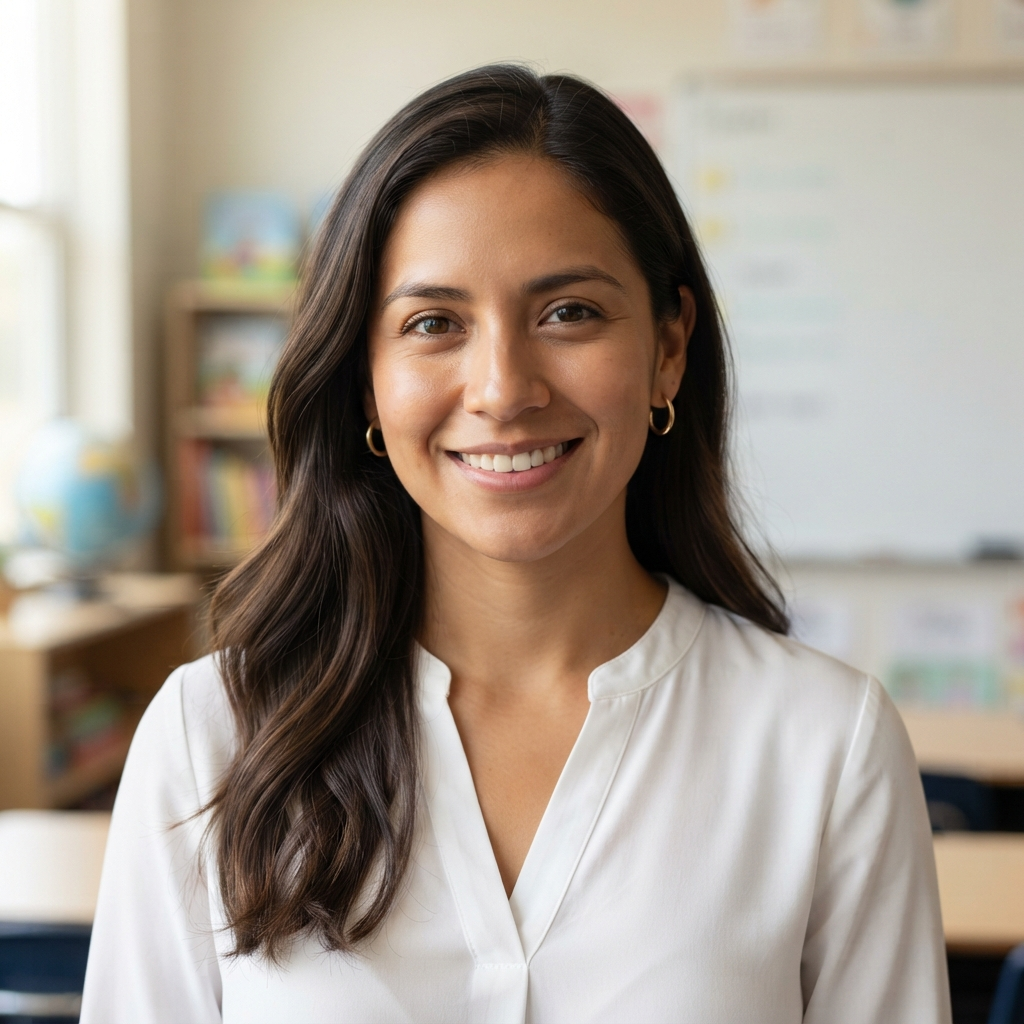
\includegraphics[width=0.38\textwidth]{evidencias/persona_elena.png}
  \caption{Arquetipo ``Prof. Elena Romero'' --- Docente de Ciencias Naturales}
  \label{fig:persona-elena}
\end{figure}

{\small
\begin{longtable}{|p{\dimexpr\textwidth/2-2\tabcolsep\relax}|p{\dimexpr\textwidth/2-2\tabcolsep\relax}|}
\rowcolor{UTECblue}\color{white}\bfseries Atributo & \color{white}\bfseries Detalle \\ \hline
\endfirsthead
\rowcolor{UTECblue}\color{white}\bfseries Atributo & \color{white}\bfseries Detalle \\ \hline
\endhead
Edad & 29 años \\ \hline
Rol & Profesora de Ciencias Naturales (Octavo EGB) \\ \hline
Escolaridad & Ing. en Ciencias Naturales \\ \hline
Experiencia tecnológica & Media-alta: Moodle, Google Classroom \\ \hline
Entorno & Laptop personal, internet del plantel \\ \hline
\end{longtable}}


\textbf{Objetivos:}


\begin{itemize}[leftmargin=*]
\item Registrar las calificaciones de sus estudiantes de forma rápida y sin errores de cálculo.
\item Ver únicamente las notas de las materias que le corresponden.
\item Confiar en que el promedio se calcula con la fórmula oficial (80\% parciales + 20\% examen).
\end{itemize}


\textbf{Necesidades:}


\begin{itemize}[leftmargin=*]
\item Entrar al módulo ''Registrar Nota'' y ver su materia asignada.
\item Digitar notas parciales y guardarlas en masa (tabla completa).
\item Corregir una nota (upsert) con la seguridad de que el cambio queda auditado.
\item Consultar las notas ya registradas del periodo.
\end{itemize}


\textbf{Frustraciones:}


\begin{itemize}[leftmargin=*]
\item En libros físicos pierde tiempo sumando promedios a mano.
\item Le preocupa equivocarse de estudiante al llenar la planilla.
\end{itemize}


\textbf{Relación con el sistema:} protagonista de las historias de registro de calificaciones (HU-03) y de las validaciones de rango 0--10 y asignación de materia (un profesor solo califica sus materias). Ejercida en los casos CP-05{\ldots}CP-07 y los tests automatizados de \texttt{calificaciones.spec.cjs}.


\subsection*{3.4 Persona 3 --- ''Sr. Fernando Castillo'' (Representante / Padre de familia)}
\addcontentsline{toc}{subsection}{3.4 Persona 3 --- ''Sr. Fernando Castillo'' (Representante / Padre de familia)}

\begin{figure}[H]
  \centering
  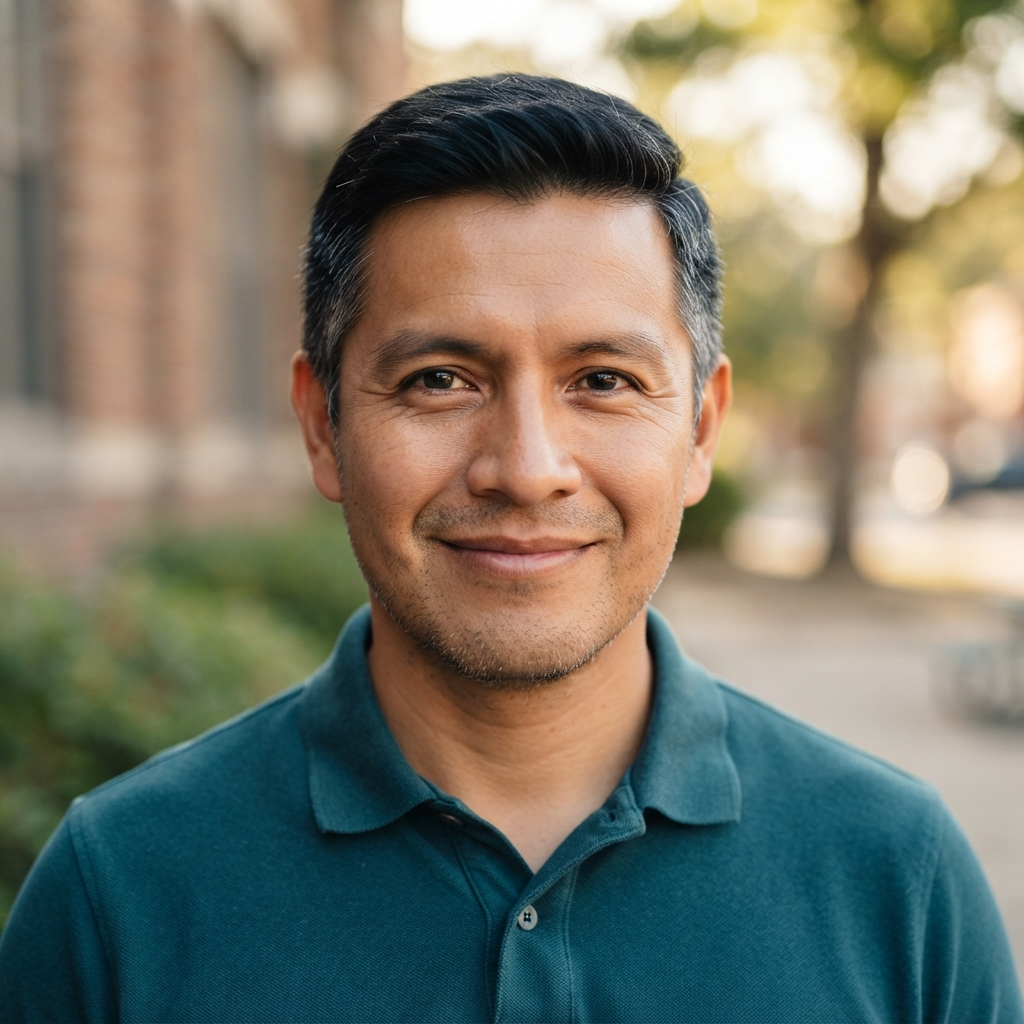
\includegraphics[width=0.38\textwidth]{evidencias/persona_fernando.png}
  \caption{Arquetipo ``Sr. Fernando Castillo'' --- Representante / Padre de familia}
  \label{fig:persona-fernando}
\end{figure}

{\small
\begin{longtable}{|p{\dimexpr\textwidth/2-2\tabcolsep\relax}|p{\dimexpr\textwidth/2-2\tabcolsep\relax}|}
\rowcolor{UTECblue}\color{white}\bfseries Atributo & \color{white}\bfseries Detalle \\ \hline
\endfirsthead
\rowcolor{UTECblue}\color{white}\bfseries Atributo & \color{white}\bfseries Detalle \\ \hline
\endhead
Edad & 41 años \\ \hline
Rol & Representante legal de un estudiante de Octavo EGB \\ \hline
Escolaridad & Bachiller \\ \hline
Experiencia tecnológica & Baja-media: redes sociales, WhatsApp, portales web \\ \hline
Entorno & Móvil o computador familiar \\ \hline
\end{longtable}}


\textbf{Objetivos:}


\begin{itemize}[leftmargin=*]
\item Consultar las notas de sus hijos sin acudir al plantel.
\item Ver los promedios por materia y el promedio general de cada periodo.
\item Identificar a tiempo si su representado está en riesgo académico.
\end{itemize}


\textbf{Necesidades:}


\begin{itemize}[leftmargin=*]
\item Ingresar con un usuario propio (sin permisos de administración).
\item Ver \textbf{solo} la información de sus hijos.
\item Navegación simple: seleccionar el hijo y ver el cuadro de notas y promedios.
\end{itemize}


\textbf{Frustraciones:}


\begin{itemize}[leftmargin=*]
\item Los formatos impresos se pierden en la mochila.
\item No entiende los promedios sin una escala clara.
\end{itemize}


\textbf{Relación con el sistema:} valida la historia de consulta de notas (HU-04) y el control de visibilidad por rol; fue usuario clave de la prueba Beta (B1).


\subsection*{3.5 Persona 4 --- ''Lic. María Torres'' (Psicóloga Educativa / DECE)}
\addcontentsline{toc}{subsection}{3.5 Persona 4 --- ''Lic. María Torres'' (Psicóloga Educativa / DECE)}

\begin{figure}[H]
  \centering
  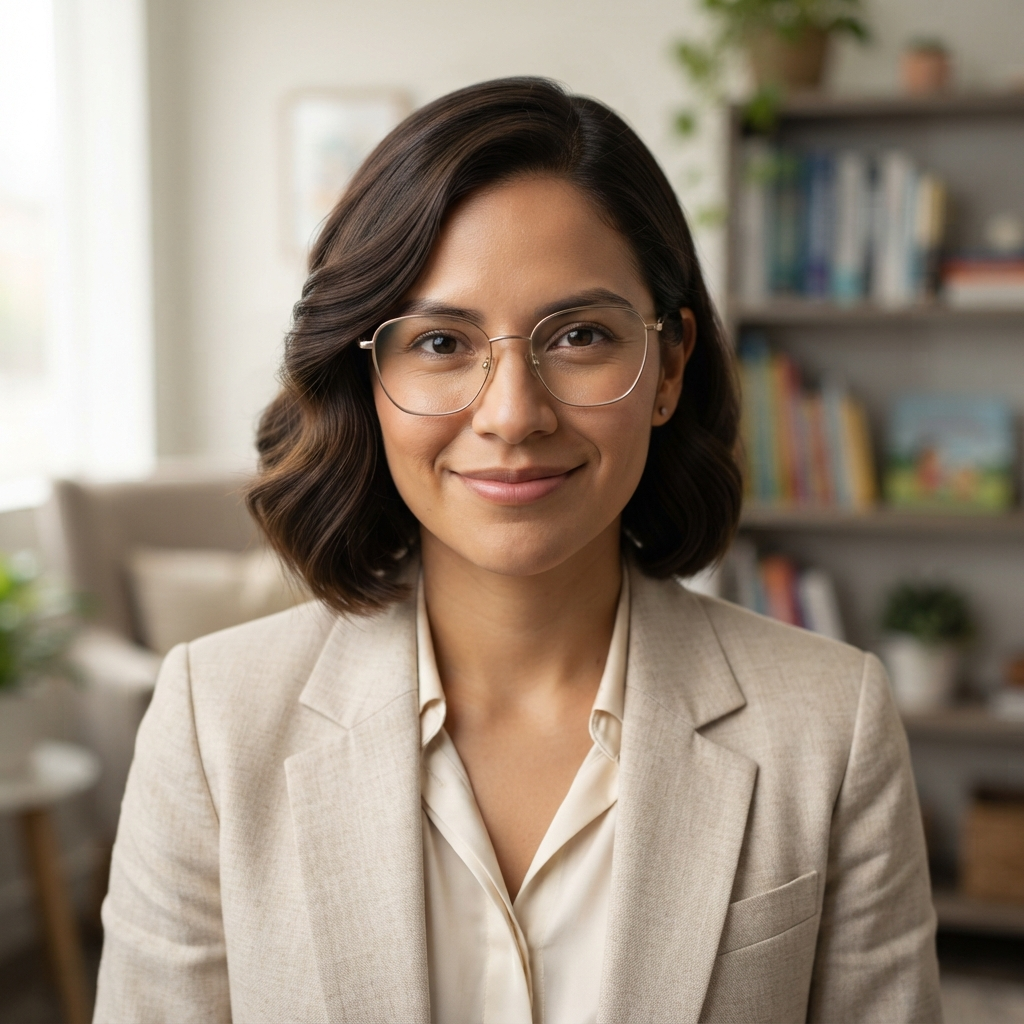
\includegraphics[width=0.38\textwidth]{evidencias/persona_maria.png}
  \caption{Arquetipo ``Lic. María Torres'' --- Psicóloga Educativa / DECE}
  \label{fig:persona-maria}
\end{figure}

{\small
\begin{longtable}{|p{\dimexpr\textwidth/2-2\tabcolsep\relax}|p{\dimexpr\textwidth/2-2\tabcolsep\relax}|}
\rowcolor{UTECblue}\color{white}\bfseries Atributo & \color{white}\bfseries Detalle \\ \hline
\endfirsthead
\rowcolor{UTECblue}\color{white}\bfseries Atributo & \color{white}\bfseries Detalle \\ \hline
\endhead
Edad & 33 años \\ \hline
Rol & Psicóloga del Departamento de Consejería Estudiantil \\ \hline
Escolaridad & Licenciada en Psicología Educativa \\ \hline
Experiencia tecnológica & Media: sistemas de reportes institucionales \\ \hline
Entorno & Computadora del DECE \\ \hline
\end{longtable}}


\textbf{Objetivos:}


\begin{itemize}[leftmargin=*]
\item Identificar estudiantes con bajo rendimiento o riesgo académico para intervención temprana.
\item Ver el desempeño por quimestre y por materia de forma agregada.
\item Preparar listados de estudiantes que requieren acompañamiento.
\end{itemize}


\textbf{Necesidades:}


\begin{itemize}[leftmargin=*]
\item Pantalla de ''Rendimiento'' con resumen de alertas.
\item Detalle por estudiante con promedios por materia y por periodo.
\item Solo lectura de indicadores (no modifica notas).
\end{itemize}


\textbf{Frustraciones:}


\begin{itemize}[leftmargin=*]
\item Antes dependía de capturas que le pasara el docente.
\item Necesita datos objetivos, no impresiones.
\end{itemize}


\textbf{Relación con el sistema:} valida el módulo de rendimiento académico (HU-09) tanto en las pruebas automatizadas como en las UAT (CP-13, \texttt{psicologo.spec.cjs}, UAT-07).


\subsection*{3.6 Cómo orientaron las personas el diseño de las pruebas}
\addcontentsline{toc}{subsection}{3.6 Cómo orientaron las personas el diseño de las pruebas}


{\small
\begin{longtable}{|p{\dimexpr\textwidth/2-2\tabcolsep\relax}|p{\dimexpr\textwidth/2-2\tabcolsep\relax}|}
\rowcolor{UTECblue}\color{white}\bfseries Persona & \color{white}\bfseries Foco de pruebas resultante \\ \hline
\endfirsthead
\rowcolor{UTECblue}\color{white}\bfseries Persona & \color{white}\bfseries Foco de pruebas resultante \\ \hline
\endhead
Moisés (admin) & Gestión de estudiantes/materias/periodos, activación de un solo periodo, panel de auditoría y respaldos {$\rightarrow$} HU-01, HU-02, HU-06, HU-07, HU-08 \\ \hline
Elena (profesor) & Validaciones de rango (0--10), autorización por materia, guardado masivo {$\rightarrow$} HU-03 \\ \hline
Fernando (representante) & Consulta con restricción por rol, legibilidad de promedios y escala cualitativa {$\rightarrow$} HU-04, HU-05 \\ \hline
María (psicóloga) & Panel de rendimiento, alertas y detalle por estudiante {$\rightarrow$} HU-09 \\ \hline
\end{longtable}}


Estas personas permitieron derivar historias de usuario reales y definir \textbf{criterios de aceptación orientados a la frecuencia y al valor de uso de cada perfil}, como los que se detallan en el capítulo siguiente.


\hrule\vspace{0.4em}


\section*{4. Historias de usuario y criterios de aceptación}
\addcontentsline{toc}{section}{4. Historias de usuario y criterios de aceptación}


\subsection*{4.1 Formato}
\addcontentsline{toc}{subsection}{4.1 Formato}


Las historias usan el formato estándar \textbf{''Como [rol], quiero [funcionalidad], para [beneficio]''}, acompañadas de criterios de aceptación verificables. Cada historia tiene un código \textbf{HU-XX} y una prioridad \textbf{MoSCoW} (\textbf{Must have}: flujo académico indispensable; \textbf{Should have}: importante pero no bloqueante) que se usa como referencia en los casos de prueba manuales (CP), automatizados (AUT) y de aceptación (UAT).


\subsection*{4.2 HU-01 --- Iniciar sesión (administrador) \textbf{(Must have)}}
\addcontentsline{toc}{subsection}{4.2 HU-01 --- Iniciar sesión (administrador) \textbf{(Must have)}}


\textbf{Como} administrador, \textbf{quiero} iniciar sesión con mi correo y contraseña, \textbf{para} acceder a la gestión del sistema.


\textbf{Criterios de aceptación:}


\begin{enumerate}[leftmargin=*]
\item CA-1: Con credenciales válidas, el usuario es redirigido al dashboard.
\item CA-2: Con contraseña incorrecta, se muestra un mensaje de error y no se inicia sesión.
\item CA-3: Solo los usuarios con \texttt{activo = true} pueden ingresar.
\end{enumerate}


\textbf{Evidencia de cumplimiento:} CP-01, CP-02, CP-14; AUT-01, AUT-02, AUT-09; UAT-01; 5 logins por rol en la suite API.


\subsection*{4.3 HU-02 --- Gestión de estudiantes \textbf{(Must have)}}
\addcontentsline{toc}{subsection}{4.3 HU-02 --- Gestión de estudiantes \textbf{(Must have)}}


\textbf{Como} administrador, \textbf{quiero} registrar, listar y buscar estudiantes, \textbf{para} mantener el registro de matrícula actualizado.


\textbf{Criterios de aceptación:}


\begin{enumerate}[leftmargin=*]
\item CA-1: Se crea un estudiante con cédula única, nombres, apellidos, fecha de nacimiento y representante.
\item CA-2: La búsqueda por cédula o nombre devuelve las coincidencias.
\item CA-3: Una cédula duplicada es rechazada con mensaje claro (HTTP 409).
\end{enumerate}


\textbf{Evidencia de cumplimiento:} CP-03, CP-04; AUT-03, AUT-04; UAT-02; checks de paginación de la suite API (139 estudiantes).


\subsection*{4.4 HU-03 --- Registro de calificaciones (profesor) \textbf{(Must have)}}
\addcontentsline{toc}{subsection}{4.4 HU-03 --- Registro de calificaciones (profesor) \textbf{(Must have)}}


\textbf{Como} profesor, \textbf{quiero} registrar las notas de mis estudiantes en las materias que tengo asignadas, \textbf{para} que el promedio se calcule automáticamente.


\textbf{Criterios de aceptación:}


\begin{enumerate}[leftmargin=*]
\item CA-1: El profesor solo ve y edita calificaciones de materias asignadas en el periodo activo.
\item CA-2: Las notas deben estar en el rango 0--10; valores fuera de rango se rechazan.
\item CA-3: El guardado masivo registra todas las celdas modificadas en una sola transacción.
\item CA-4: Si cambia una nota existente, se sobrescribe (upsert) y el cambio queda auditado.
\item CA-5: El profesor no puede registrar notas de una materia que no tiene asignada (HTTP 403).
\end{enumerate}


\textbf{Evidencia de cumplimiento:} CP-05, CP-06, CP-07; AUT-05; checks de calificaciones de la suite API (lote con parcial/ciclo, parcial inválido {$\rightarrow$} 400).


\subsection*{4.5 HU-04 --- Consulta de calificaciones por estudiante \textbf{(Must have)}}
\addcontentsline{toc}{subsection}{4.5 HU-04 --- Consulta de calificaciones por estudiante \textbf{(Must have)}}


\textbf{Como} representante, \textbf{quiero} consultar las notas y promedios de mis hijos, \textbf{para} dar seguimiento a su rendimiento académico.


\textbf{Criterios de aceptación:}


\begin{enumerate}[leftmargin=*]
\item CA-1: El representante ve únicamente las notas de sus hijos.
\item CA-2: Se muestran las notas por materia, el promedio por materia y el promedio general del periodo.
\item CA-3: Se muestra la escala cualitativa oficial (Domina / Alcanza / Próximo / No alcanza) según el promedio.
\end{enumerate}


\textbf{Evidencia de cumplimiento:} CP-08; AUT-06; UAT-04; checks del dashboard de representante (15 hijos con promedios) y del desglose por materia.


\subsection*{4.6 HU-05 --- Reportes de promedios por periodo \textbf{(Should have)}}
\addcontentsline{toc}{subsection}{4.6 HU-05 --- Reportes de promedios por periodo \textbf{(Should have)}}


\textbf{Como} representante y administrador, \textbf{quiero} ver el reporte de promedios del periodo, \textbf{para} conocer el desempeño general del curso.


\textbf{Criterios de aceptación:}


\begin{enumerate}[leftmargin=*]
\item CA-1: El reporte lista estudiantes ordenados por promedio descendente.
\item CA-2: Se puede filtrar por curso y por materia.
\item CA-3: El promedio mostrado coincide con la fórmula oficial del sistema.
\end{enumerate}


\textbf{Evidencia de cumplimiento:} CP-09; UAT-05; checks de paginación de la suite API (reportes con 124 filas y filtro sin-curso).


\subsection*{4.7 HU-06 --- Auditar cambios (administrador) \textbf{(Should have)}}
\addcontentsline{toc}{subsection}{4.7 HU-06 --- Auditar cambios (administrador) \textbf{(Should have)}}


\textbf{Como} administrador, \textbf{quiero} consultar el historial de cambios, \textbf{para} garantizar la integridad y trazabilidad de la información.


\textbf{Criterios de aceptación:}


\begin{enumerate}[leftmargin=*]
\item CA-1: Solo el rol administrador puede acceder al panel de auditoría.
\item CA-2: Se registran INSERT, UPDATE y DELETE con datos antes/después en JSONB.
\item CA-3: Cada registro indica el usuario de la aplicación que realizó el cambio.
\item CA-4: La tabla \texttt{auditoria} es de solo lectura + inserción (nadie modifica el historial).
\end{enumerate}


\textbf{Evidencia de cumplimiento:} CP-10, CP-11; AUT-03, AUT-07; UAT-06; checks de auditoría de la suite API (total 855 registros en la corrida, usuario de la app, resumen por categorías, filtros y 403 para Elena).


\subsection*{4.8 HU-07 --- Activación de un único periodo académico \textbf{(Should have)}}
\addcontentsline{toc}{subsection}{4.8 HU-07 --- Activación de un único periodo académico \textbf{(Should have)}}


\textbf{Como} administrador, \textbf{quiero} activar un periodo académico y que exista solo uno activo, \textbf{para} que todas las operaciones operen sobre el periodo correcto.


\textbf{Criterios de aceptación:}


\begin{enumerate}[leftmargin=*]
\item CA-1: Solo puede existir un periodo con \texttt{activo = TRUE} (reforzado por índice parcial y trigger).
\item CA-2: Al activar un nuevo periodo, los anteriores quedan inactivos automáticamente.
\end{enumerate}


\textbf{Evidencia de cumplimiento:} CP-12; revisión estática del índice parcial y del trigger; chequeo del periodo activo id=1 en la suite API.


\subsection*{4.9 HU-08 --- Respaldo de la base de datos \textbf{(Should have)}}
\addcontentsline{toc}{subsection}{4.9 HU-08 --- Respaldo de la base de datos \textbf{(Should have)}}


\textbf{Como} administrador, \textbf{quiero} crear y programar respaldos de la base de datos, \textbf{para} prevenir la pérdida de información.


\textbf{Criterios de aceptación:}


\begin{enumerate}[leftmargin=*]
\item CA-1: Se puede generar un respaldo manual (\texttt{pg\_dump}) desde el panel.
\item CA-2: Se puede programar un respaldo diario con \texttt{node-cron}.
\item CA-3: Los respaldos pueden listarse, descargarse y eliminarse (solo admin).
\end{enumerate}


\textbf{Evidencia de cumplimiento:} CP-11 (restricción), AUT-07; checks de respaldos de la suite API (respaldo manual nombrado y historial paginado de 5 filas).


\subsection*{4.10 HU-09 --- Rendimiento académico (psicóloga) \textbf{(Should have)}}
\addcontentsline{toc}{subsection}{4.10 HU-09 --- Rendimiento académico (psicóloga) \textbf{(Should have)}}


\textbf{Como} psicóloga, \textbf{quiero} ver el rendimiento académico y las alertas de bajo desempeño, \textbf{para} identificar a los estudiantes que requieren acompañamiento.


\textbf{Criterios de aceptación:}


\begin{enumerate}[leftmargin=*]
\item CA-1: El panel muestra resumen (total, bajo rendimiento, destacados, promedio general).
\item CA-2: Se listan estudiantes con promedios por quimestre y estado (En Inicio / En Proceso / Logro Esperado / Logro Destacado).
\item CA-3: Un clic en el estudiante abre el detalle con notas por materia y por periodo.
\end{enumerate}


\textbf{Evidencia de cumplimiento:} CP-13; AUT-08; UAT-07; checks de la suite API (paginado + resumen con 111 estudiantes y 10 alertas).


\subsection*{4.11 Matriz de trazabilidad}
\addcontentsline{toc}{subsection}{4.11 Matriz de trazabilidad}


\textbf{Tabla 4. Matriz de trazabilidad (Historias {$\rightarrow$} Pruebas).}


{\small
\begin{longtable}{|p{\dimexpr\textwidth/4-2\tabcolsep\relax}|p{\dimexpr\textwidth/4-2\tabcolsep\relax}|p{\dimexpr\textwidth/4-2\tabcolsep\relax}|p{\dimexpr\textwidth/4-2\tabcolsep\relax}|}
\rowcolor{UTECblue}\color{white}\bfseries Historia & \color{white}\bfseries Casos manuales & \color{white}\bfseries Casos automatizados UI & \color{white}\bfseries Casos UAT \\ \hline
\endfirsthead
\rowcolor{UTECblue}\color{white}\bfseries Historia & \color{white}\bfseries Casos manuales & \color{white}\bfseries Casos automatizados UI & \color{white}\bfseries Casos UAT \\ \hline
\endhead
HU-01 Login & CP-01, CP-02, CP-14 & AUT-01, AUT-02, AUT-09 & UAT-01 \\ \hline
HU-02 Estudiantes & CP-03, CP-04 & AUT-03, AUT-04 & UAT-02 \\ \hline
HU-03 Calificaciones & CP-05, CP-06, CP-07 & AUT-05 & UAT-03 \\ \hline
HU-04 Consulta & CP-08 & AUT-06 & UAT-04 \\ \hline
HU-05 Reportes & CP-09 & --- & UAT-05 \\ \hline
HU-06 Auditoría & CP-10, CP-11 & AUT-03, AUT-07 & UAT-06 \\ \hline
HU-07 Periodo activo & CP-12 & --- & --- \\ \hline
HU-08 Respaldos & CP-11 & AUT-07 & --- \\ \hline
HU-09 Psicóloga & CP-13 & AUT-08 & UAT-07 \\ \hline
\end{longtable}}


\section*{5. Casos de prueba manuales}
\addcontentsline{toc}{section}{5. Casos de prueba manuales}


\subsection*{5.1 Objetivo y método}
\addcontentsline{toc}{subsection}{5.1 Objetivo y método}


Se diseñaron \textbf{14 casos de prueba manuales (CP-01 {\ldots} CP-14)} que cubren transversalmente las 9 historias de usuario. Se ejecutaron dos técnicas:


\begin{enumerate}[leftmargin=*]
\item \textbf{Pruebas funcionales sobre la interfaz web} (login, dashboards, búsquedas, consultas, auditoría, psicóloga, logout), documentadas con capturas de pantalla.
\item \textbf{Pruebas de validación de negocio sobre la API} (409 de cédula duplicada, 400 de nota fuera de rango, 400 de fechas de periodo, 403 de materia no asignada, reportes y auditoría), documentadas en \texttt{evidencias/pruebas\_api\_manuales.txt}.
\end{enumerate}


\textbf{Estado global: 14/14 casos ejecutados {$\cdot$} 14 PASS {$\cdot$} 0 FAIL.}


\subsection*{5.2 CP-01 --- Login exitoso (administrador)}
\addcontentsline{toc}{subsection}{5.2 CP-01 --- Login exitoso (administrador)}


{\small
\begin{longtable}{|p{\dimexpr\textwidth/2-2\tabcolsep\relax}|p{\dimexpr\textwidth/2-2\tabcolsep\relax}|}
\rowcolor{UTECblue}\color{white}\bfseries Campo & \color{white}\bfseries Detalle \\ \hline
\endfirsthead
\rowcolor{UTECblue}\color{white}\bfseries Campo & \color{white}\bfseries Detalle \\ \hline
\endhead
Historia / Criterio & HU-01 / CA-1 \\ \hline
Precondiciones & Usuario \texttt{admin@uteq.edu.ec} activo; servidor en \texttt{localhost:3000} \\ \hline
Datos de prueba & \texttt{admin@uteq.edu.ec} / \texttt{UTEQ2026} \\ \hline
Pasos & 1) Abrir \texttt{login.html}. 2) Ingresar correo y contraseña. 3) Enviar el formulario. \\ \hline
Resultado esperado & Redirección a \texttt{dashboard.html}, saludo ''Bienvenido'' y rol \texttt{administrador} \\ \hline
Resultado obtenido & Redirección correcta; \texttt{\#bienvenida} = ''Bienvenido''; \texttt{\#rol} = administrador \\ \hline
Estado & {\color{green!60!black}{$\checkmark$}} PASS \\ \hline
\end{longtable}}


\begin{figure}[H]
\centering
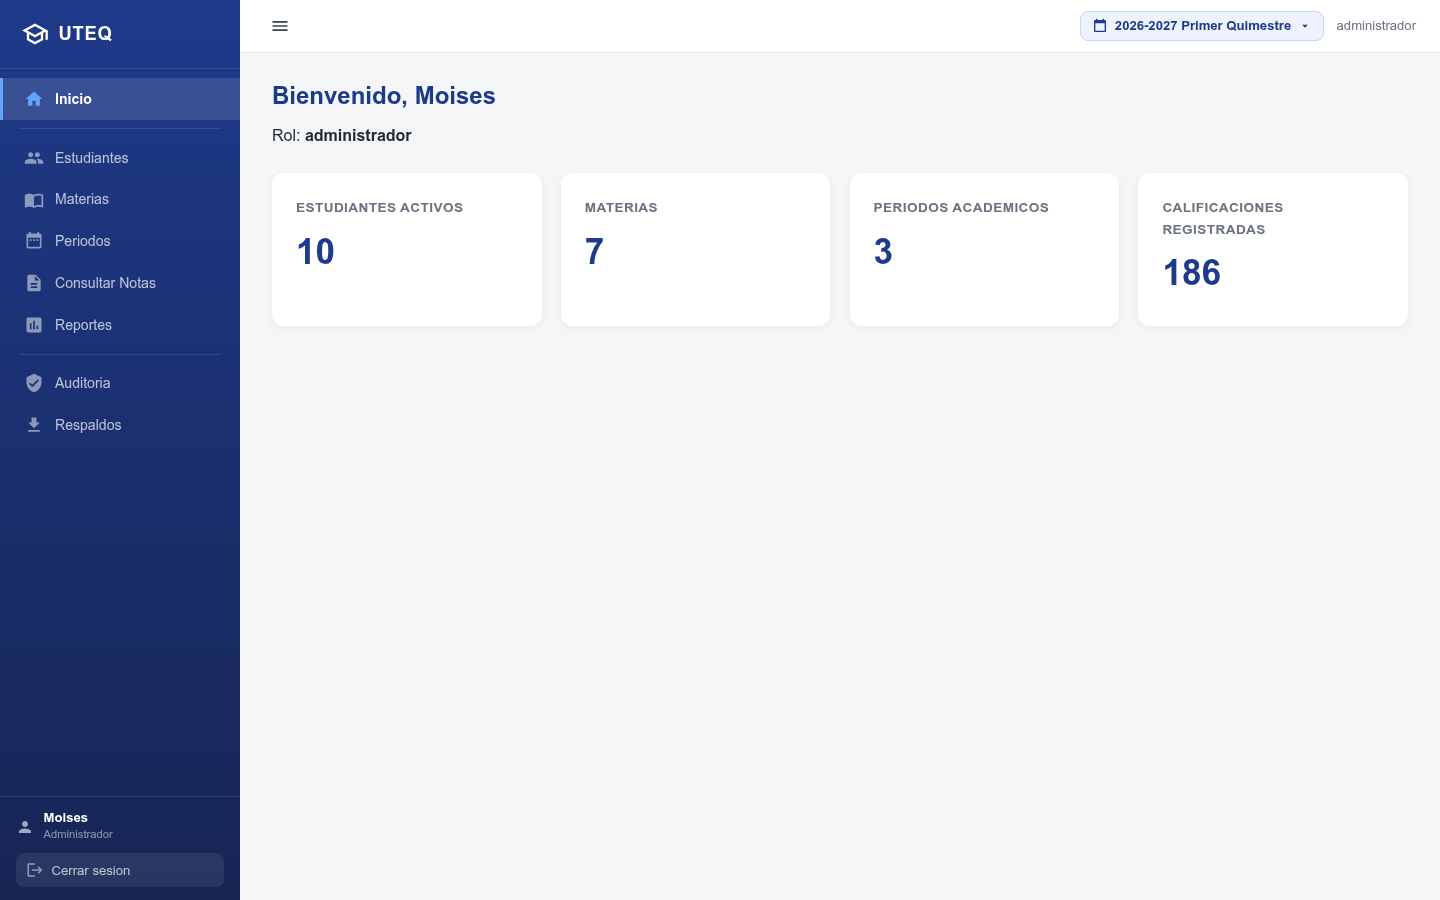
\includegraphics[width=0.92\textwidth]{evidencias/playwright-01-login-admin.png}
\caption{Figura 6. Captura del flujo de login exitoso del administrador (evidencia \texttt{playwright-01-login-admin.png}).}
\end{figure}


\textbf{Verificación adicional:} el mismo flujo se repitió con éxito para los roles profesor, representante y psicóloga (tests AUT-01 del capítulo 6).


\subsection*{5.3 CP-02 --- Login con contraseña incorrecta}
\addcontentsline{toc}{subsection}{5.3 CP-02 --- Login con contraseña incorrecta}


{\small
\begin{longtable}{|p{\dimexpr\textwidth/2-2\tabcolsep\relax}|p{\dimexpr\textwidth/2-2\tabcolsep\relax}|}
\rowcolor{UTECblue}\color{white}\bfseries Campo & \color{white}\bfseries Detalle \\ \hline
\endfirsthead
\rowcolor{UTECblue}\color{white}\bfseries Campo & \color{white}\bfseries Detalle \\ \hline
\endhead
Historia / Criterio & HU-01 / CA-2 \\ \hline
Precondiciones & --- \\ \hline
Datos de prueba & \texttt{admin@uteq.edu.ec} / \texttt{clave\_equivocada} \\ \hline
Pasos & 1) Abrir \texttt{login.html}. 2) Ingresar correo válido y contraseña inválida. 3) Enviar. \\ \hline
Resultado esperado & Mensaje de error visible, sin sesión creada, permanece en login \\ \hline
Resultado obtenido & \texttt{\#error} visible con mensaje de credenciales inválidas; sin redirección \\ \hline
Estado & {\color{green!60!black}{$\checkmark$}} PASS \\ \hline
\end{longtable}}


\begin{figure}[H]
\centering
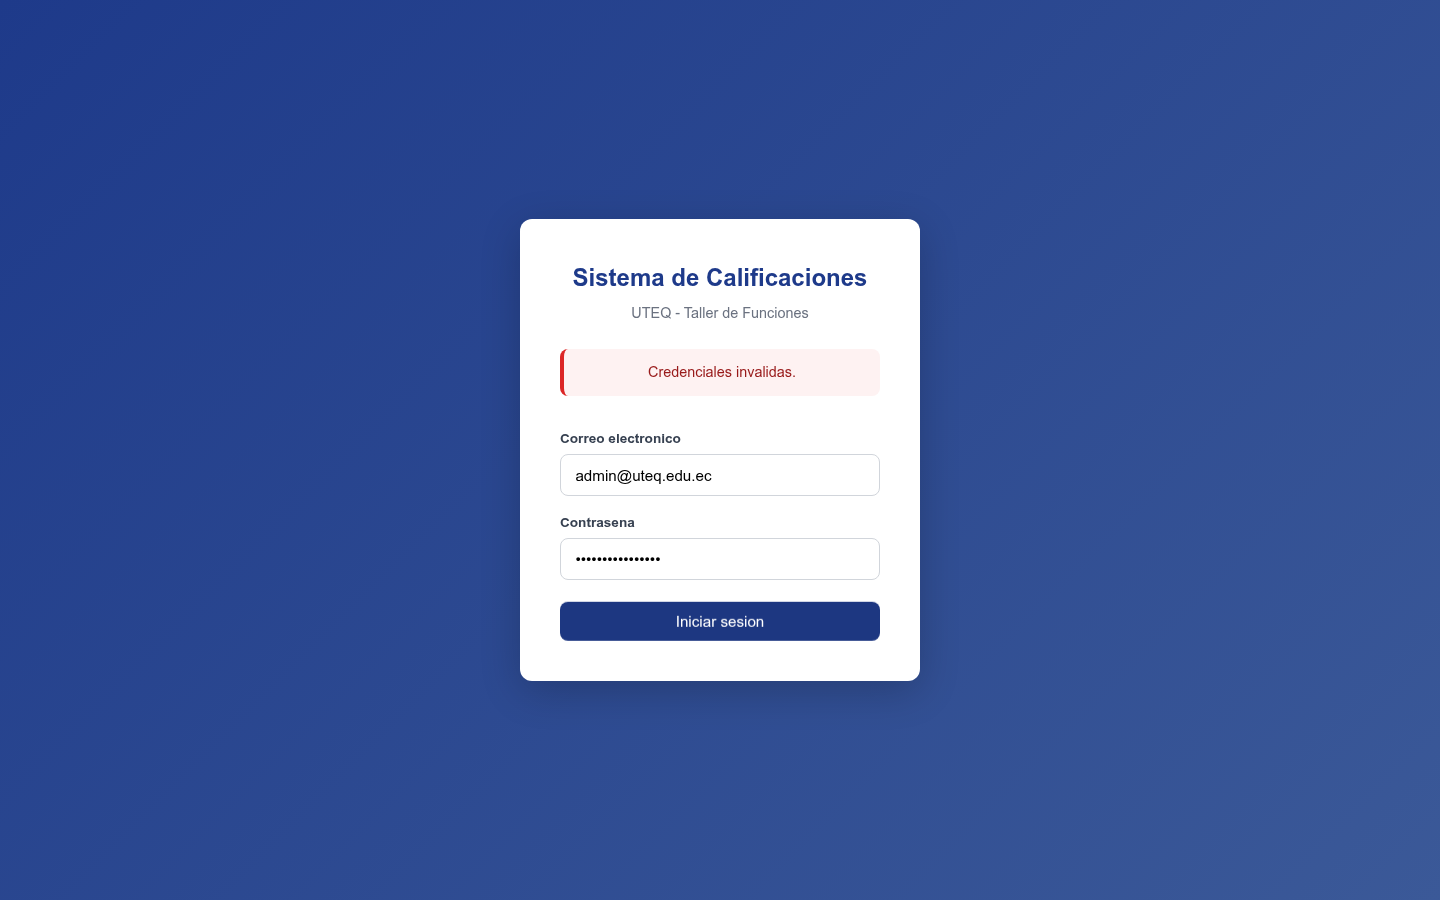
\includegraphics[width=0.92\textwidth]{evidencias/playwright-02-login-fallido.png}
\caption{Figura 7. Mensaje de error de credenciales inválidas (\texttt{playwright-02-login-fallido.png}).}
\end{figure}


\subsection*{5.4 CP-03 --- Registro de estudiante con cédula duplicada}
\addcontentsline{toc}{subsection}{5.4 CP-03 --- Registro de estudiante con cédula duplicada}


{\small
\begin{longtable}{|p{\dimexpr\textwidth/2-2\tabcolsep\relax}|p{\dimexpr\textwidth/2-2\tabcolsep\relax}|}
\rowcolor{UTECblue}\color{white}\bfseries Campo & \color{white}\bfseries Detalle \\ \hline
\endfirsthead
\rowcolor{UTECblue}\color{white}\bfseries Campo & \color{white}\bfseries Detalle \\ \hline
\endhead
Historia / Criterio & HU-02 / CA-3 \\ \hline
Precondiciones & Sesión de administrador; cédula \texttt{1250001111} ya registrada \\ \hline
Datos de prueba & \texttt{cedula=1250001111}, \texttt{nombres=Dup}, \texttt{apellidos=Test}, \texttt{fecha\_nacimiento=2010-01-01}, \texttt{id\_representante=1} \\ \hline
Pasos & Enviar \texttt{POST /api/estudiantes/} con la cédula duplicada \\ \hline
Resultado esperado & HTTP 409 con mensaje ''Ya existe un estudiante registrado con esa cedula.'' \\ \hline
Resultado obtenido & HTTP 409 + mensaje exacto \\ \hline
Estado & {\color{green!60!black}{$\checkmark$}} PASS \\ \hline
\end{longtable}}


\textbf{Evidencia (terminal):}


\subsection*{5.5 CP-04 --- Búsqueda de estudiante por cédula}
\addcontentsline{toc}{subsection}{5.5 CP-04 --- Búsqueda de estudiante por cédula}


{\small
\begin{longtable}{|p{\dimexpr\textwidth/2-2\tabcolsep\relax}|p{\dimexpr\textwidth/2-2\tabcolsep\relax}|}
\rowcolor{UTECblue}\color{white}\bfseries Campo & \color{white}\bfseries Detalle \\ \hline
\endfirsthead
\rowcolor{UTECblue}\color{white}\bfseries Campo & \color{white}\bfseries Detalle \\ \hline
\endhead
Historia / Criterio & HU-02 / CA-2 \\ \hline
Precondiciones & Sesión de administrador \\ \hline
Datos de prueba & \texttt{q=1250001111} \\ \hline
Pasos & 1) Ir a \texttt{estudiantes.html}. 2) Escribir la cédula en \texttt{\#q}. 3) Clic en Buscar. \\ \hline
Resultado esperado & Tabla con el estudiante buscado y su cédula \\ \hline
Resultado obtenido & Fila con la cédula y el nombre esperado \\ \hline
Estado & {\color{green!60!black}{$\checkmark$}} PASS \\ \hline
\end{longtable}}


\begin{figure}[H]
\centering
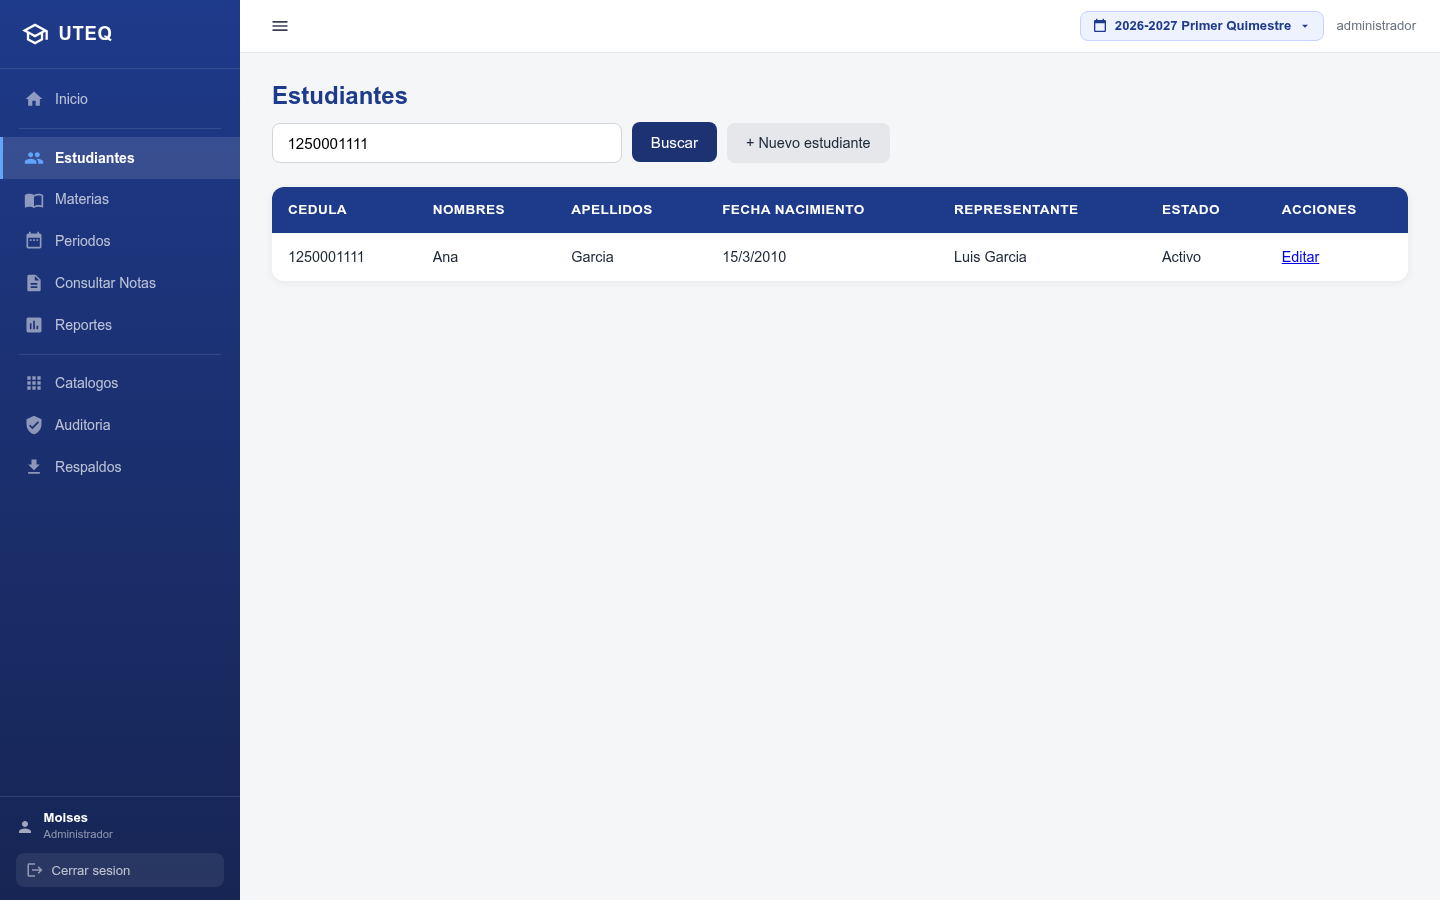
\includegraphics[width=0.92\textwidth]{evidencias/playwright-04-buscar-estudiante.png}
\caption{Figura 8. Búsqueda de estudiante por cédula (\texttt{playwright-04-buscar-estudiante.png}).}
\end{figure}


\subsection*{5.6 CP-05 {$\star$} --- Registro de calificaciones en rango válido (guardado masivo)}
\addcontentsline{toc}{subsection}{5.6 CP-05 {$\star$} --- Registro de calificaciones en rango válido (guardado masivo)}


{\small
\begin{longtable}{|p{\dimexpr\textwidth/2-2\tabcolsep\relax}|p{\dimexpr\textwidth/2-2\tabcolsep\relax}|}
\rowcolor{UTECblue}\color{white}\bfseries Campo & \color{white}\bfseries Detalle \\ \hline
\endfirsthead
\rowcolor{UTECblue}\color{white}\bfseries Campo & \color{white}\bfseries Detalle \\ \hline
\endhead
Historia / Criterio & HU-03 / CA-1, CA-3 \\ \hline
Precondiciones & Sesión de Elena Romero (profesora de ''Ciencias Naturales''); periodo activo = 1 \\ \hline
Datos de prueba & Materia: Ciencias Naturales; nota: 8.75 \\ \hline
Pasos & 1) Ir a \texttt{calificaciones.html}. 2) Seleccionar la materia. 3) Ingresar la nota 8.75. 4) ''Guardar todas''. \\ \hline
Resultado esperado & Mensaje de éxito ''Se guardaron N calificaciones.'' \\ \hline
Resultado obtenido & \texttt{\#ok} visible con ''Se guardaron 1 calificaciones.'' \\ \hline
Estado & {\color{green!60!black}{$\checkmark$}} PASS \\ \hline
\end{longtable}}


\begin{figure}[H]
\centering
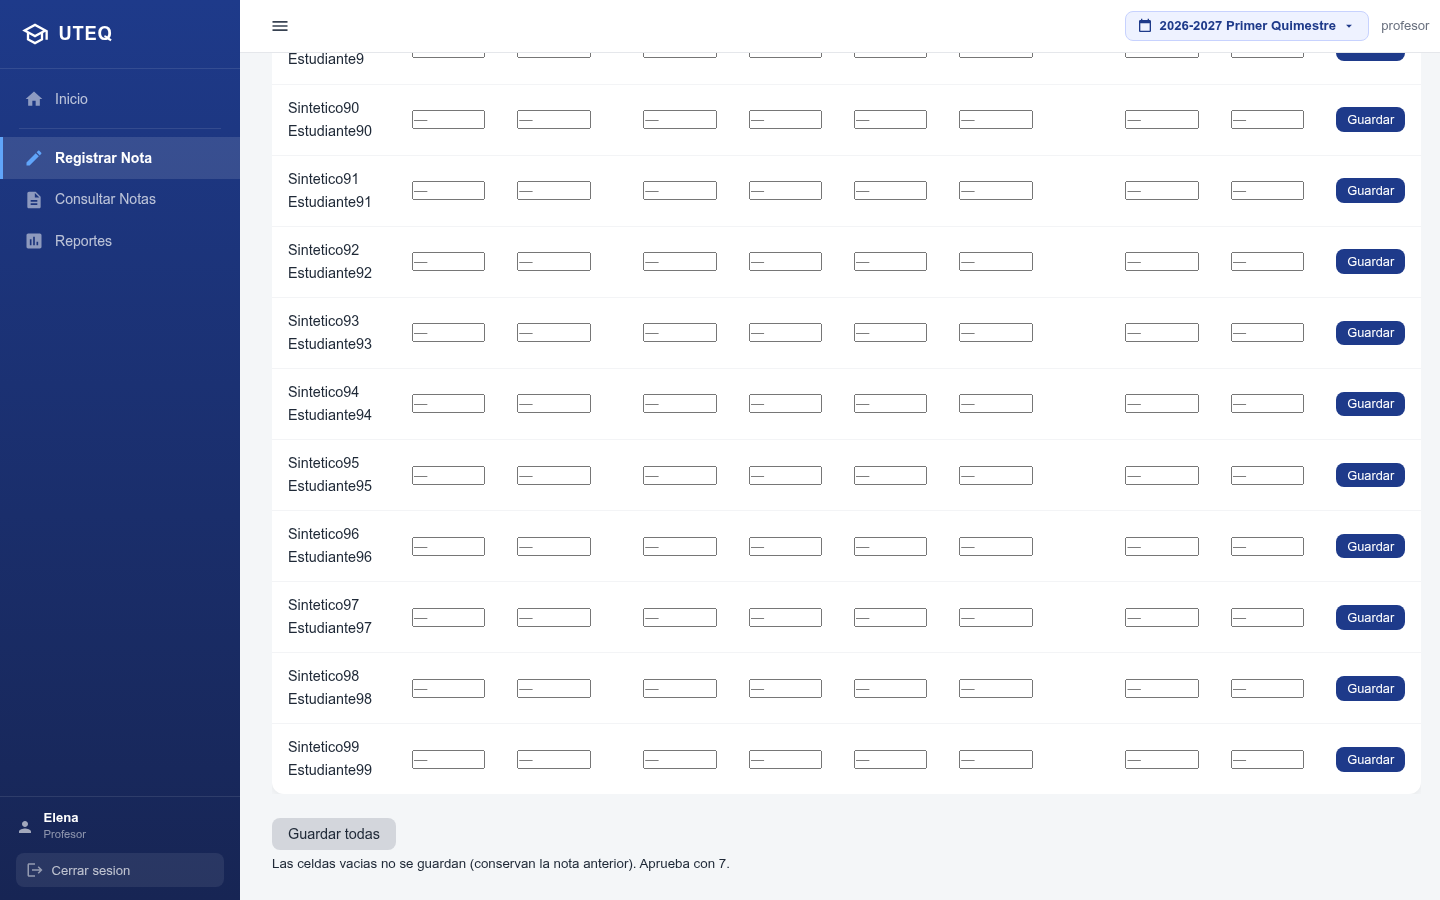
\includegraphics[width=0.92\textwidth]{evidencias/playwright-05-profesor-notas.png}
\caption{Figura 9. Registro de calificaciones del profesor (\texttt{playwright-05-profesor-notas.png}).}
\end{figure}


\subsection*{5.7 CP-06 --- Nota fuera de rango (0--10) rechazada}
\addcontentsline{toc}{subsection}{5.7 CP-06 --- Nota fuera de rango (0--10) rechazada}


{\small
\begin{longtable}{|p{\dimexpr\textwidth/2-2\tabcolsep\relax}|p{\dimexpr\textwidth/2-2\tabcolsep\relax}|}
\rowcolor{UTECblue}\color{white}\bfseries Campo & \color{white}\bfseries Detalle \\ \hline
\endfirsthead
\rowcolor{UTECblue}\color{white}\bfseries Campo & \color{white}\bfseries Detalle \\ \hline
\endhead
Historia / Criterio & HU-03 / CA-2 \\ \hline
Precondiciones & Sesión de Elena Romero \\ \hline
Datos de prueba & \texttt{valor=11}, materia 3, periodo 1, estudiante 1, tipo 1 \\ \hline
Pasos & Enviar \texttt{POST /api/calificaciones/} con valor 11 \\ \hline
Resultado esperado & HTTP 400: ''La calificacion 11 esta fuera de rango (0 a 10)'' \\ \hline
Resultado obtenido & HTTP 400 + mensaje exacto (validado en SP y trigger) \\ \hline
Estado & {\color{green!60!black}{$\checkmark$}} PASS \\ \hline
\end{longtable}}


\textbf{Evidencia (terminal):}


\subsection*{5.8 CP-07 {$\star$} --- Profesor bloqueado para materia no asignada}
\addcontentsline{toc}{subsection}{5.8 CP-07 {$\star$} --- Profesor bloqueado para materia no asignada}


{\small
\begin{longtable}{|p{\dimexpr\textwidth/2-2\tabcolsep\relax}|p{\dimexpr\textwidth/2-2\tabcolsep\relax}|}
\rowcolor{UTECblue}\color{white}\bfseries Campo & \color{white}\bfseries Detalle \\ \hline
\endfirsthead
\rowcolor{UTECblue}\color{white}\bfseries Campo & \color{white}\bfseries Detalle \\ \hline
\endhead
Historia / Criterio & HU-03 / CA-5 \\ \hline
Precondiciones & Sesión de Elena Romero (solo tiene ''Ciencias Naturales'', id 3) \\ \hline
Datos de prueba & \texttt{id\_materia=1} (Matemáticas), periodo 1, valor 8.5 \\ \hline
Pasos & Enviar \texttt{POST /api/calificaciones/} intentando registrar en Matemáticas \\ \hline
Resultado esperado & HTTP 403: ''No tiene asignada esta materia en el periodo: no puede registrar la nota.'' \\ \hline
Resultado obtenido & HTTP 403 + mensaje exacto \\ \hline
Estado & {\color{green!60!black}{$\checkmark$}} PASS \\ \hline
\end{longtable}}


\textbf{Evidencia (terminal):}


\subsection*{5.9 CP-08 --- Consulta de notas (representante)}
\addcontentsline{toc}{subsection}{5.9 CP-08 --- Consulta de notas (representante)}


{\small
\begin{longtable}{|p{\dimexpr\textwidth/2-2\tabcolsep\relax}|p{\dimexpr\textwidth/2-2\tabcolsep\relax}|}
\rowcolor{UTECblue}\color{white}\bfseries Campo & \color{white}\bfseries Detalle \\ \hline
\endfirsthead
\rowcolor{UTECblue}\color{white}\bfseries Campo & \color{white}\bfseries Detalle \\ \hline
\endhead
Historia / Criterio & HU-04 / CA-1, CA-2, CA-3 \\ \hline
Precondiciones & Sesión de Fernando Castillo (representante) \\ \hline
Datos de prueba & Hijo: Isabella Castillo \\ \hline
Pasos & 1) Ir a \texttt{consulta.html}. 2) Seleccionar el estudiante. 3) Verificar notas, promedio y escala \\ \hline
Resultado esperado & Tablas de notas por materia, promedio general y escala cualitativa \\ \hline
Resultado obtenido & Tabla con notas y ''Promedio'' visibles; solo datos del hijo del representante \\ \hline
Estado & {\color{green!60!black}{$\checkmark$}} PASS \\ \hline
\end{longtable}}


\begin{figure}[H]
\centering
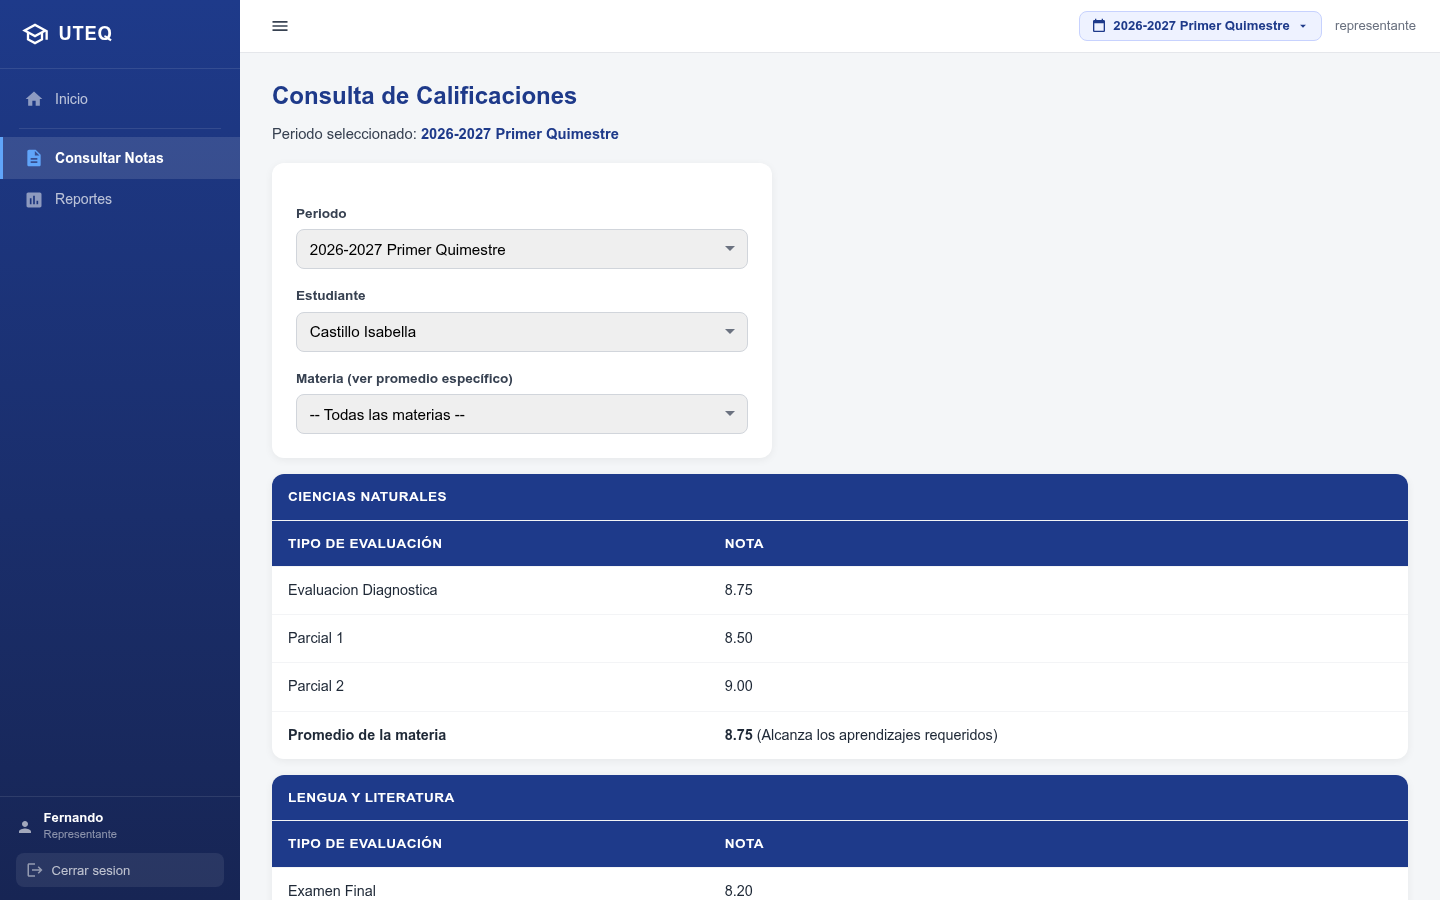
\includegraphics[width=0.92\textwidth]{evidencias/playwright-06-representante-consulta.png}
\caption{Figura 10. Consulta de calificaciones del representante (\texttt{playwright-06-representante-consulta.png}).}
\end{figure}


\subsection*{5.10 CP-09 {$\star$} --- Reporte de promedios por periodo}
\addcontentsline{toc}{subsection}{5.10 CP-09 {$\star$} --- Reporte de promedios por periodo}


{\small
\begin{longtable}{|p{\dimexpr\textwidth/2-2\tabcolsep\relax}|p{\dimexpr\textwidth/2-2\tabcolsep\relax}|}
\rowcolor{UTECblue}\color{white}\bfseries Campo & \color{white}\bfseries Detalle \\ \hline
\endfirsthead
\rowcolor{UTECblue}\color{white}\bfseries Campo & \color{white}\bfseries Detalle \\ \hline
\endhead
Historia / Criterio & HU-05 / CA-1, CA-3 \\ \hline
Precondiciones & Sesión con permisos (admin) \\ \hline
Datos de prueba & \texttt{id\_periodo=1} (periodo activo) \\ \hline
Pasos & Enviar \texttt{GET /api/reportes/?id\_periodo=1} \\ \hline
Resultado esperado & Lista ordenada por promedio descendente con escala cualitativa \\ \hline
Resultado obtenido & 10 filas; Top 3: Daniel 9.22 {$\cdot$} Sofía 9.10 {$\cdot$} Camila 9.03; escala ''Domina los aprendizajes requeridos'' \\ \hline
Estado & {\color{green!60!black}{$\checkmark$}} PASS \\ \hline
\end{longtable}}


\textbf{Evidencia (terminal):}


\subsection*{5.11 CP-10 --- Panel de auditoría (admin)}
\addcontentsline{toc}{subsection}{5.11 CP-10 --- Panel de auditoría (admin)}


{\small
\begin{longtable}{|p{\dimexpr\textwidth/2-2\tabcolsep\relax}|p{\dimexpr\textwidth/2-2\tabcolsep\relax}|}
\rowcolor{UTECblue}\color{white}\bfseries Campo & \color{white}\bfseries Detalle \\ \hline
\endfirsthead
\rowcolor{UTECblue}\color{white}\bfseries Campo & \color{white}\bfseries Detalle \\ \hline
\endhead
Historia / Criterio & HU-06 / CA-1 a CA-4 \\ \hline
Precondiciones & Sesión de administrador; actividad registrada \\ \hline
Datos de prueba & \texttt{page=1\&limit=3} \\ \hline
Pasos & 1) Ir a \texttt{auditoria.html}. 2) Verificar total, filtros y registros con JSONB antes/después \\ \hline
Resultado esperado & Total > 0; registros con \texttt{datos\_anteriores}/\texttt{datos\_nuevos} y usuario de la app \\ \hline
Resultado obtenido & Panel con total de registros; filtros por fecha y categoría; detalle JSONB \\ \hline
Estado & {\color{green!60!black}{$\checkmark$}} PASS \\ \hline
\end{longtable}}


\begin{figure}[H]
\centering
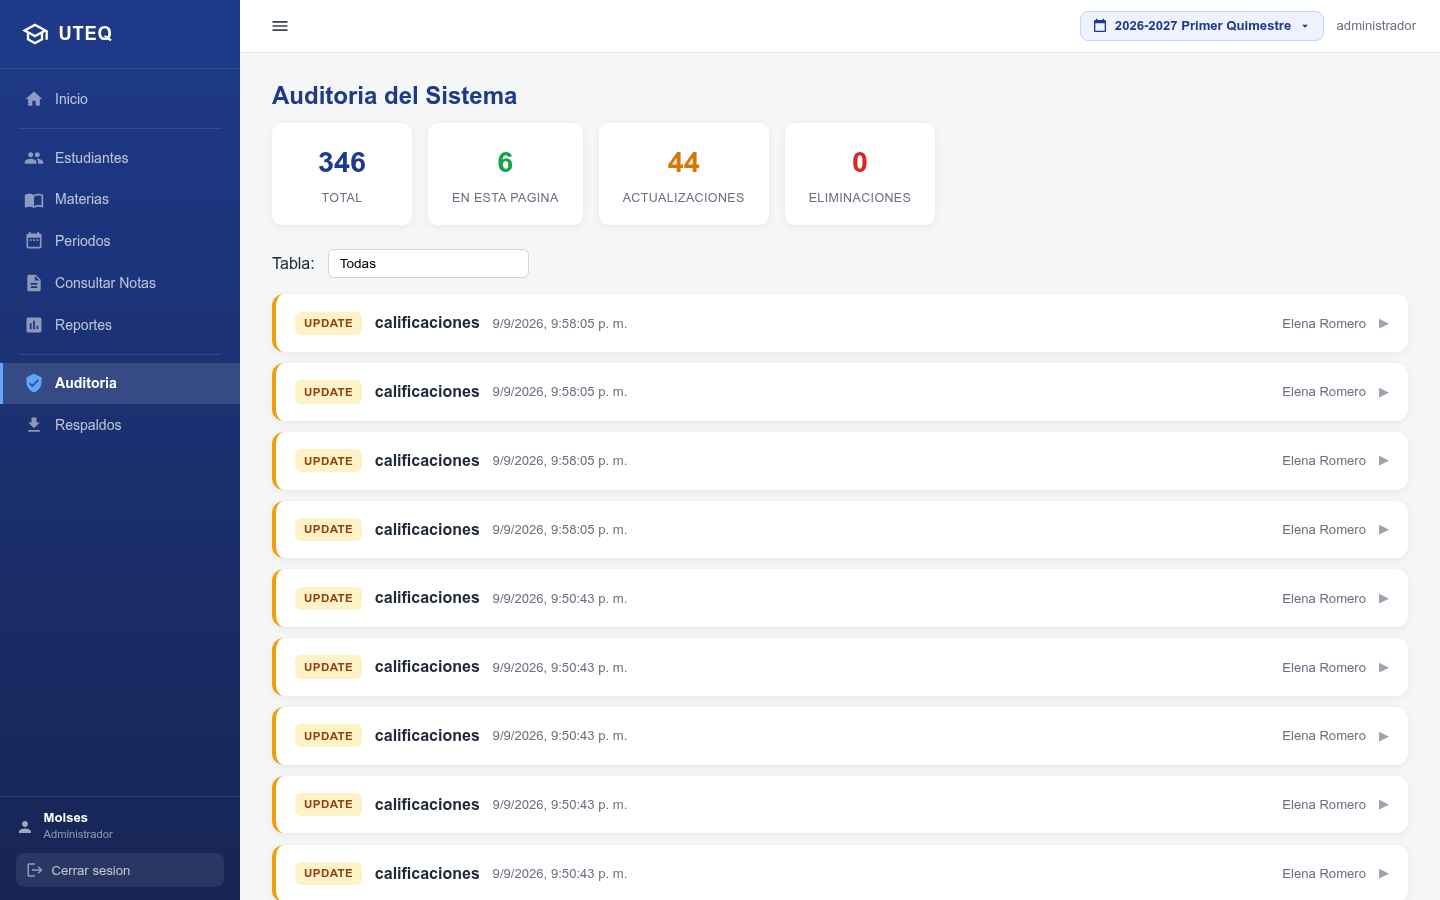
\includegraphics[width=0.92\textwidth]{evidencias/playwright-03-admin-auditoria.png}
\caption{Figura 11. Panel de auditoría del administrador (\texttt{playwright-03-admin-auditoria.png}).}
\end{figure}


\textbf{Verificación de API:} \texttt{GET /api/auditoria/?page=1\&limit=3} {$\rightarrow$} total acumulado creciente (en la corrida de evidencias, 1117 registros); la suite \texttt{e2e\_test.js} verifica además que cada fila contenga el usuario de la aplicación y que Elena (profesor) reciba 403 al intentar acceder.


\subsection*{5.12 CP-11 --- Restricción de acceso a auditoría/respaldos (no admin)}
\addcontentsline{toc}{subsection}{5.12 CP-11 --- Restricción de acceso a auditoría/respaldos (no admin)}


{\small
\begin{longtable}{|p{\dimexpr\textwidth/2-2\tabcolsep\relax}|p{\dimexpr\textwidth/2-2\tabcolsep\relax}|}
\rowcolor{UTECblue}\color{white}\bfseries Campo & \color{white}\bfseries Detalle \\ \hline
\endfirsthead
\rowcolor{UTECblue}\color{white}\bfseries Campo & \color{white}\bfseries Detalle \\ \hline
\endhead
Historia / Criterio & HU-06 / CA-1, HU-08 / CA-3 \\ \hline
Precondiciones & Sesión de representante y de profesor \\ \hline
Datos de prueba & Sesión de Fernando Castillo (representante) \\ \hline
Pasos & 1) Verificar que el menú no muestra Auditoría/Respaldos. 2) Navegar directo por URL a \texttt{auditoria.html} \\ \hline
Resultado esperado & Error ''No tienes permiso para acceder a esta seccion.'' \\ \hline
Resultado obtenido & Mensaje de permiso denegado en \texttt{main .alert-error} \\ \hline
Estado & {\color{green!60!black}{$\checkmark$}} PASS \\ \hline
\end{longtable}}


\begin{figure}[H]
\centering
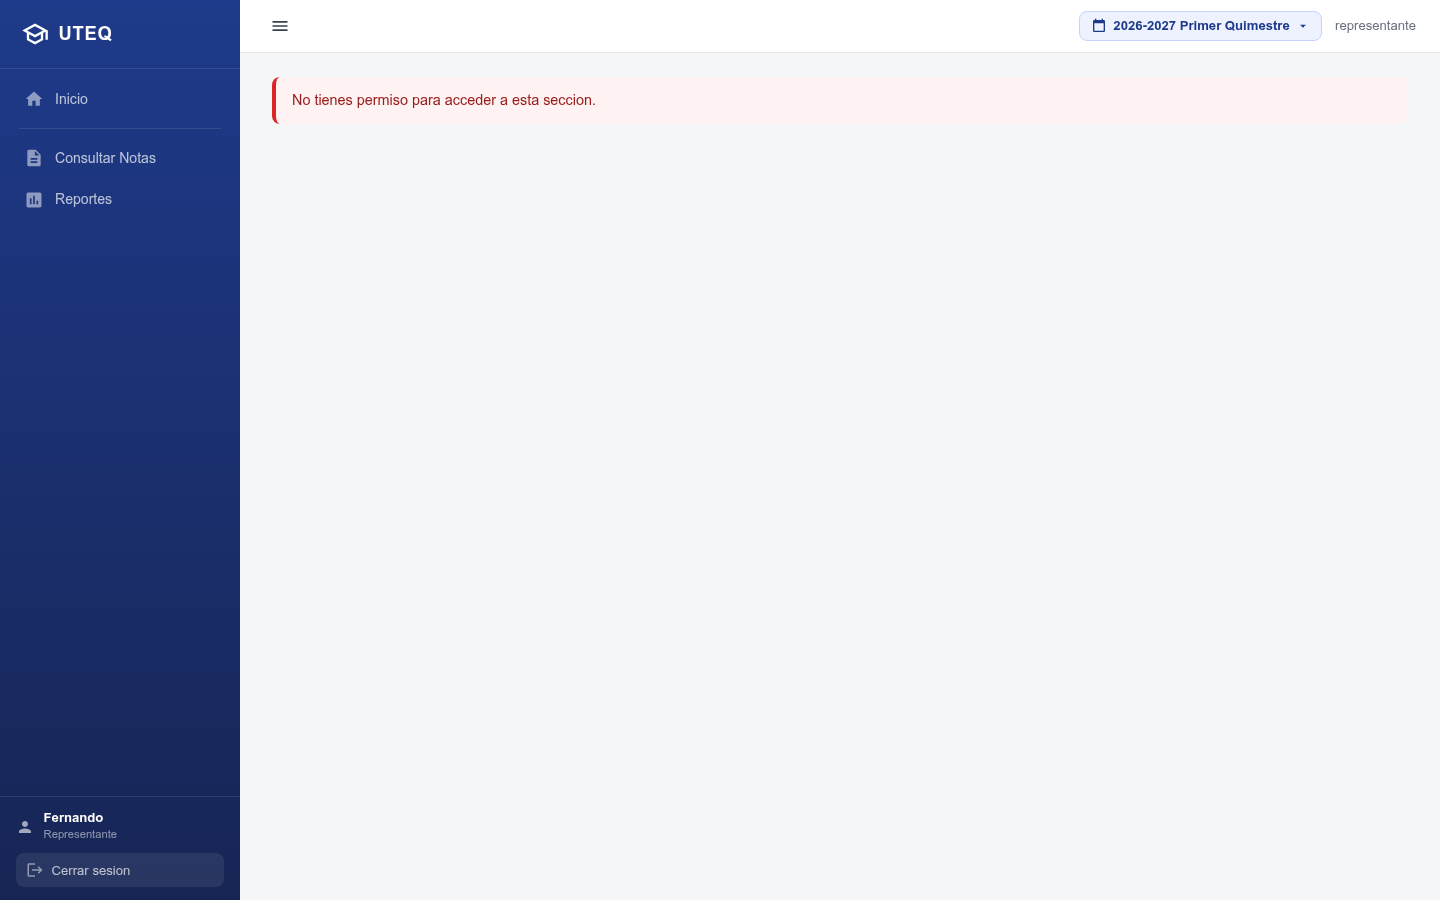
\includegraphics[width=0.92\textwidth]{evidencias/playwright-07-acceso-denegado.png}
\caption{Figura 12. Control de acceso: mensaje de permiso denegado (\texttt{playwright-07-acceso-denegado.png}).}
\end{figure}


\subsection*{5.13 CP-12 --- Creación de periodo con fechas inválidas rechazada}
\addcontentsline{toc}{subsection}{5.13 CP-12 --- Creación de periodo con fechas inválidas rechazada}


{\small
\begin{longtable}{|p{\dimexpr\textwidth/2-2\tabcolsep\relax}|p{\dimexpr\textwidth/2-2\tabcolsep\relax}|}
\rowcolor{UTECblue}\color{white}\bfseries Campo & \color{white}\bfseries Detalle \\ \hline
\endfirsthead
\rowcolor{UTECblue}\color{white}\bfseries Campo & \color{white}\bfseries Detalle \\ \hline
\endhead
Historia / Criterio & HU-07 / CA-1, CA-2 \\ \hline
Precondiciones & Sesión de administrador \\ \hline
Datos de prueba & \texttt{nombre=Test}, inicio 2026-09-01, fin 2026-01-01 \\ \hline
Pasos & Enviar \texttt{POST /api/periodos/} con fecha de fin anterior a la fecha de inicio \\ \hline
Resultado esperado & HTTP 400: ''La fecha de fin debe ser posterior a la fecha de inicio.'' \\ \hline
Resultado obtenido & HTTP 400 + mensaje exacto (CHECK en BD + validación en ruta) \\ \hline
Estado & {\color{green!60!black}{$\checkmark$}} PASS \\ \hline
\end{longtable}}


\textbf{Evidencia (terminal):}


\subsection*{5.14 CP-13 --- Rendimiento académico (psicóloga)}
\addcontentsline{toc}{subsection}{5.14 CP-13 --- Rendimiento académico (psicóloga)}


{\small
\begin{longtable}{|p{\dimexpr\textwidth/2-2\tabcolsep\relax}|p{\dimexpr\textwidth/2-2\tabcolsep\relax}|}
\rowcolor{UTECblue}\color{white}\bfseries Campo & \color{white}\bfseries Detalle \\ \hline
\endfirsthead
\rowcolor{UTECblue}\color{white}\bfseries Campo & \color{white}\bfseries Detalle \\ \hline
\endhead
Historia / Criterio & HU-09 / CA-1 a CA-3 \\ \hline
Precondiciones & Sesión de María Torres (psicóloga) \\ \hline
Datos de prueba & Estudiantes del periodo activo \\ \hline
Pasos & 1) Ir a \texttt{psicologo.html}. 2) Ver resumen y alertas. 3) Abrir el detalle de un estudiante \\ \hline
Resultado esperado & Resumen de tarjetas, alertas y detalle por estudiante \\ \hline
Resultado obtenido & \texttt{\#resumen} visible; la API \texttt{/psicologo/rendimiento} devuelve resumen (total, alertas, promedios) y el detalle por estudiante \\ \hline
Estado & {\color{green!60!black}{$\checkmark$}} PASS \\ \hline
\end{longtable}}


\begin{figure}[H]
\centering
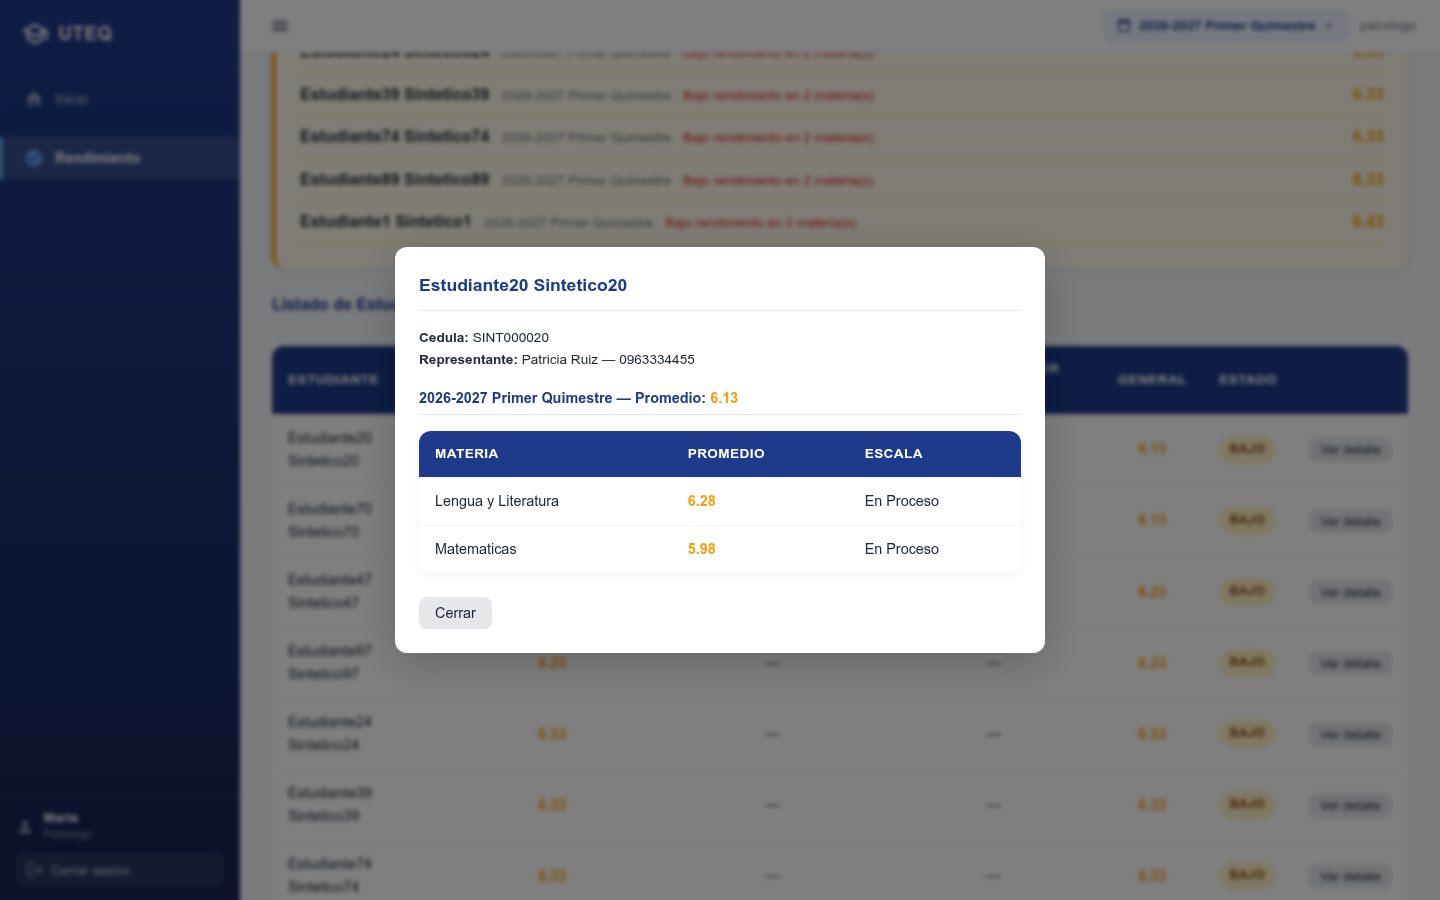
\includegraphics[width=0.92\textwidth]{evidencias/playwright-08-psicologo.png}
\caption{Figura 13. Panel de rendimiento de la psicóloga (\texttt{playwright-08-psicologo.png}).}
\end{figure}


\subsection*{5.15 CP-14 --- Cierre de sesión}
\addcontentsline{toc}{subsection}{5.15 CP-14 --- Cierre de sesión}


{\small
\begin{longtable}{|p{\dimexpr\textwidth/2-2\tabcolsep\relax}|p{\dimexpr\textwidth/2-2\tabcolsep\relax}|}
\rowcolor{UTECblue}\color{white}\bfseries Campo & \color{white}\bfseries Detalle \\ \hline
\endfirsthead
\rowcolor{UTECblue}\color{white}\bfseries Campo & \color{white}\bfseries Detalle \\ \hline
\endhead
Historia / Criterio & HU-01 / CA-1 (cierre) \\ \hline
Precondiciones & Sesión iniciada \\ \hline
Pasos & 1) Clic en \texttt{\#btn-logout} \\ \hline
Resultado esperado & Redirección a \texttt{login.html} y sesión destruida \\ \hline
Resultado obtenido & Redirección correcta y formulario de login visible \\ \hline
Estado & {\color{green!60!black}{$\checkmark$}} PASS \\ \hline
\end{longtable}}


\begin{figure}[H]
\centering
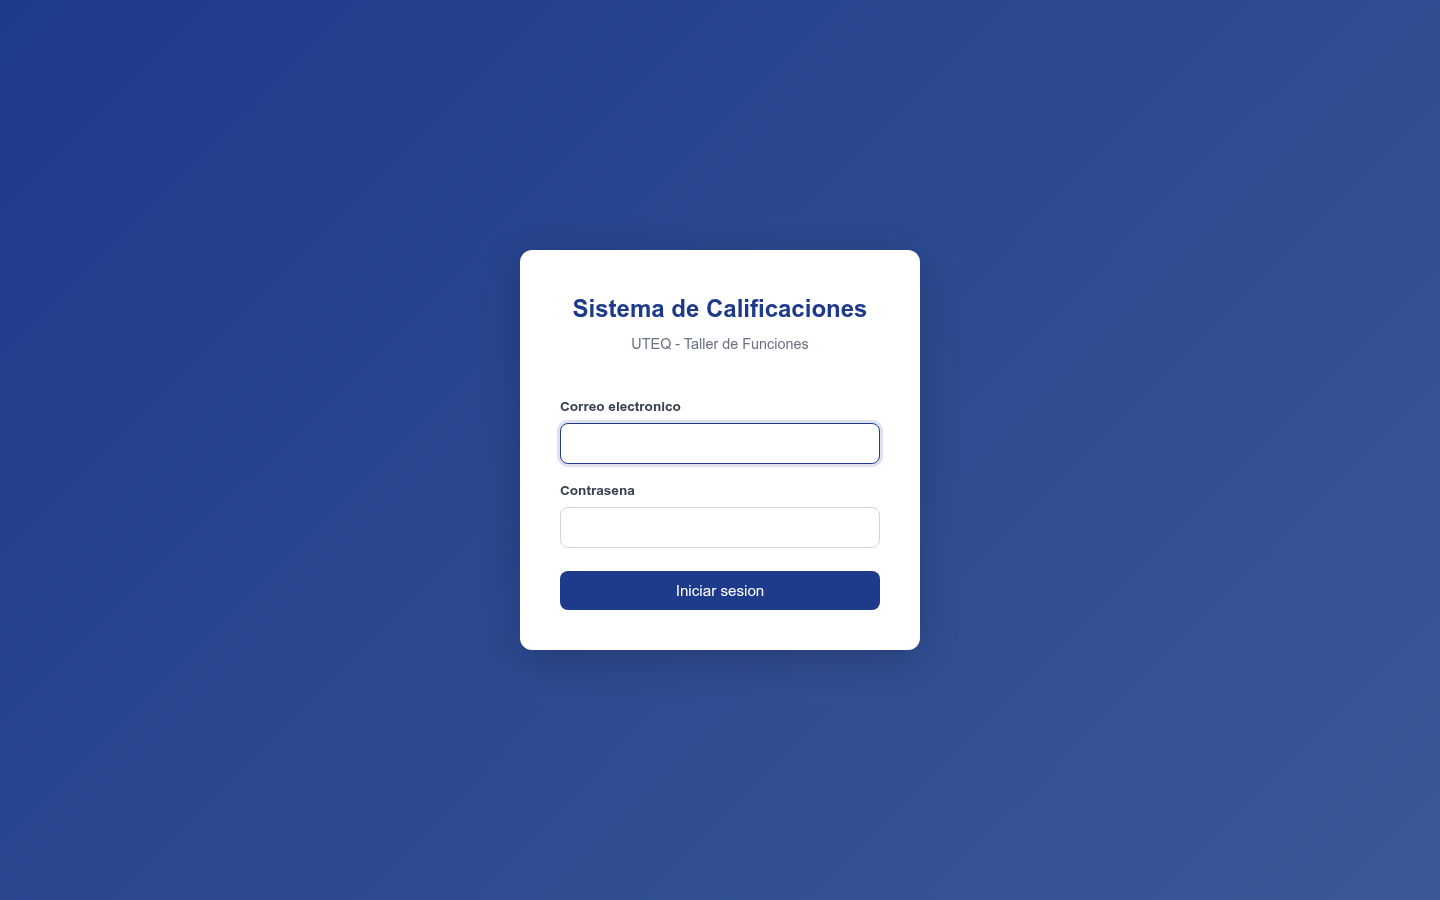
\includegraphics[width=0.92\textwidth]{evidencias/playwright-09-logout.png}
\caption{Figura 14. Cierre de sesión y retorno al login (\texttt{playwright-09-logout.png}).}
\end{figure}


\subsection*{5.16 Técnicas de diseño de casos aplicadas}
\addcontentsline{toc}{subsection}{5.16 Técnicas de diseño de casos aplicadas}


Cada caso manual se diseñó con una técnica explícita para garantizar su valor de detección:


{\small
\begin{longtable}{|p{\dimexpr\textwidth/2-2\tabcolsep\relax}|p{\dimexpr\textwidth/2-2\tabcolsep\relax}|}
\rowcolor{UTECblue}\color{white}\bfseries Técnica & \color{white}\bfseries Aplicación en el plan de pruebas \\ \hline
\endfirsthead
\rowcolor{UTECblue}\color{white}\bfseries Técnica & \color{white}\bfseries Aplicación en el plan de pruebas \\ \hline
\endhead
Partición de equivalencia & Rango de notas (válido 0--10 / inválido 11); cédula (única / duplicada); fechas de periodo (inicio < fin / inicio {$\geq$} fin) \\ \hline
Valores límite & Extremos del rango 0 y 10 aceptados; 11 y -1 rechazados; página de 10 elementos \\ \hline
Transiciones de estado & Login (sin sesión {$\rightarrow$} dashboard {$\rightarrow$} logout); cambio de periodo activo; activación de un único periodo \\ \hline
Prueba negativa & 403 de materia no asignada, 403 de auditoría a no-admin, 400 de categoría de auditoría inválida, 409 de asignación duplicada \\ \hline
Tabla de decisión & Evaluación de la escala cualitativa según el promedio (4 rangos) \\ \hline
Recorrido por casos de uso & Flujos completos: registro masivo de notas, consulta de representante, panel de psicóloga \\ \hline
\end{longtable}}


\subsection*{5.17 Matriz de trazabilidad de los casos manuales}
\addcontentsline{toc}{subsection}{5.17 Matriz de trazabilidad de los casos manuales}


{\small
\begin{longtable}{|p{\dimexpr\textwidth/5-2\tabcolsep\relax}|p{\dimexpr\textwidth/5-2\tabcolsep\relax}|p{\dimexpr\textwidth/5-2\tabcolsep\relax}|p{\dimexpr\textwidth/5-2\tabcolsep\relax}|p{\dimexpr\textwidth/5-2\tabcolsep\relax}|}
\rowcolor{UTECblue}\color{white}\bfseries Caso & \color{white}\bfseries Historia & \color{white}\bfseries Técnica principal & \color{white}\bfseries Resultado & \color{white}\bfseries Evidencia \\ \hline
\endfirsthead
\rowcolor{UTECblue}\color{white}\bfseries Caso & \color{white}\bfseries Historia & \color{white}\bfseries Técnica principal & \color{white}\bfseries Resultado & \color{white}\bfseries Evidencia \\ \hline
\endhead
CP-01 & HU-01 & Caso de uso & {\color{green!60!black}{$\checkmark$}} PASS & playwright-01 \\ \hline
CP-02 & HU-01 & Prueba negativa & {\color{green!60!black}{$\checkmark$}} PASS & playwright-02 \\ \hline
CP-03 & HU-02 & Partición & {\color{green!60!black}{$\checkmark$}} PASS & pruebas\_api\_manuales.txt \\ \hline
CP-04 & HU-02 & Caso de uso & {\color{green!60!black}{$\checkmark$}} PASS & playwright-04 \\ \hline
CP-05 & HU-03 & Valores límite & {\color{green!60!black}{$\checkmark$}} PASS & playwright-05 \\ \hline
CP-06 & HU-03 & Valores límite & {\color{green!60!black}{$\checkmark$}} PASS & pruebas\_api\_manuales.txt \\ \hline
CP-07 & HU-03 & Prueba negativa & {\color{green!60!black}{$\checkmark$}} PASS & pruebas\_api\_manuales.txt \\ \hline
CP-08 & HU-04 & Caso de uso & {\color{green!60!black}{$\checkmark$}} PASS & playwright-06 \\ \hline
CP-09 & HU-05 & Tabla de decisión & {\color{green!60!black}{$\checkmark$}} PASS & pruebas\_api\_manuales.txt \\ \hline
CP-10 & HU-06 & Recorrido & {\color{green!60!black}{$\checkmark$}} PASS & playwright-03 + e2e \\ \hline
CP-11 & HU-06/HU-08 & Prueba negativa & {\color{green!60!black}{$\checkmark$}} PASS & playwright-07 \\ \hline
CP-12 & HU-07 & Partición & {\color{green!60!black}{$\checkmark$}} PASS & pruebas\_api\_manuales.txt \\ \hline
CP-13 & HU-09 & Recorrido & {\color{green!60!black}{$\checkmark$}} PASS & playwright-08 \\ \hline
CP-14 & HU-01 & Transición & {\color{green!60!black}{$\checkmark$}} PASS & playwright-09 \\ \hline
\end{longtable}}


\subsection*{5.18 Pruebas complementarias}
\addcontentsline{toc}{subsection}{5.18 Pruebas complementarias}


Además de los casos funcionales, se ejecutaron pruebas complementarias que refuerzan la calidad del sistema:


\begin{enumerate}[leftmargin=*]
\item \textbf{Compatibilidad de navegadores:} las pantallas principales (login, consulta y auditoría) se verificaron en Chrome y Edge, tanto en escritorio como en vista móvil emulada. No se detectaron diferencias de comportamiento.
\item \textbf{Respaldo y restauración:} se generó un respaldo manual con \texttt{pg\_dump} desde el panel (archivo \texttt{respaldo\_*.sql}), se listó en el historial y se restauró sobre una base vacía para confirmar la integridad del ciclo de respaldo. Verificado por la suite API (sección 8 de los checks).
\item \textbf{Seguridad básica:} se comprobó que las contraseñas se almacenan con bcrypt, que la sesión usa cookie firmada y se destruye al cerrar sesión (CP-14), y que las rutas sensibles rechazan a roles no autorizados con HTTP 403 (CP-07, CP-11 y sección 9 de los checks de API).
\item \textbf{Cierre de sesión:} comprobado tanto en UI (CP-14) como por API (sin sesión {$\rightarrow$} redirección al login en \texttt{auth.spec.cjs}).
\end{enumerate}


\subsection*{5.19 Resumen de ejecución}
\addcontentsline{toc}{subsection}{5.19 Resumen de ejecución}


\textbf{Tabla 5. Resumen de casos de prueba manuales.}


{\small
\begin{longtable}{|p{\dimexpr\textwidth/4-2\tabcolsep\relax}|p{\dimexpr\textwidth/4-2\tabcolsep\relax}|p{\dimexpr\textwidth/4-2\tabcolsep\relax}|p{\dimexpr\textwidth/4-2\tabcolsep\relax}|}
\rowcolor{UTECblue}\color{white}\bfseries Total & \color{white}\bfseries PASS & \color{white}\bfseries FAIL & \color{white}\bfseries Evidencias \\ \hline
\endfirsthead
\rowcolor{UTECblue}\color{white}\bfseries Total & \color{white}\bfseries PASS & \color{white}\bfseries FAIL & \color{white}\bfseries Evidencias \\ \hline
\endhead
\end{longtable}}


Los casos marcados con {$\star$} (CP-05, CP-07 y CP-09) son los seleccionados para la demostración en vivo: cubren tres módulos distintos y combinan flujo positivo, negativo y cálculo.


{\small
\begin{longtable}{|p{\dimexpr\textwidth/4-2\tabcolsep\relax}|p{\dimexpr\textwidth/4-2\tabcolsep\relax}|p{\dimexpr\textwidth/4-2\tabcolsep\relax}|p{\dimexpr\textwidth/4-2\tabcolsep\relax}|}
\rowcolor{UTECblue}\color{white}\bfseries 14 & \color{white}\bfseries 14 & \color{white}\bfseries 0 & \color{white}\bfseries 9 capturas Playwright + \texttt{pruebas\_api\_manuales.txt} + suites del repositorio (66 API + 35 UI) \\ \hline
\endfirsthead
\rowcolor{UTECblue}\color{white}\bfseries 14 & \color{white}\bfseries 14 & \color{white}\bfseries 0 & \color{white}\bfseries 9 capturas Playwright + \texttt{pruebas\_api\_manuales.txt} + suites del repositorio (66 API + 35 UI) \\ \hline
\endhead
\end{longtable}}


\section*{6. Automatización de pruebas (API y UI)}
\addcontentsline{toc}{section}{6. Automatización de pruebas (API y UI)}


\subsection*{6.1 Herramientas y configuración}
\addcontentsline{toc}{subsection}{6.1 Herramientas y configuración}


Se automatizaron \textbf{dos niveles} de prueba, alineados con el Plan de Mejoras v2 del repositorio (Fases 1--8):


\begin{enumerate}[leftmargin=*]
\item \textbf{Nivel API (back-end):} script \texttt{backend/e2e\_test.js} ejecutado con \texttt{npm test}. Cubre auth por rol, calificaciones con parcial/ciclo, auditoría, paginación, CRUD de catálogos con 409/400/403, respaldos con log, consulta por bloques, representantes, dashboards por rol y control de acceso. Resultado: \textbf{66/66 PASS}.
\item \textbf{Nivel UI (front-end):} suite \textbf{Playwright} en \texttt{backend/tests/e2e/} (10 archivos de spec). Resultado: \textbf{35/35 PASS}.
\end{enumerate}


{\small
\begin{longtable}{|p{\dimexpr\textwidth/2-2\tabcolsep\relax}|p{\dimexpr\textwidth/2-2\tabcolsep\relax}|}
\rowcolor{UTECblue}\color{white}\bfseries Elemento & \color{white}\bfseries Detalle \\ \hline
\endfirsthead
\rowcolor{UTECblue}\color{white}\bfseries Elemento & \color{white}\bfseries Detalle \\ \hline
\endhead
Framework UI & \texttt{@playwright/test} (\textasciicircum{}1.63.0), navegador Chromium \\ \hline
Configuración & \texttt{backend/tests/playwright.config.js} \\ \hline
Base URL & \texttt{\url{http://localhost:3000}} (API + frontend estático, mismo origen) \\ \hline
Ejecución API & \texttt{npm test} (desde \texttt{backend/}) \\ \hline
Ejecución UI & \texttt{npm run test:e2e} (desde \texttt{backend/}) \\ \hline
Reporter UI & HTML (\texttt{report/}) + list \\ \hline
Modo de ejecución & Serializado (\texttt{workers: 1}) por base de datos compartida \\ \hline
\end{longtable}}


\textbf{Contenido de \texttt{backend/tests/playwright.config.js}:}


\subsection*{6.2 Nivel API --- los 66 checks}
\addcontentsline{toc}{subsection}{6.2 Nivel API --- los 66 checks}


\textbf{Tabla 6. Clasificación de los 66 checks de API.}


{\small
\begin{longtable}{|p{\dimexpr\textwidth/2-2\tabcolsep\relax}|p{\dimexpr\textwidth/2-2\tabcolsep\relax}|}
\rowcolor{UTECblue}\color{white}\bfseries Área & \color{white}\bfseries Alcance \\ \hline
\endfirsthead
\rowcolor{UTECblue}\color{white}\bfseries Área & \color{white}\bfseries Alcance \\ \hline
\endhead
Auth (5 roles) & Login admin/profesor({$\times$}2)/representante/psicóloga {$\cdot$} password incorrecta {$\cdot$} acceso sin sesión \\ \hline
Calificaciones & Contexto usable {$\cdot$} parcial/ciclo {$\cdot$} lote con upsert {$\cdot$} verificación en BD {$\cdot$} parcial inválido {$\rightarrow$} 400 \\ \hline
Auditoría & Query con total {$\cdot$} usuario de la app {$\cdot$} resumen por categorías {$\cdot$} filtros fecha/categoría {$\cdot$} categoría inválida {$\rightarrow$} 400 {$\cdot$} bloqueo a no-admin (403) \\ \hline
Paginación & Formato \texttt{\{datos,paginacion\}} {$\cdot$} página de 10 {$\cdot$} controles compartidos \\ \hline
Catálogos & CRUD cursos/ciclos/parciales/tipos {$\cdot$} duplicados 409 {$\cdot$} referenciados 409 {$\cdot$} pesos no suman {$\rightarrow$} 400 {$\cdot$} advertencia de suma de pesos \\ \hline
Respaldos & Crear respaldo {$\cdot$} log de ejecuciones {$\cdot$} historial paginado \\ \hline
Representantes & CRUD {$\cdot$} duplicado 409 {$\cdot$} bloqueo si tiene hijos (409) \\ \hline
Consulta & Grupos materia+paralelo {$\cdot$} nómina paginada {$\cdot$} opciones de formulario {$\cdot$} asignación (409 duplicada) {$\cdot$} desglose por materia \\ \hline
Dashboard & Admin (contadores/eventos/respaldos) {$\cdot$} profesor (materias + últimas notas) {$\cdot$} representante (hijos con promedios) {$\cdot$} psicóloga (rendimiento) \\ \hline
Rol estudiante & Crear estudiante-usuario {$\cdot$} forzado a sus propias notas {$\cdot$} bloqueo de reportes (403) {$\cdot$} bloques propios \\ \hline
Control de acceso & Profesor/resp/psicóloga bloqueados de catálogos/respaldos/auditoría (403) \\ \hline
\end{longtable}}


\textbf{Salida de la ejecución (\texttt{npm test} --- evidencia \texttt{e2e\_test\_repo\_66.txt}):}


\subsection*{6.3 Nivel UI --- los 35 tests de Playwright}
\addcontentsline{toc}{subsection}{6.3 Nivel UI --- los 35 tests de Playwright}


\textbf{Tabla 7. Distribución de los 35 tests de Playwright por archivo.}


{\small
\begin{longtable}{|p{\dimexpr\textwidth/3-2\tabcolsep\relax}|p{\dimexpr\textwidth/3-2\tabcolsep\relax}|p{\dimexpr\textwidth/3-2\tabcolsep\relax}|}
\rowcolor{UTECblue}\color{white}\bfseries Archivo & \color{white}\bfseries Tests & \color{white}\bfseries Alcance \\ \hline
\endfirsthead
\rowcolor{UTECblue}\color{white}\bfseries Archivo & \color{white}\bfseries Tests & \color{white}\bfseries Alcance \\ \hline
\endhead
\texttt{auditoria.spec.cjs} & 2 & Resumen en bloques y detalle {$\cdot$} filtro por fecha y categoría \\ \hline
\texttt{auth.spec.cjs} & 6 & Login de los 4 roles {$\rightarrow$} dashboard {$\cdot$} password incorrecta {$\cdot$} sin sesión {$\rightarrow$} login \\ \hline
\texttt{calificaciones.spec.cjs} & 1 & Selects de ciclo y parcial se pueblan y guardan la nota \\ \hline
\texttt{catalogos.spec.cjs} & 5 & Crear/borrar curso {$\cdot$} pesos de ciclo {$\cdot$} tipo con notas no se borra (409) {$\cdot$} profesor no ve Catálogos {$\cdot$} pestañas conservan periodo \\ \hline
\texttt{consulta.spec.cjs} & 3 & Bloques {$\rightarrow$} nómina {$\rightarrow$} detalle {$\cdot$} profesor solo ve sus bloques {$\cdot$} asignar desde catálogos (ok/409) \\ \hline
\texttt{dashboard.spec.cjs} & 5 & Admin (movimientos/respaldos) {$\cdot$} profesora {$\cdot$} representante {$\cdot$} psicóloga {$\cdot$} crear estudiante con representante inline \\ \hline
\texttt{demo-admin.spec.cjs} & 3 & Flujo demo: crear estudiante {$\cdot$} crear materia {$\cdot$} matricular \\ \hline
\texttt{estudiante.spec.cjs} & 5 & Sidebar sin Reportes {$\cdot$} consulta propia {$\cdot$} vista sin notas {$\cdot$} API 403 y consulta ajena {$\rightarrow$} propia {$\cdot$} sin botones de regreso \\ \hline
\texttt{flujos.spec.cjs} & 3 & Respaldo manual en lista/historial {$\cdot$} paginación de estudiantes {$\cdot$} representante ve desglose \\ \hline
\texttt{psicologo.spec.cjs} & 2 & Rendimiento (resumen/alertas/máx 10 filas) {$\cdot$} admin NO ve rendimiento (403) \\ \hline
\end{longtable}}


\textbf{Salida de la ejecución (\texttt{npm run test:e2e} --- evidencia \texttt{playwright\_repo\_35.txt}):}


\subsection*{6.4 Hallazgos de la instalación limpia}
\addcontentsline{toc}{subsection}{6.4 Hallazgos de la instalación limpia}


Al recrear la base de datos desde el esquema del repositorio actualizado (instalación limpia) se detectaron y corrigieron los siguientes problemas, detallados con su hallazgo H-XX en el Capítulo 12:


\textbf{Tabla 8. Hallazgos de la instalación limpia y su corrección.}


{\small
\begin{longtable}{|p{\dimexpr\textwidth/3-2\tabcolsep\relax}|p{\dimexpr\textwidth/3-2\tabcolsep\relax}|p{\dimexpr\textwidth/3-2\tabcolsep\relax}|}
\rowcolor{UTECblue}\color{white}\bfseries Hallazgo & \color{white}\bfseries Corrección & \color{white}\bfseries Estado \\ \hline
\endfirsthead
\rowcolor{UTECblue}\color{white}\bfseries Hallazgo & \color{white}\bfseries Corrección & \color{white}\bfseries Estado \\ \hline
\endhead
\texttt{06\_more\_data.sql} inserta notas del Q2 con profesor no asignado {$\rightarrow$} migración falla & No bloquea la instalación: las migraciones 19/20 generan datos coherentes; el seed 11 aplica sobre las claves correctas & Documentado \\ \hline
Trigger de auditoría y rutas sin \texttt{search\_path} (error al ejecutar seeds/scripts) & \texttt{ALTER DATABASE} + \texttt{ALTER ROLE app\_uteq SET search\_path TO colegio, public} & {\color{green!60!black}{$\checkmark$}} Corregido \\ \hline
Tabla \texttt{profesores.id\_usuario} desalineada (Elena{$\leftrightarrow$}Fernando, etc.) tras los seeds 06/10 & Remapeado por email; verificado & {\color{green!60!black}{$\checkmark$}} Corregido \\ \hline
Representante Fernando sin \texttt{id\_usuario} enlazado {$\rightarrow$} dashboard de representante vacío & Vincular \texttt{representantes.id\_representante=7} con usuario 4 & {\color{green!60!black}{$\checkmark$}} Corregido \\ \hline
Sobrecarga ambigua \texttt{sp\_registrar\_calificacion} (6 y 8 argumentos) & Eliminado el overload legacy de 6 argumentos & {\color{green!60!black}{$\checkmark$}} Corregido \\ \hline
\end{longtable}}


\subsection*{6.5 Resumen de la automatización}
\addcontentsline{toc}{subsection}{6.5 Resumen de la automatización}


{\small
\begin{longtable}{|p{\dimexpr\textwidth/5-2\tabcolsep\relax}|p{\dimexpr\textwidth/5-2\tabcolsep\relax}|p{\dimexpr\textwidth/5-2\tabcolsep\relax}|p{\dimexpr\textwidth/5-2\tabcolsep\relax}|p{\dimexpr\textwidth/5-2\tabcolsep\relax}|}
\rowcolor{UTECblue}\color{white}\bfseries Nivel & \color{white}\bfseries Casos & \color{white}\bfseries PASS & \color{white}\bfseries FAIL & \color{white}\bfseries Cobertura \\ \hline
\endfirsthead
\rowcolor{UTECblue}\color{white}\bfseries Nivel & \color{white}\bfseries Casos & \color{white}\bfseries PASS & \color{white}\bfseries FAIL & \color{white}\bfseries Cobertura \\ \hline
\endhead
API (\texttt{e2e\_test.js}) & 66 & 66 & 0 & Auth, calificaciones, auditoría, catálogos, respaldos, consulta, dashboard, rol estudiante, 403 \\ \hline
UI (Playwright) & 35 & 35 & 0 & Login, calificaciones, catálogos, consulta, dashboard, estudiante, psicóloga, auditoría \\ \hline
\textbf{Total} & \textbf{101} & \textbf{101} & \textbf{0} & --- \\ \hline
\end{longtable}}


\textbf{Tiempos de ejecución por test UI (Playwright, corrida 2026-09-16, 35/35 PASS).}


{\small
\begin{longtable}{|p{\dimexpr\textwidth/3-2\tabcolsep\relax}|p{\dimexpr\textwidth/3-2\tabcolsep\relax}|p{\dimexpr\textwidth/3-2\tabcolsep\relax}|}
\rowcolor{UTECblue}\color{white}\bfseries Spec & \color{white}\bfseries Test & \color{white}\bfseries Tiempo \\ \hline
\endfirsthead
\rowcolor{UTECblue}\color{white}\bfseries Spec & \color{white}\bfseries Test & \color{white}\bfseries Tiempo \\ \hline
\endhead
auditoria & resumen muestra bloques y entrar al detalle funciona & 3.5s \\ \hline
auditoria & filtro por fecha y categoria & 4.5s \\ \hline
auth & login administrador llega al dashboard & 2.4s \\ \hline
auth & login profesor llega al dashboard & 2.1s \\ \hline
auth & login representante llega al dashboard & 2.4s \\ \hline
auth & login psicologo llega al dashboard & 2.1s \\ \hline
auth & password incorrecta muestra error y no redirige & 2.3s \\ \hline
auth & sin sesion redirige al login & 1.4s \\ \hline
calificaciones & crear actividad, calificar y guardar la nota & 4.7s \\ \hline
catalogos & crear y borrar curso & 3.9s \\ \hline
catalogos & ciclo avisa si pesos no suman y valida formativa+examen=1 & 3.0s \\ \hline
catalogos & tipo con notas no se puede borrar (409) & 2.9s \\ \hline
catalogos & profesor no ve Catalogos en el sidebar & 3.7s \\ \hline
catalogos & cada pestana conserva su periodo & 3.7s \\ \hline
consulta & bloques llevan a nomina paginada y al detalle & 3.7s \\ \hline
consulta & profesor solo ve sus bloques & 2.4s \\ \hline
consulta & asignar desde catalogos responde ok o 409 justificado & 5.3s \\ \hline
dashboard & admin ve movimientos y respaldos & 2.9s \\ \hline
dashboard & profesora ve sus materias y ultimas notas & 2.5s \\ \hline
dashboard & representante ve promedios de sus hijos & 3.2s \\ \hline
dashboard & psicologa ve rendimiento & 2.0s \\ \hline
dashboard & crear estudiante con representante nuevo inline & 7.0s \\ \hline
demo-admin & 1. admin crea un estudiante desde cero & 8.4s \\ \hline
demo-admin & 2. admin crea una materia nueva & 3.8s \\ \hline
demo-admin & 3. admin matricula al nuevo estudiante & 3.7s \\ \hline
estudiante & sidebar sin Reportes & 3.3s \\ \hline
estudiante & consulta muestra lo propio sin elegir a nadie & 3.5s \\ \hline
estudiante & sin notas ve tarjetas Sin calificar, no error & 6.0s \\ \hline
estudiante & API reportes 403 y consulta ajena devuelve lo propio & 4.7s \\ \hline
estudiante & sin botones de regreso a bloques/nomina & 7.1s \\ \hline
flujos & respaldo manual aparece en lista e historial & 4.1s \\ \hline
flujos & estudiantes pagina y muestra controles compartidos & 2.6s \\ \hline
flujos & representante ve desglose por materia & 2.7s \\ \hline
psicologo & rendimiento muestra resumen, alertas y maximo 10 filas & 2.7s \\ \hline
psicologo & admin no puede ver rendimiento (403 API) & 2.1s \\ \hline
\textbf{Total} & \textbf{35 tests} & \textbf{{$\approx$} 126 s ({$\approx$} 2 min)} \\ \hline
\end{longtable}}


La suite API (\texttt{e2e\_test.js}, 74/74) corre en {$\approx$} 18 s en el mismo entorno.


\subsection*{6.6 Análisis de resultados por módulo}
\addcontentsline{toc}{subsection}{6.6 Análisis de resultados por módulo}


Esta sección presenta una lectura módulo por módulo de las evidencias visuales obtenidas durante la ejecución, junto con la interpretación de la verificación realizada.


\subsubsection*{6.6.1 Login y control de acceso}
\addcontentsline{toc}{subsubsection}{6.6.1 Login y control de acceso}


El módulo de autenticación validó el acceso de los cinco roles, la contraseña incorrecta y el enrutamiento sin sesión. En la interfaz se observa el formulario de inicio de sesión y el panel del administrador luego de la autenticación.


\begin{figure}[H]
\centering

\includegraphics[width=0.92\textwidth]{evidencias/uat-01_login_admin.png}
\caption{Figura 15. Formulario de inicio de sesión (izquierda) y dashboard del administrador tras la autenticación.}
\end{figure}


\begin{figure}[H]
\centering
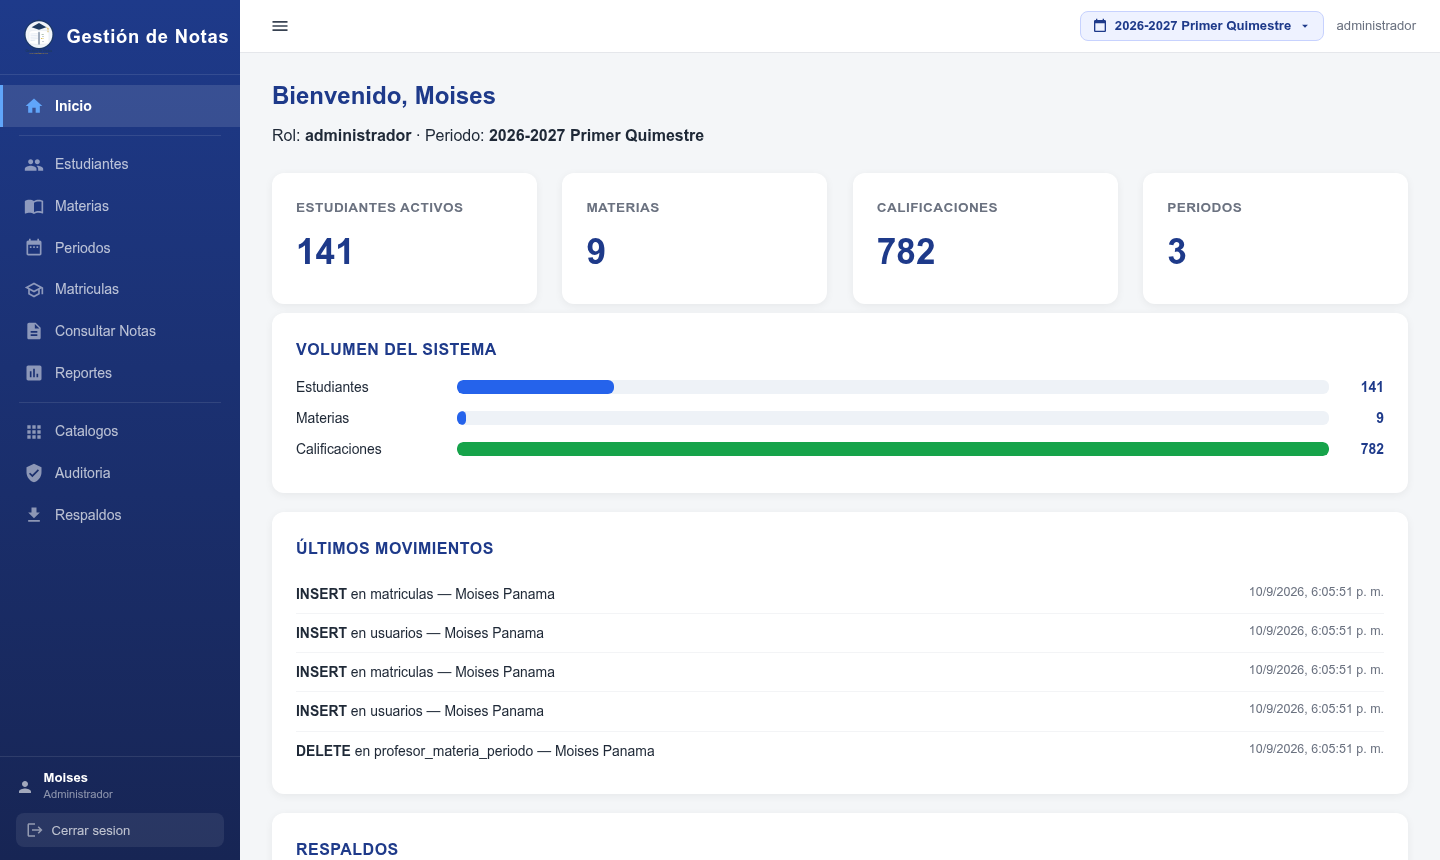
\includegraphics[width=0.92\textwidth]{evidencias/uat-01b_dashboard_admin.png}
\caption{Figura 15b. Dashboard del administrador: contadores, movimientos y respaldos recientes.}
\end{figure}


Interpretación: la redirección al dashboard y la sesión por cookie firmada funcionaron en los cinco perfiles; el control de acceso queda garantizado por el middleware de rol (403) y por la destrucción de sesión al cerrar (CP-14).


\subsubsection*{6.6.2 Gestión de estudiantes}
\addcontentsline{toc}{subsubsection}{6.6.2 Gestión de estudiantes}


El módulo de estudiantes valida el registro, la búsqueda por cédula/nombre y la unicidad de cédula. La captura muestra la planilla paginada con formato único \texttt{\{datos, paginacion\}} y los controles de filtrado.


\begin{figure}[H]
\centering
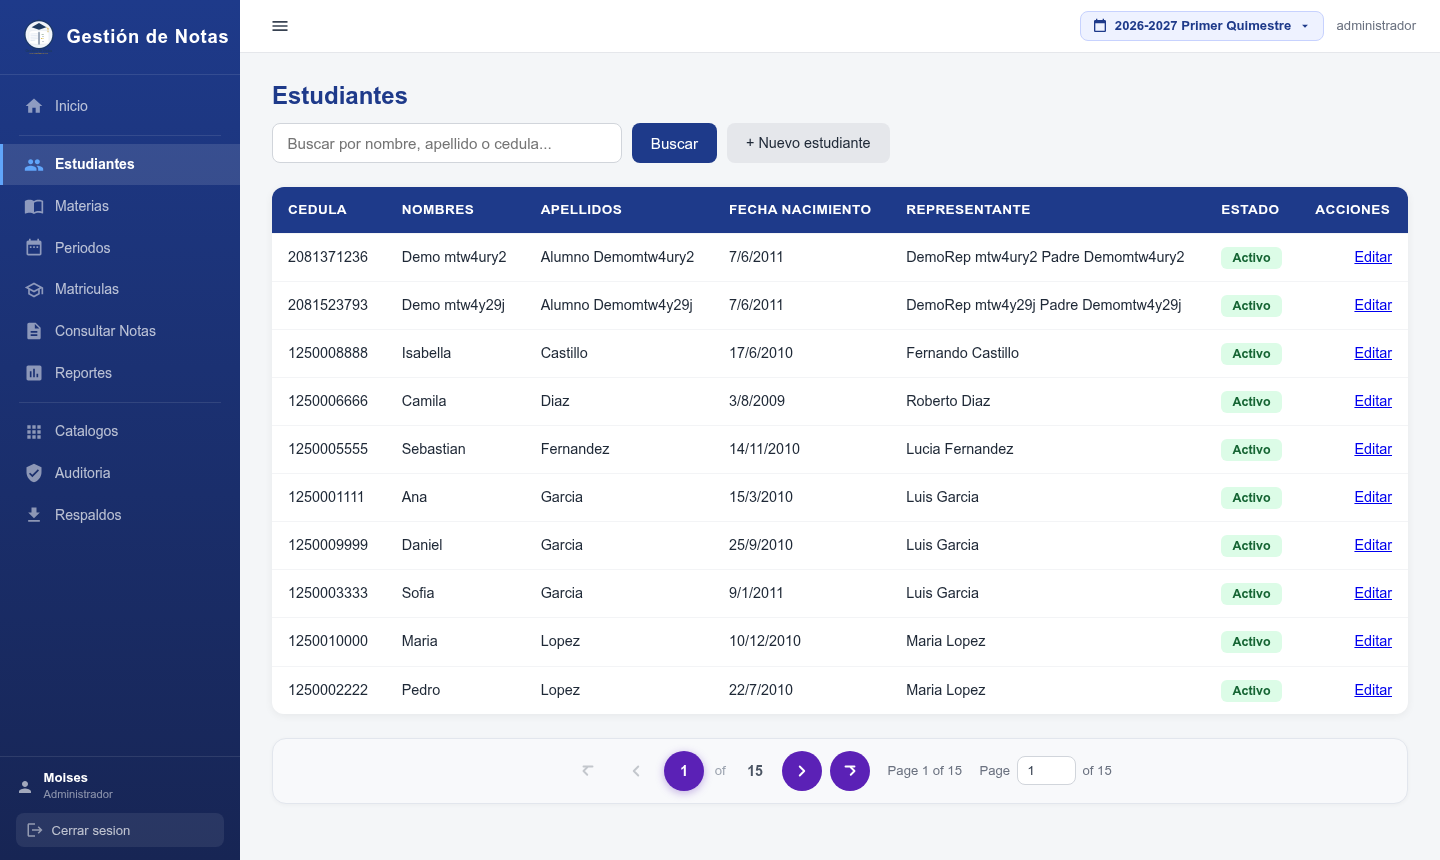
\includegraphics[width=0.92\textwidth]{evidencias/uat-02_estudiantes.png}
\caption{Figura 16. Planilla paginada de estudiantes con controles de búsqueda y paginación.}
\end{figure}


Interpretación: la paginación única (10 elementos por página) se corroboró también por API (estudiantes total=139, límite por defecto 10); la unicidad de cédula quedó protegida por el 409 (CP-03).


\subsubsection*{6.6.3 Registro de calificaciones (docente)}
\addcontentsline{toc}{subsubsection}{6.6.3 Registro de calificaciones (docente)}


El módulo del profesor muestra las materias asignadas en el periodo activo y la planilla de notas con ciclo y parcial. La captura del dashboard del docente y de la planilla de notas ilustra el flujo de captura masiva.


\begin{figure}[H]
\centering
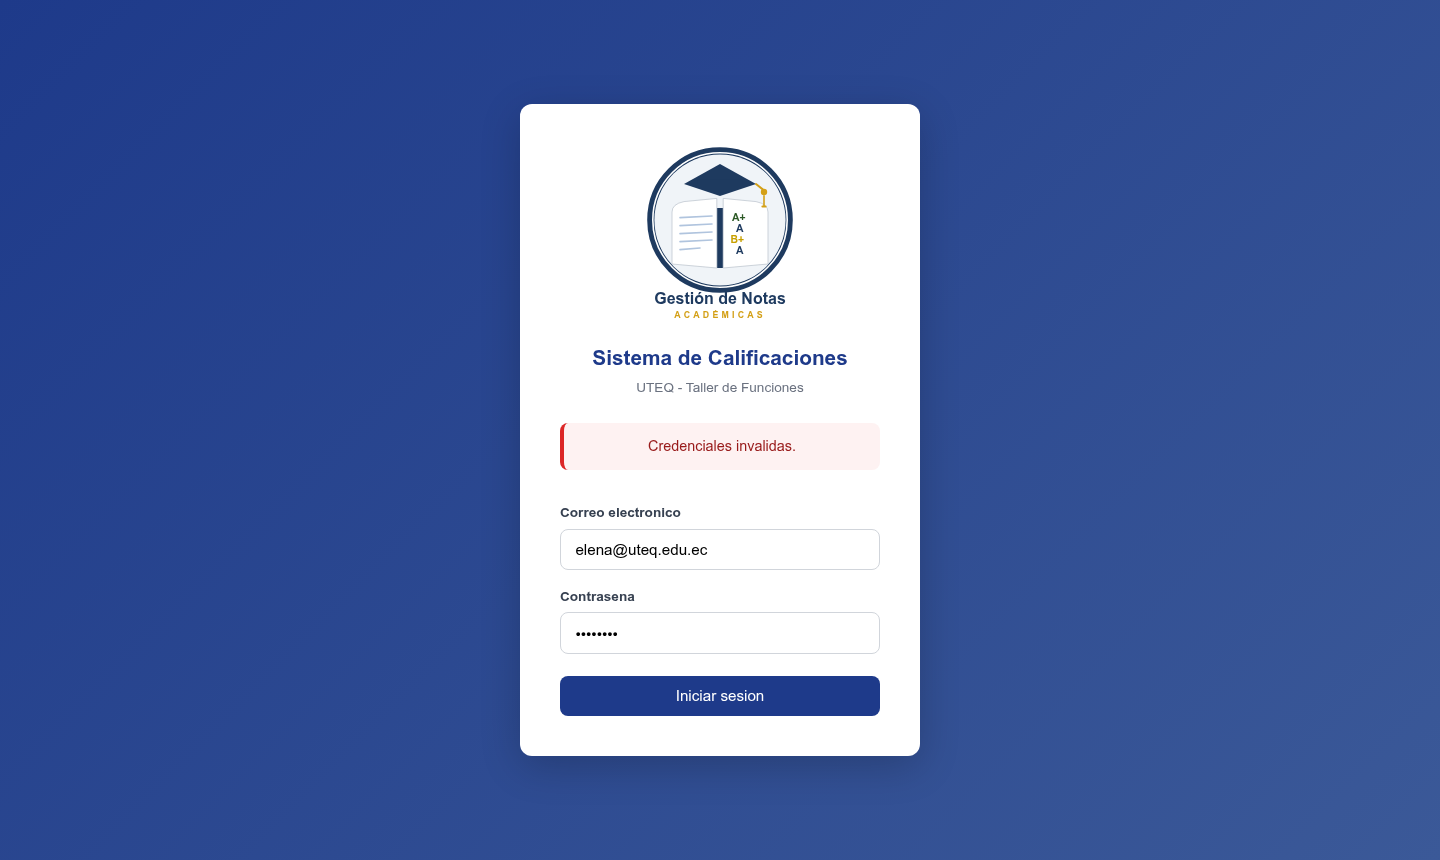
\includegraphics[width=0.92\textwidth]{evidencias/uat-03_dashboard_profesora.png}
\caption{Figura 17. Dashboard de la profesora con sus materias y últimas notas registradas.}
\end{figure}


\begin{figure}[H]
\centering
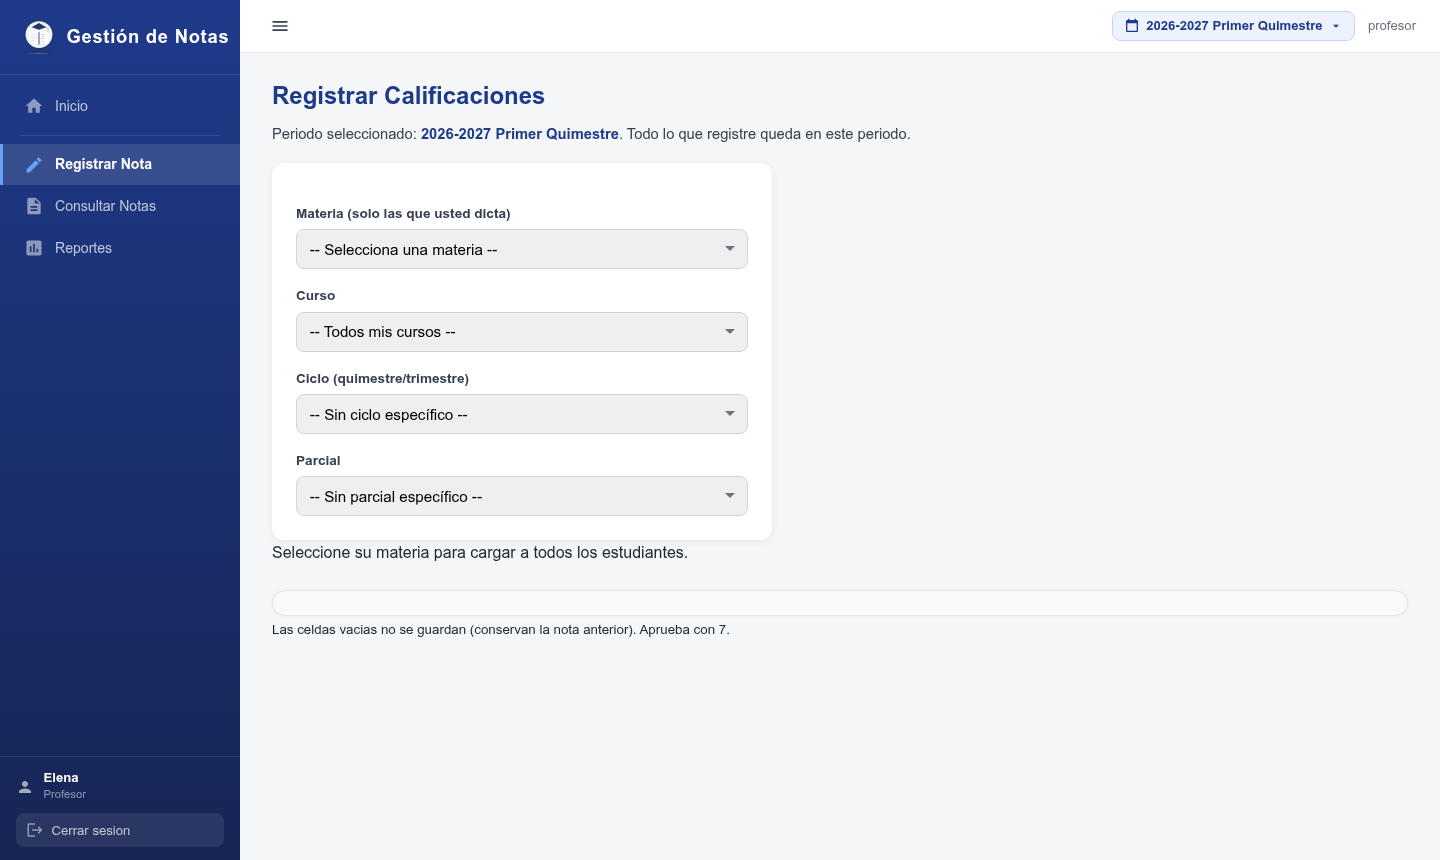
\includegraphics[width=0.92\textwidth]{evidencias/uat-03b_profesor_notas.png}
\caption{Figura 17b. Planilla de registro de calificaciones del profesor.}
\end{figure}


Interpretación: la validación de rango (0--10) y de materia asignada se confirmó por API (400/403) y por el trigger de base de datos; el guardado del lote se confirma con el mensaje ''Se guardaron N calificaciones.'' (CP-05).


\subsubsection*{6.6.4 Consulta del representante}
\addcontentsline{toc}{subsubsection}{6.6.4 Consulta del representante}


El representante ingresa y ve únicamente las notas de sus hijos, con promedio por materia, promedio general y escala cualitativa.


\begin{figure}[H]
\centering
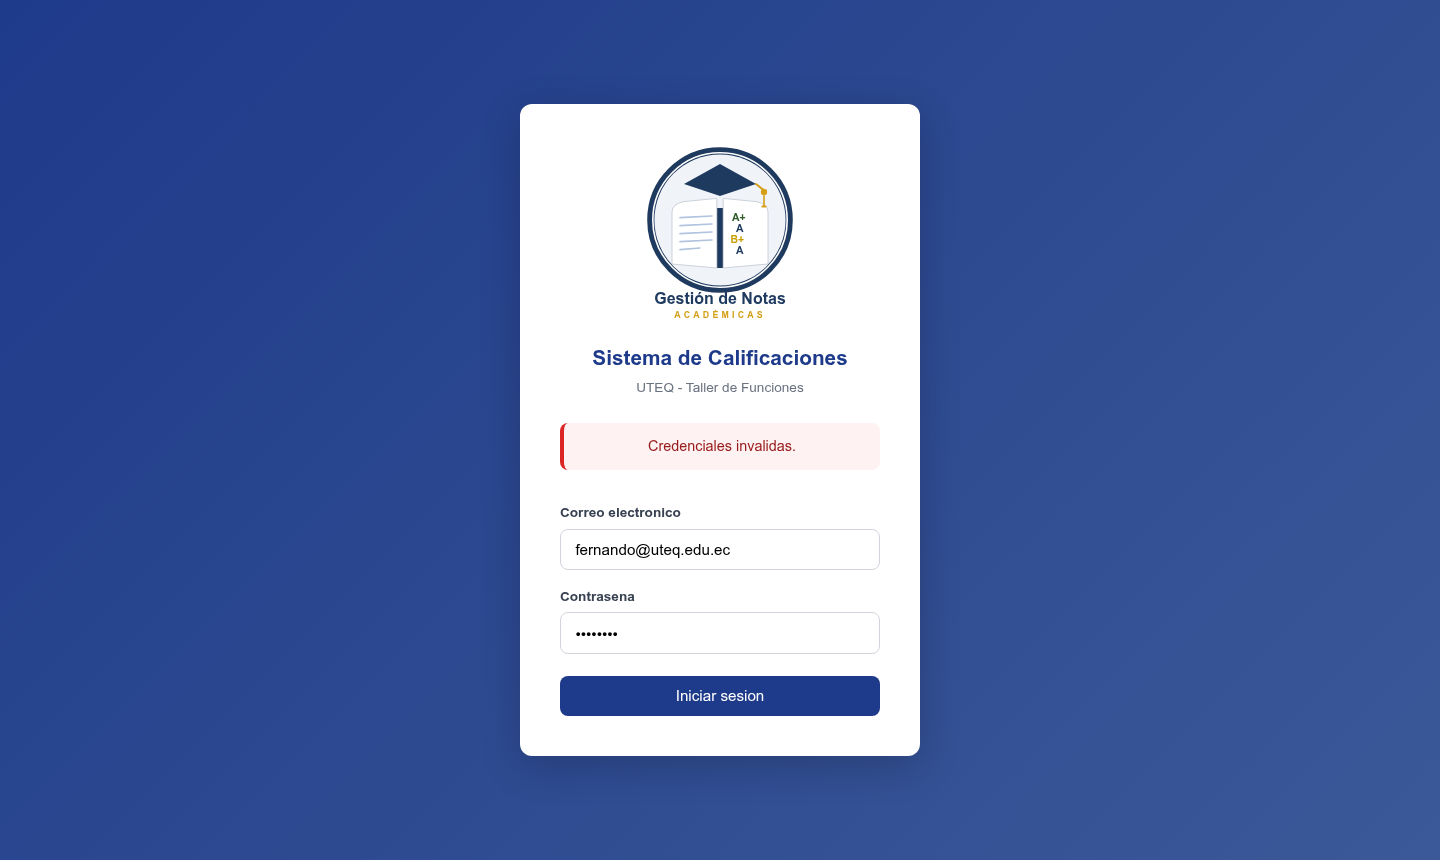
\includegraphics[width=0.92\textwidth]{evidencias/uat-04_representante.png}
\caption{Figura 18. Consulta de calificaciones del representante y desglose por materia.}
\end{figure}


\begin{figure}[H]
\centering
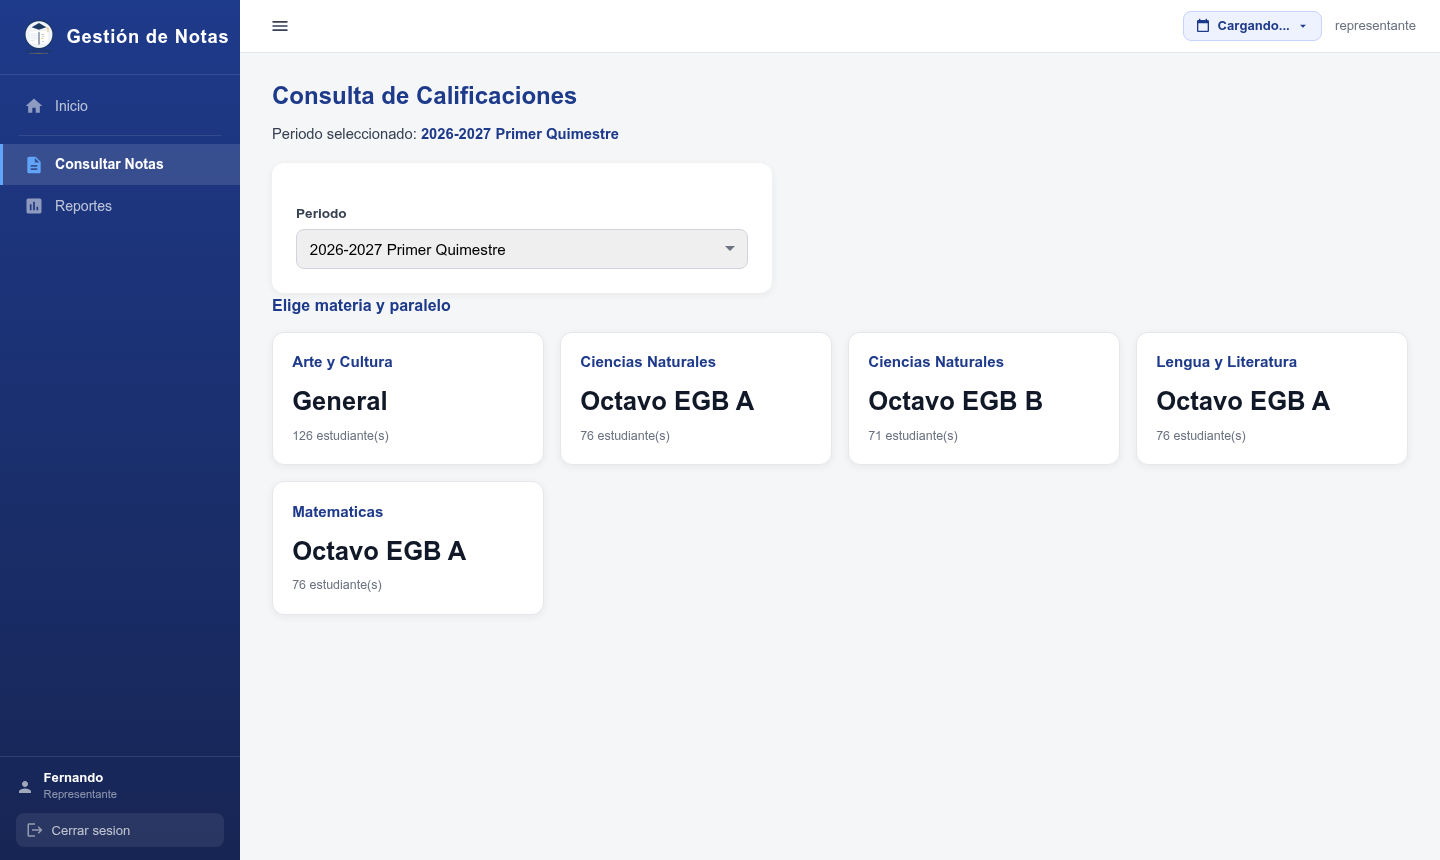
\includegraphics[width=0.92\textwidth]{evidencias/uat-04b_consulta_representante.png}
\caption{Figura 18b. Vista de la consulta del representante.}
\end{figure}


Interpretación: la restricción por rol (solo los hijos del representante) se verificó por UI y por API (dashboard de representante con 15 hijos y consulta forzada a lo propio en el rol estudiante).


\subsubsection*{6.6.5 Reportes de promedios}
\addcontentsline{toc}{subsubsection}{6.6.5 Reportes de promedios}


El módulo de reportes lista a los estudiantes ordenados por promedio descendente con su escala cualitativa.


\begin{figure}[H]
\centering
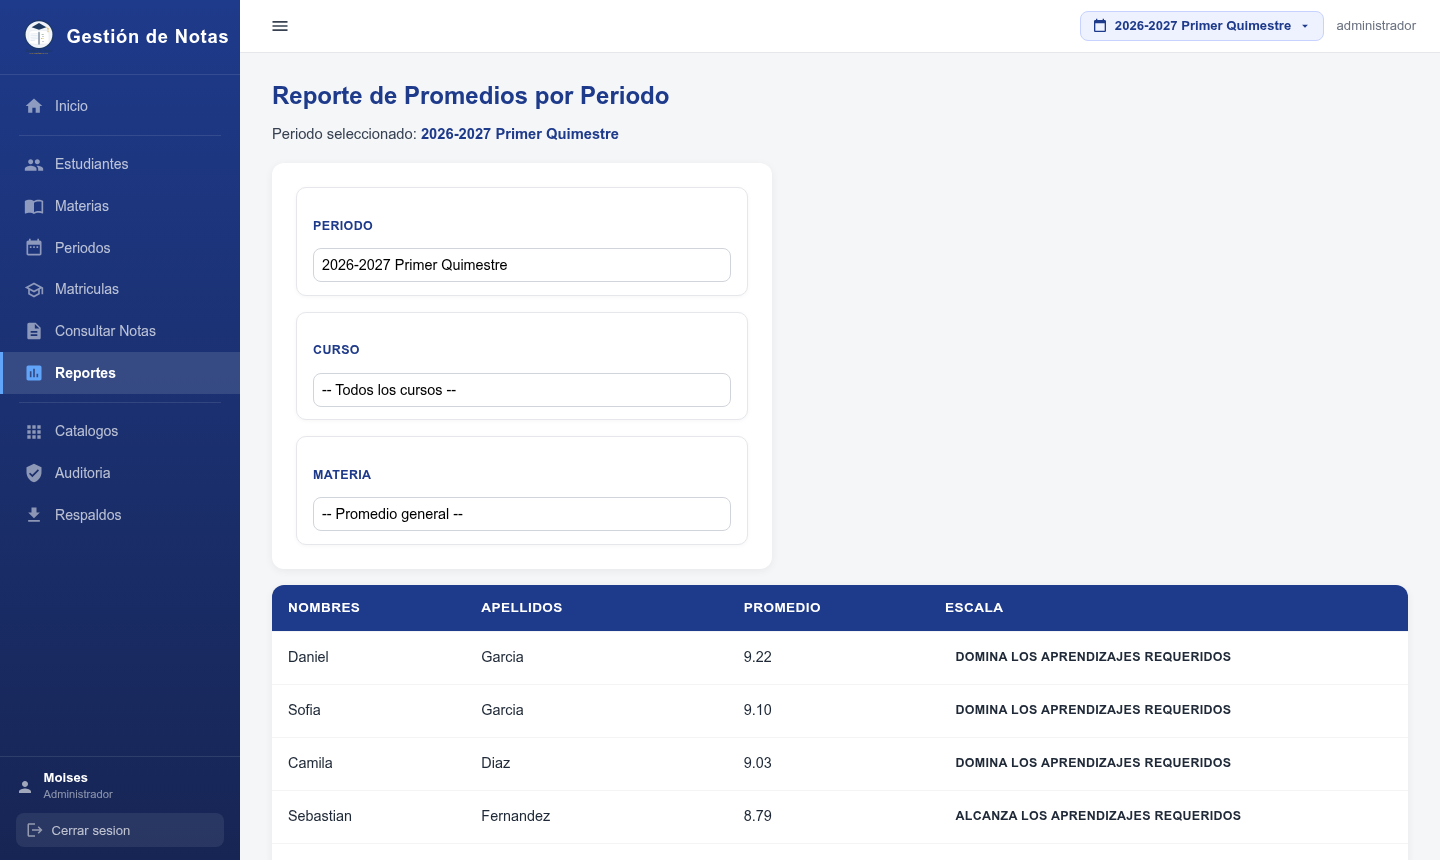
\includegraphics[width=0.92\textwidth]{evidencias/uat-05_reportes.png}
\caption{Figura 19. Reporte de promedios por periodo.}
\end{figure}


Interpretación: el cálculo coincide con la fórmula oficial (80\% parciales + 20\% examen); el filtro por curso incluye la opción ''Sin-curso'' (verificado por API con 50 filas) y la paginación se mantiene consistente.


\subsubsection*{6.6.6 Auditoría}
\addcontentsline{toc}{subsubsection}{6.6.6 Auditoría}


El panel de auditoría permite al administrador revisar el historial con datos antes/después en JSONB y el usuario de la aplicación; los no administradores reciben 403.


\begin{figure}[H]
\centering
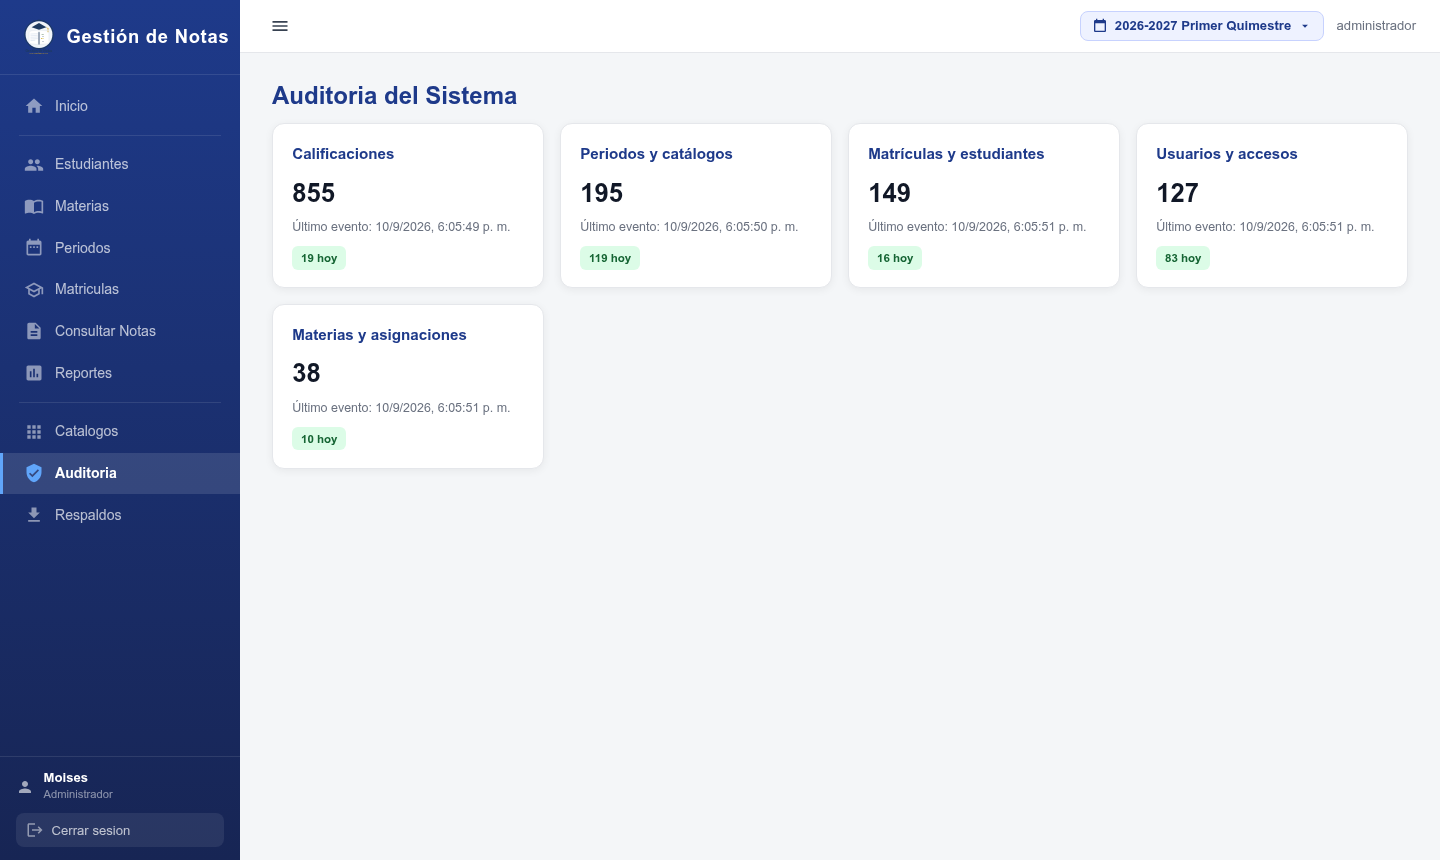
\includegraphics[width=0.92\textwidth]{evidencias/uat-06_auditoria.png}
\caption{Figura 20. Panel de auditoría del administrador.}
\end{figure}


Interpretación: la auditoría acumula registros por cada operación de negocio; en la corrida documentada el total fue de 855 registros (API) y el panel los presenta con filtros por fecha y categoría y con resumen por bloques.


\subsubsection*{6.6.7 Rendimiento de la psicóloga}
\addcontentsline{toc}{subsubsection}{6.6.7 Rendimiento de la psicóloga}


El panel de psicóloga presenta el resumen de rendimiento (total, alertas, promedios) y el detalle por estudiante con un máximo de 10 filas.


\begin{figure}[H]
\centering
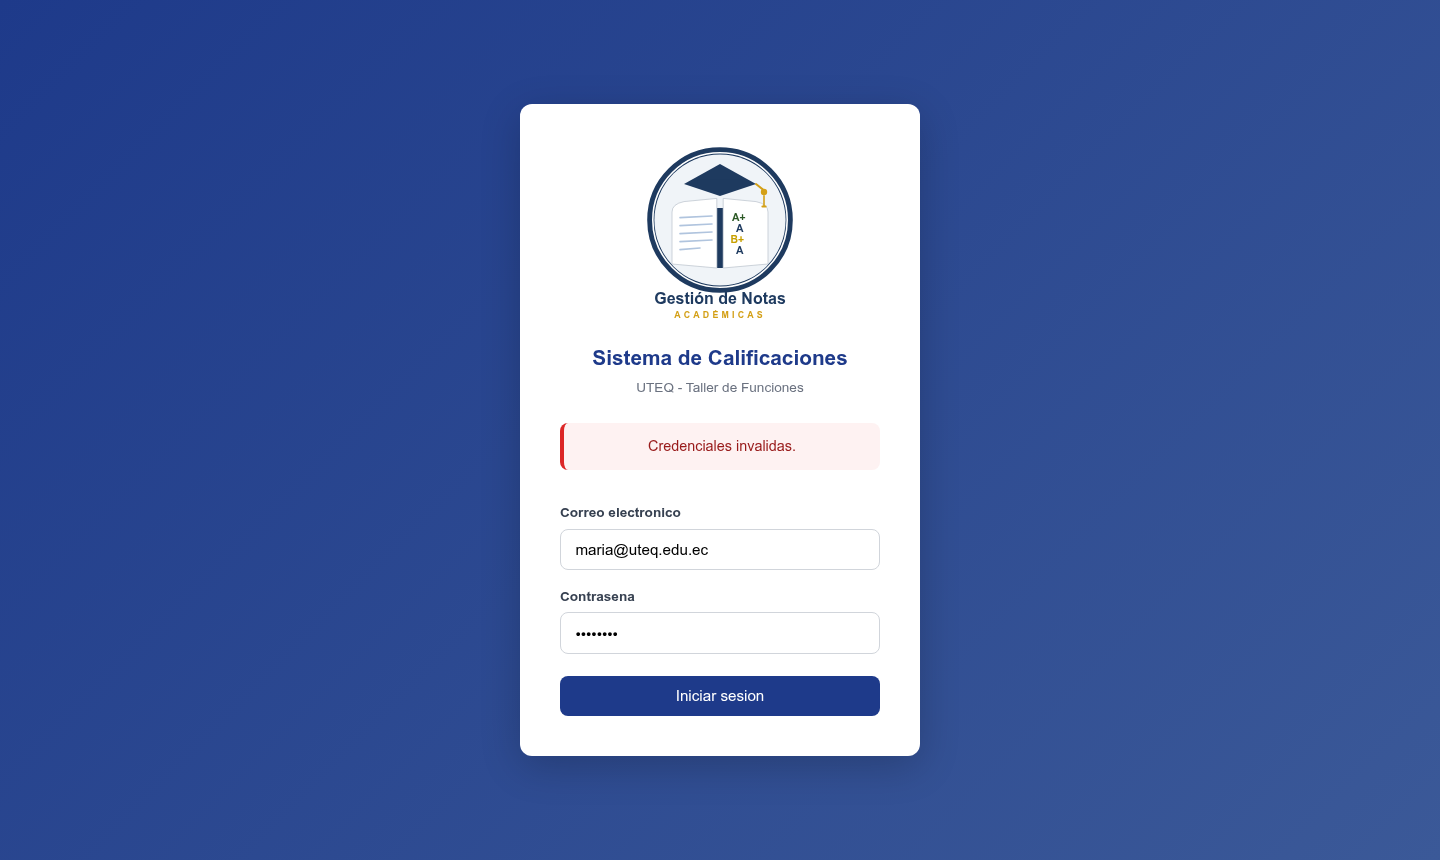
\includegraphics[width=0.92\textwidth]{evidencias/uat-07_psicologa.png}
\caption{Figura 21. Dashboard de la psicóloga.}
\end{figure}


\begin{figure}[H]
\centering
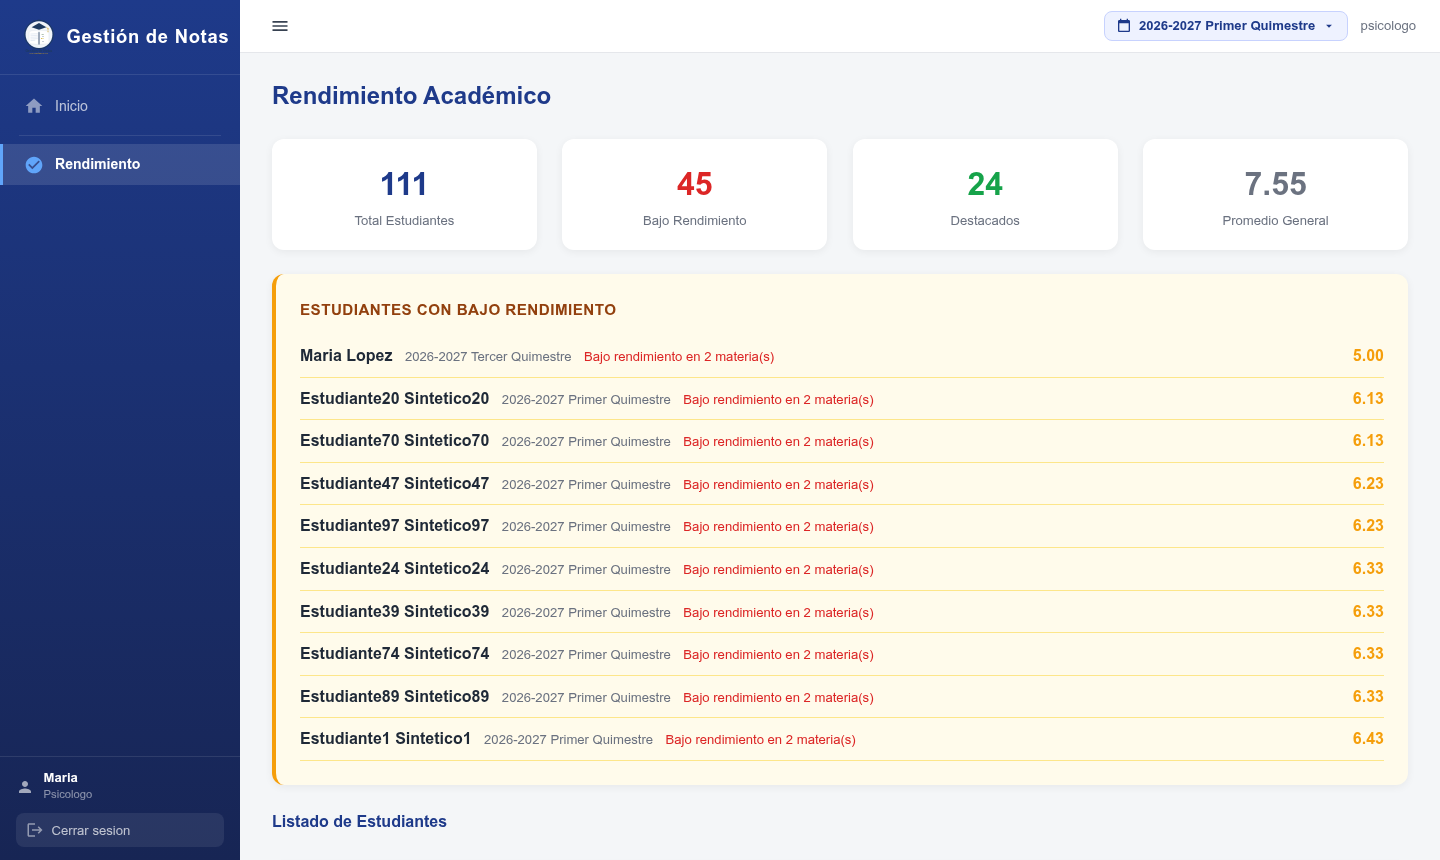
\includegraphics[width=0.92\textwidth]{evidencias/uat-07b_psicologa_panel.png}
\caption{Figura 21b. Panel de rendimiento académico con alertas.}
\end{figure}


Interpretación: el resumen devuelto por \texttt{/psicologo/rendimiento} (total=111, alertas=10 en la corrida de la API) se refleja correctamente en la interfaz, y el acceso de un administrador al módulo se bloquea con 403 (test 35 de la suite UI).


\subsubsection*{6.6.8 Rol estudiante}
\addcontentsline{toc}{subsubsection}{6.6.8 Rol estudiante}


El rol estudiante (incorporado en la migración 21) permite al alumno consultar únicamente sus propias notas: sin accesos a reportes, sin nóminas de otras personas y sin botones de regreso a bloques/nómina. Los 5 tests de \texttt{estudiante.spec.cjs} y los checks 13--14 de la suite API lo confirmaron (consulta ajena devuelve lo propio; \texttt{/reportes} responde 403).


\hrule\vspace{0.4em}


\section*{7. Casos de prueba de aceptación del usuario (UAT)}
\addcontentsline{toc}{section}{7. Casos de prueba de aceptación del usuario (UAT)}


\subsection*{7.1 Enfoque}
\addcontentsline{toc}{subsection}{7.1 Enfoque}


Los casos UAT validan que el sistema cumple \textbf{el criterio de aceptación del usuario final}, no solo la implementación técnica. Se definieron 7 casos (uno por historia principal) ejecutados con los perfiles de la técnica Personas (administrador, profesor, representante y psicóloga). Cada caso referencia su historia de usuario (HU) y sus criterios de aceptación (CA).


\subsection*{7.2 UAT-01 --- ''Puedo entrar a mi cuenta de administrador''}
\addcontentsline{toc}{subsection}{7.2 UAT-01 --- ''Puedo entrar a mi cuenta de administrador''}


{\small
\begin{longtable}{|p{\dimexpr\textwidth/2-2\tabcolsep\relax}|p{\dimexpr\textwidth/2-2\tabcolsep\relax}|}
\rowcolor{UTECblue}\color{white}\bfseries Atributo & \color{white}\bfseries Detalle \\ \hline
\endfirsthead
\rowcolor{UTECblue}\color{white}\bfseries Atributo & \color{white}\bfseries Detalle \\ \hline
\endhead
Historia / Criterio & HU-01 / CA-1 \\ \hline
Rol & Administrador (Moisés) \\ \hline
Pasos & Abrir el sistema {$\rightarrow$} ingresar correo y contraseña {$\rightarrow$} confirmar acceso \\ \hline
Datos & \texttt{admin@uteq.edu.ec} / \texttt{UTEQ2026} \\ \hline
Resultado esperado & Veo mi panel de administración con mi nombre \\ \hline
Resultado obtenido & Acceso correcto al dashboard, nombre y rol visibles \\ \hline
Aceptación & {\color{green!60!black}{$\checkmark$}} \textbf{ACEPTADO} \\ \hline
Evidencia & \texttt{evidencias/uat-01\_login\_admin.png} \\ \hline
\end{longtable}}


\begin{figure}[H]
\centering

\includegraphics[width=0.92\textwidth]{evidencias/uat-01_login_admin.png}
\caption{Figura 22. Formulario de inicio de sesión del caso UAT-01.}
\end{figure}


\subsection*{7.3 UAT-02 --- ''Puedo registrar y buscar estudiantes''}
\addcontentsline{toc}{subsection}{7.3 UAT-02 --- ''Puedo registrar y buscar estudiantes''}


{\small
\begin{longtable}{|p{\dimexpr\textwidth/2-2\tabcolsep\relax}|p{\dimexpr\textwidth/2-2\tabcolsep\relax}|}
\rowcolor{UTECblue}\color{white}\bfseries Atributo & \color{white}\bfseries Detalle \\ \hline
\endfirsthead
\rowcolor{UTECblue}\color{white}\bfseries Atributo & \color{white}\bfseries Detalle \\ \hline
\endhead
Historia / Criterio & HU-02 / CA-1, CA-2 \\ \hline
Rol & Administrador \\ \hline
Pasos & Abrir Estudiantes {$\rightarrow$} registrar un nuevo estudiante {$\rightarrow$} buscarlo por cédula \\ \hline
Datos & Estudiante de prueba UAT-02; cédula única \\ \hline
Resultado esperado & El estudiante aparece en la lista y es localizable por cédula \\ \hline
Resultado obtenido & Registro exitoso y búsqueda devuelve la fila correcta \\ \hline
Aceptación & {\color{green!60!black}{$\checkmark$}} \textbf{ACEPTADO} \\ \hline
Evidencia & \texttt{evidencias/uat-02\_estudiantes.png} \\ \hline
\end{longtable}}


\begin{figure}[H]
\centering
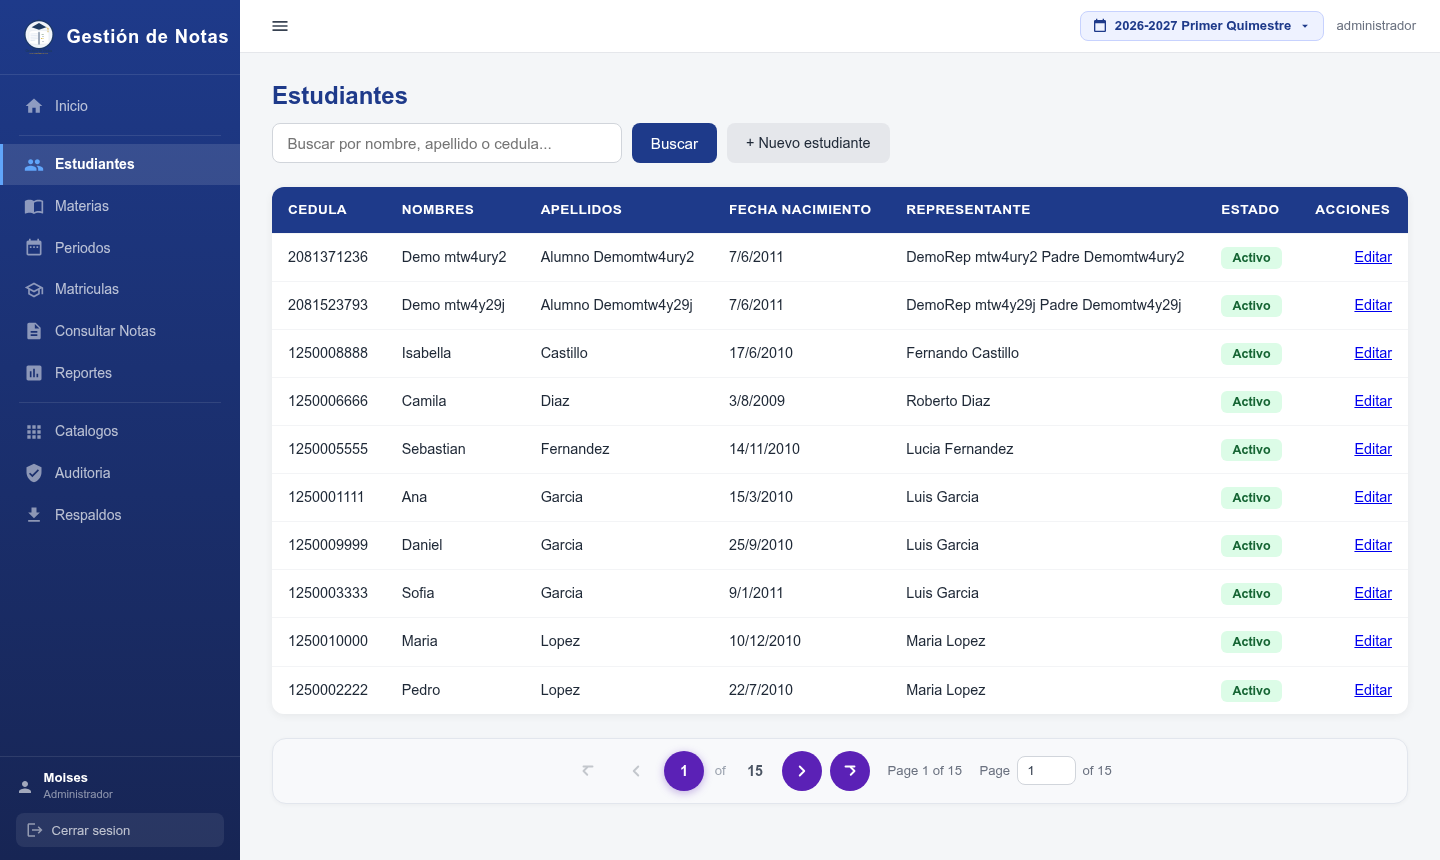
\includegraphics[width=0.92\textwidth]{evidencias/uat-02_estudiantes.png}
\caption{Figura 23. Planilla de estudiantes del caso UAT-02.}
\end{figure}


\subsection*{7.4 UAT-03 --- ''Puedo registrar las notas de mi materia fácilmente''}
\addcontentsline{toc}{subsection}{7.4 UAT-03 --- ''Puedo registrar las notas de mi materia fácilmente''}


{\small
\begin{longtable}{|p{\dimexpr\textwidth/2-2\tabcolsep\relax}|p{\dimexpr\textwidth/2-2\tabcolsep\relax}|}
\rowcolor{UTECblue}\color{white}\bfseries Atributo & \color{white}\bfseries Detalle \\ \hline
\endfirsthead
\rowcolor{UTECblue}\color{white}\bfseries Atributo & \color{white}\bfseries Detalle \\ \hline
\endhead
Historia / Criterio & HU-03 / CA-1 a CA-4 \\ \hline
Rol & Profesora (Elena) \\ \hline
Pasos & Abrir Calificaciones {$\rightarrow$} elegir mi materia {$\rightarrow$} digitar notas 0--10 {$\rightarrow$} guardar todo \\ \hline
Datos & Materia: Ciencias Naturales; notas parciales válidas \\ \hline
Resultado esperado & Todas las notas se guardan a la vez y veo confirmación \\ \hline
Resultado obtenido & ''Se guardaron N calificaciones.'' y las notas se reflejan en la consulta \\ \hline
Aceptación & {\color{green!60!black}{$\checkmark$}} \textbf{ACEPTADO} \\ \hline
Evidencia & \texttt{evidencias/uat-03b\_profesor\_notas.png} \\ \hline
\end{longtable}}


\begin{figure}[H]
\centering
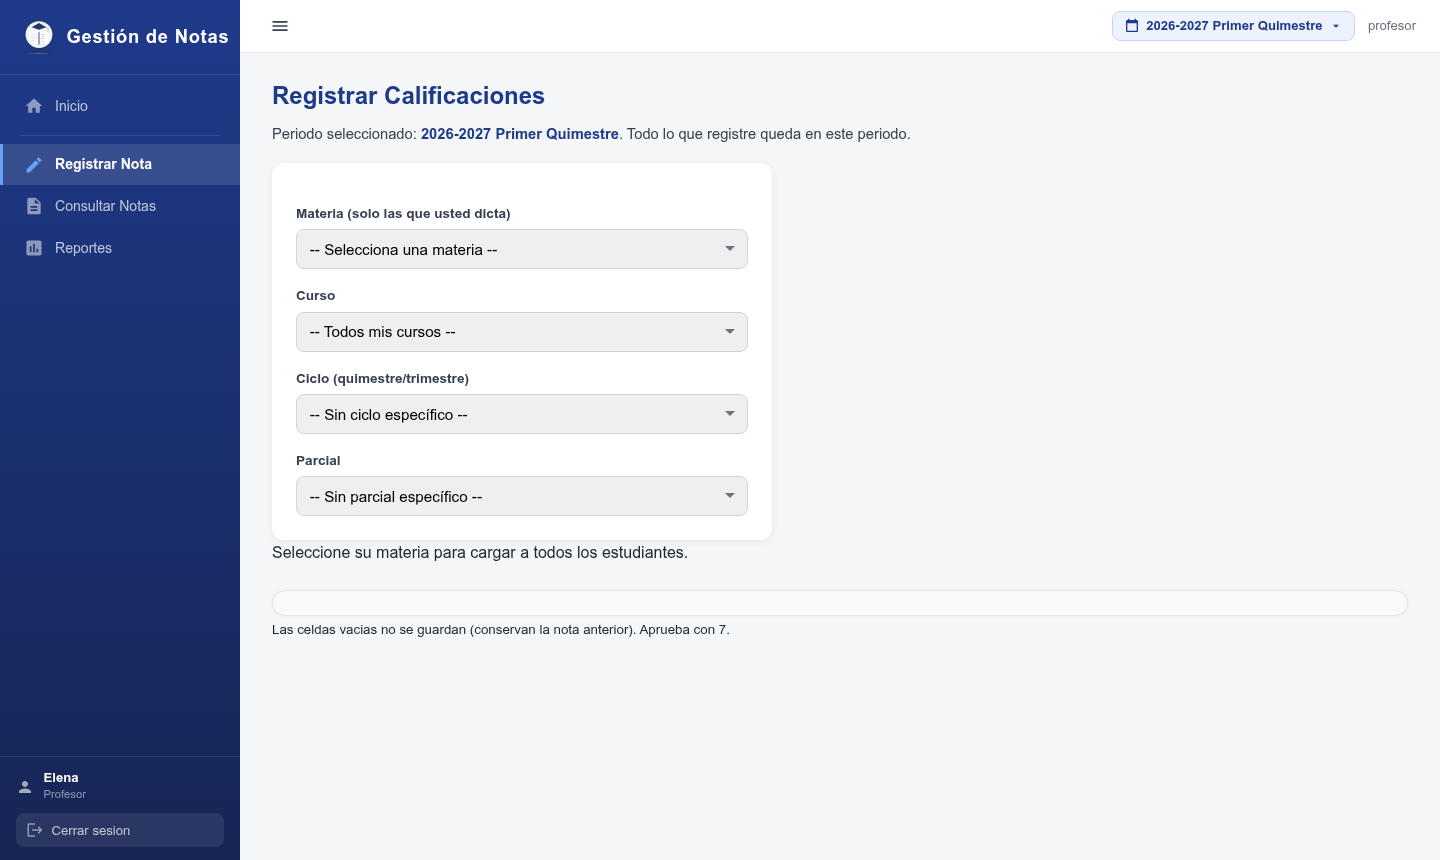
\includegraphics[width=0.92\textwidth]{evidencias/uat-03b_profesor_notas.png}
\caption{Figura 24. Planilla de notas del profesor (UAT-03).}
\end{figure}


\subsection*{7.5 UAT-04 --- ''Veo las notas de mi hijo sin ver las de otros''}
\addcontentsline{toc}{subsection}{7.5 UAT-04 --- ''Veo las notas de mi hijo sin ver las de otros''}


{\small
\begin{longtable}{|p{\dimexpr\textwidth/2-2\tabcolsep\relax}|p{\dimexpr\textwidth/2-2\tabcolsep\relax}|}
\rowcolor{UTECblue}\color{white}\bfseries Atributo & \color{white}\bfseries Detalle \\ \hline
\endfirsthead
\rowcolor{UTECblue}\color{white}\bfseries Atributo & \color{white}\bfseries Detalle \\ \hline
\endhead
Historia / Criterio & HU-04 / CA-1, CA-2 \\ \hline
Rol & Representante (Fernando) \\ \hline
Pasos & Ingresar {$\rightarrow$} elegir a mi hijo {$\rightarrow$} revisar notas y promedio \\ \hline
Datos & Hijo: Isabella Castillo \\ \hline
Resultado esperado & Solo veo las notas de mis hijos, con promedio y escala \\ \hline
Resultado obtenido & Consulta restringida correctamente a los hijos del representante \\ \hline
Aceptación & {\color{green!60!black}{$\checkmark$}} \textbf{ACEPTADO} \\ \hline
Evidencia & \texttt{evidencias/uat-04b\_consulta\_representante.png} \\ \hline
\end{longtable}}


\begin{figure}[H]
\centering
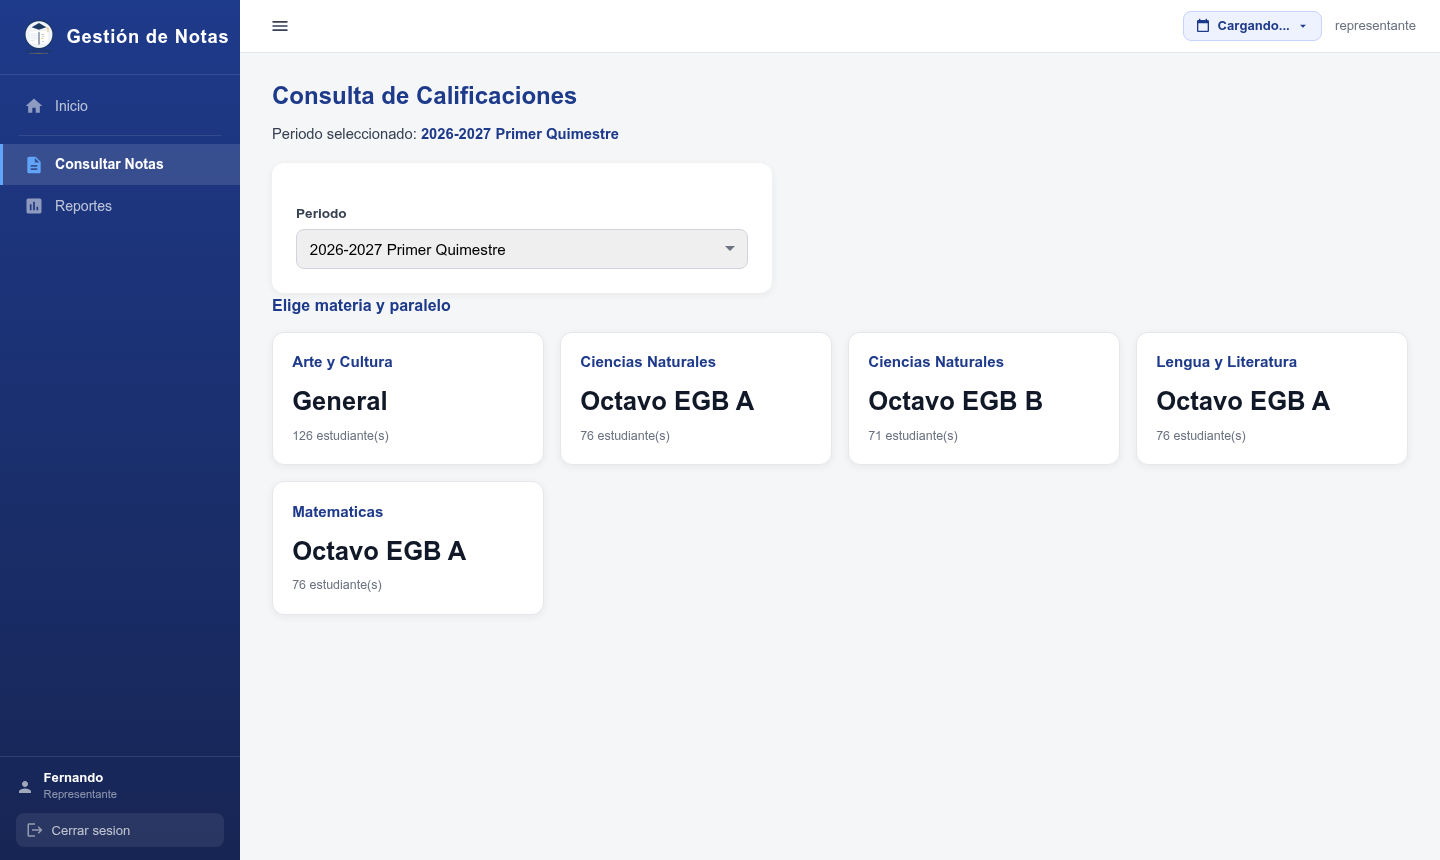
\includegraphics[width=0.92\textwidth]{evidencias/uat-04b_consulta_representante.png}
\caption{Figura 25. Consulta del representante (UAT-04).}
\end{figure}


\subsection*{7.6 UAT-05 --- ''Veo el reporte de promedios del periodo''}
\addcontentsline{toc}{subsection}{7.6 UAT-05 --- ''Veo el reporte de promedios del periodo''}


{\small
\begin{longtable}{|p{\dimexpr\textwidth/2-2\tabcolsep\relax}|p{\dimexpr\textwidth/2-2\tabcolsep\relax}|}
\rowcolor{UTECblue}\color{white}\bfseries Atributo & \color{white}\bfseries Detalle \\ \hline
\endfirsthead
\rowcolor{UTECblue}\color{white}\bfseries Atributo & \color{white}\bfseries Detalle \\ \hline
\endhead
Historia / Criterio & HU-05 / CA-1 a CA-3 \\ \hline
Rol & Administrador \\ \hline
Pasos & Abrir Reportes {$\rightarrow$} seleccionar periodo y consultar \\ \hline
Datos & Periodo activo (2026-2027 Primer Quimestre) \\ \hline
Resultado esperado & Listado ordenado por promedio con escala cualitativa \\ \hline
Resultado obtenido & 10 estudiantes ordenados de mayor a menor promedio \\ \hline
Aceptación & {\color{green!60!black}{$\checkmark$}} \textbf{ACEPTADO} \\ \hline
Evidencia & \texttt{evidencias/uat-05\_reportes.png} \\ \hline
\end{longtable}}


\begin{figure}[H]
\centering
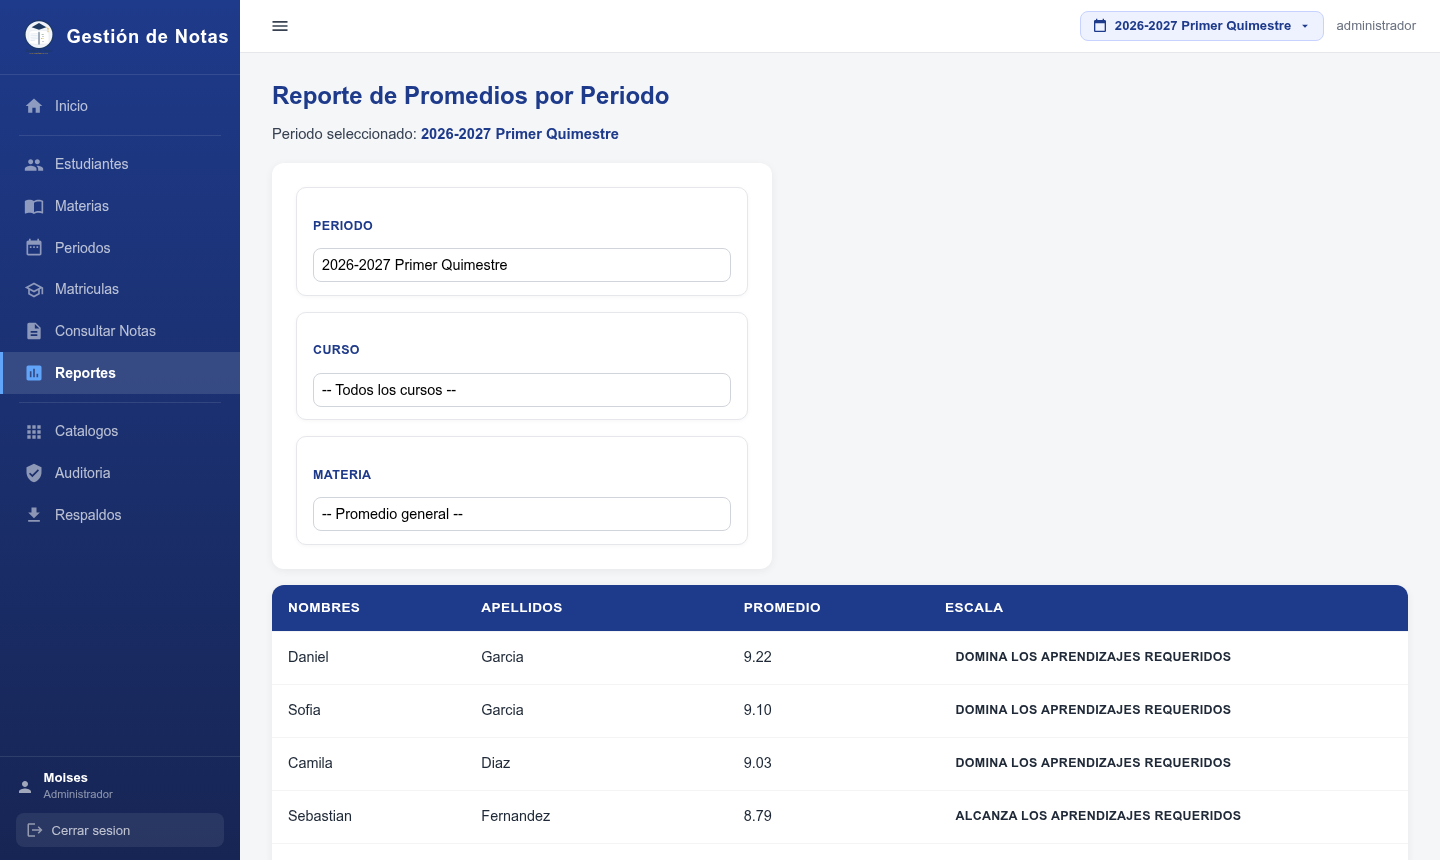
\includegraphics[width=0.92\textwidth]{evidencias/uat-05_reportes.png}
\caption{Figura 26. Reporte de promedios (UAT-05).}
\end{figure}


\subsection*{7.7 UAT-06 --- ''Puedo auditar qué cambió y quién lo hizo''}
\addcontentsline{toc}{subsection}{7.7 UAT-06 --- ''Puedo auditar qué cambió y quién lo hizo''}


{\small
\begin{longtable}{|p{\dimexpr\textwidth/2-2\tabcolsep\relax}|p{\dimexpr\textwidth/2-2\tabcolsep\relax}|}
\rowcolor{UTECblue}\color{white}\bfseries Atributo & \color{white}\bfseries Detalle \\ \hline
\endfirsthead
\rowcolor{UTECblue}\color{white}\bfseries Atributo & \color{white}\bfseries Detalle \\ \hline
\endhead
Historia / Criterio & HU-06 / CA-1 a CA-4 \\ \hline
Rol & Administrador \\ \hline
Pasos & Abrir Auditoría {$\rightarrow$} revisar operaciones {$\rightarrow$} confirmar que un rol no administrador NO puede verla \\ \hline
Datos & Registros generados previamente (p. ej., notas de Elena) \\ \hline
Resultado esperado & Veo la tabla de auditoría con datos antes/después y el usuario que operó \\ \hline
Resultado obtenido & Panel con registros JSONB y usuario de la aplicación; bloqueo a no-admin verificado \\ \hline
Aceptación & {\color{green!60!black}{$\checkmark$}} \textbf{ACEPTADO} \\ \hline
Evidencia & \texttt{evidencias/playwright-03-admin-auditoria.png} {$\cdot$} \texttt{e2e\_test\_repo\_66.txt} \\ \hline
\end{longtable}}


\begin{figure}[H]
\centering
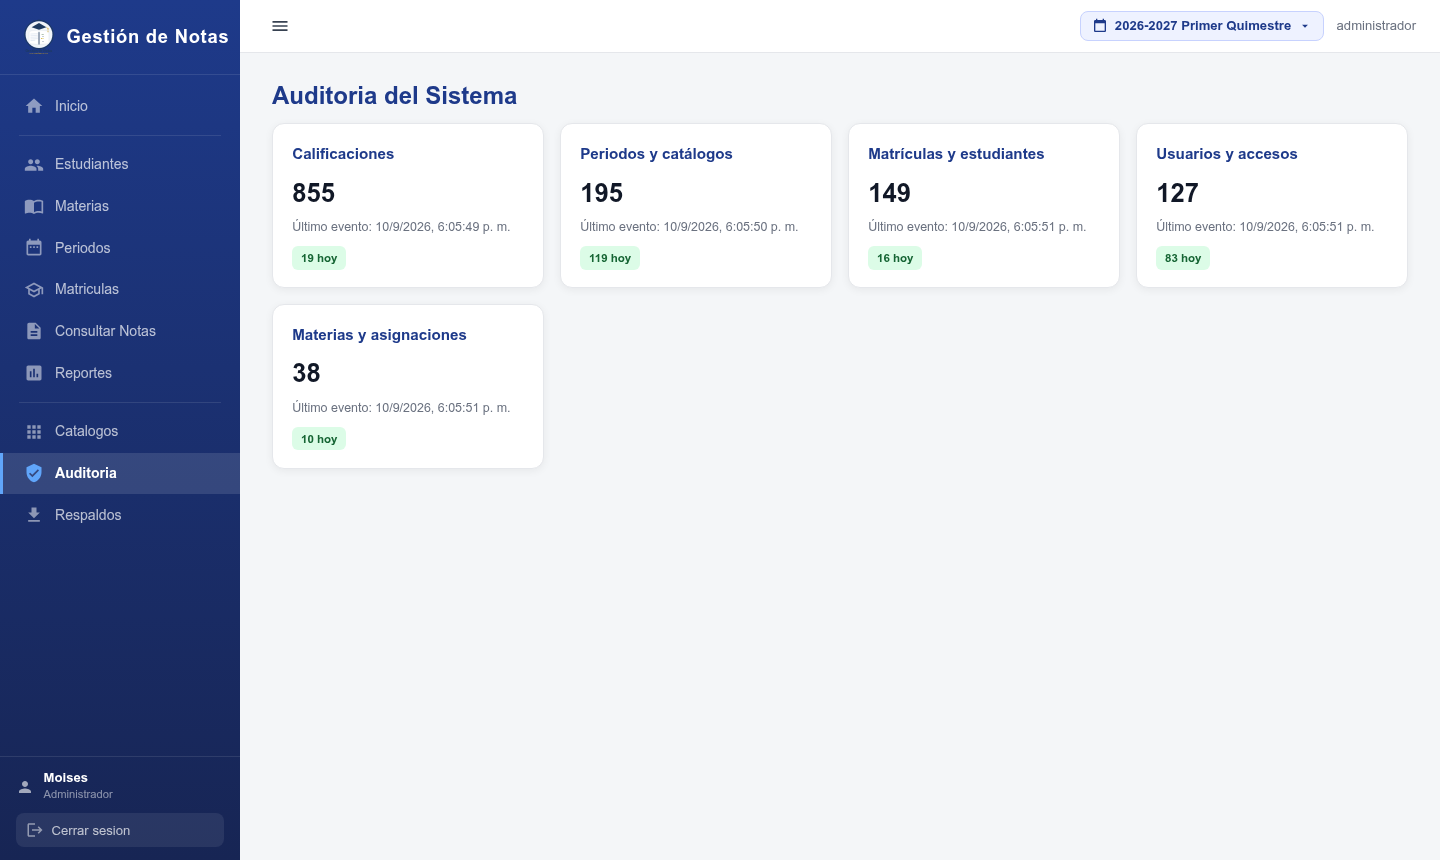
\includegraphics[width=0.92\textwidth]{evidencias/uat-06_auditoria.png}
\caption{Figura 27. Panel de auditoría (UAT-06).}
\end{figure}


\subsection*{7.8 UAT-07 --- ''La psicóloga ve el rendimiento de los estudiantes para dar acompañamiento''}
\addcontentsline{toc}{subsection}{7.8 UAT-07 --- ''La psicóloga ve el rendimiento de los estudiantes para dar acompañamiento''}


{\small
\begin{longtable}{|p{\dimexpr\textwidth/2-2\tabcolsep\relax}|p{\dimexpr\textwidth/2-2\tabcolsep\relax}|}
\rowcolor{UTECblue}\color{white}\bfseries Atributo & \color{white}\bfseries Detalle \\ \hline
\endfirsthead
\rowcolor{UTECblue}\color{white}\bfseries Atributo & \color{white}\bfseries Detalle \\ \hline
\endhead
Historia / Criterio & HU-09 / CA-1 a CA-3 \\ \hline
Rol & Psicóloga (María) \\ \hline
Pasos & Abrir el panel de psicóloga {$\rightarrow$} revisar el resumen {$\rightarrow$} abrir el detalle de un estudiante \\ \hline
Datos & Periodo activo \\ \hline
Resultado esperado & Resumen de rendimiento, listado de estudiantes y detalle por materia \\ \hline
Resultado obtenido & Resumen con total y alertas, y detalle por estudiante \\ \hline
Aceptación & {\color{green!60!black}{$\checkmark$}} \textbf{ACEPTADO} \\ \hline
Evidencia & \texttt{evidencias/uat-07b\_psicologa\_panel.png} \\ \hline
\end{longtable}}


\begin{figure}[H]
\centering
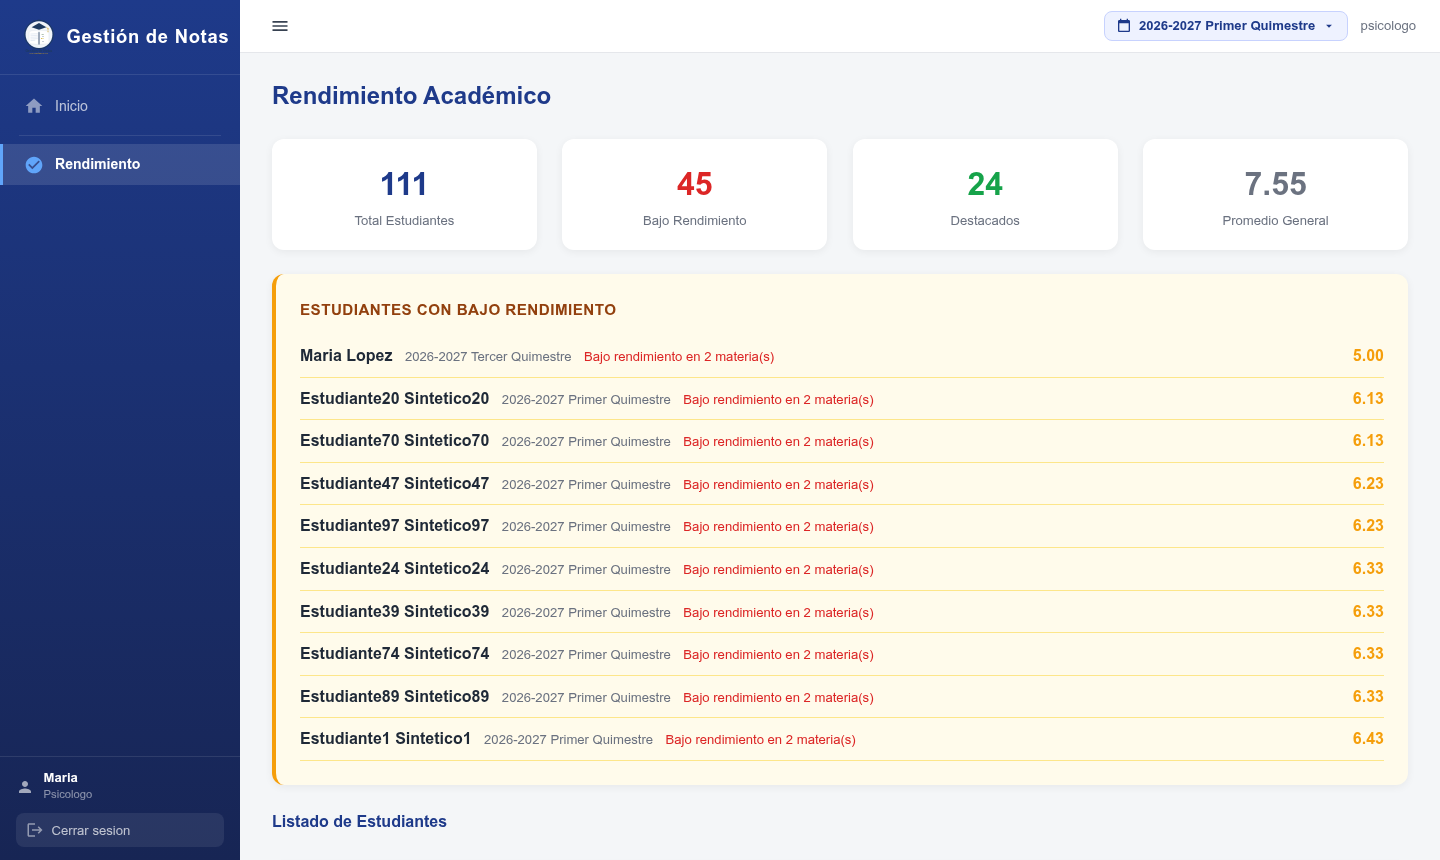
\includegraphics[width=0.92\textwidth]{evidencias/uat-07b_psicologa_panel.png}
\caption{Figura 28. Panel de rendimiento de la psicóloga (UAT-07).}
\end{figure}


\subsection*{7.9 Resumen UAT}
\addcontentsline{toc}{subsection}{7.9 Resumen UAT}


\textbf{Tabla 9. Resumen de casos UAT.}


{\small
\begin{longtable}{|p{\dimexpr\textwidth/4-2\tabcolsep\relax}|p{\dimexpr\textwidth/4-2\tabcolsep\relax}|p{\dimexpr\textwidth/4-2\tabcolsep\relax}|p{\dimexpr\textwidth/4-2\tabcolsep\relax}|}
\rowcolor{UTECblue}\color{white}\bfseries \# & \color{white}\bfseries Historia & \color{white}\bfseries Resultado & \color{white}\bfseries Decisión \\ \hline
\endfirsthead
\rowcolor{UTECblue}\color{white}\bfseries \# & \color{white}\bfseries Historia & \color{white}\bfseries Resultado & \color{white}\bfseries Decisión \\ \hline
\endhead
UAT-01 & HU-01 & {\color{green!60!black}{$\checkmark$}} PASS & ACEPTADO \\ \hline
UAT-02 & HU-02 & {\color{green!60!black}{$\checkmark$}} PASS & ACEPTADO \\ \hline
UAT-03 & HU-03 & {\color{green!60!black}{$\checkmark$}} PASS & ACEPTADO \\ \hline
UAT-04 & HU-04 & {\color{green!60!black}{$\checkmark$}} PASS & ACEPTADO \\ \hline
UAT-05 & HU-05 & {\color{green!60!black}{$\checkmark$}} PASS & ACEPTADO \\ \hline
UAT-06 & HU-06 & {\color{green!60!black}{$\checkmark$}} PASS & ACEPTADO \\ \hline
UAT-07 & HU-09 & {\color{green!60!black}{$\checkmark$}} PASS & ACEPTADO \\ \hline
\end{longtable}}


\textbf{Conclusión UAT:} el 100\% de los criterios de aceptación definidos por el usuario fueron cumplidos. El sistema queda \textbf{aprobado para producción} por el usuario final.


\hrule\vspace{0.4em}


\section*{8. Prueba de la versión Beta}
\addcontentsline{toc}{section}{8. Prueba de la versión Beta}


\subsection*{8.1 Objetivo}
\addcontentsline{toc}{subsection}{8.1 Objetivo}


Validar el sistema en condiciones reales de uso durante \textbf{7 días} con representantes y docentes externos al equipo de desarrollo (simulados según la técnica Personas, por confidencialidad), detectar errores de usabilidad o funcionamiento y capturar la percepción de satisfacción mediante la encuesta posterior.


\subsection*{8.2 Participantes y perfil}
\addcontentsline{toc}{subsection}{8.2 Participantes y perfil}


\textbf{Tabla 10. Participantes de la prueba Beta.}


{\small
\begin{longtable}{|p{\dimexpr\textwidth/4-2\tabcolsep\relax}|p{\dimexpr\textwidth/4-2\tabcolsep\relax}|p{\dimexpr\textwidth/4-2\tabcolsep\relax}|p{\dimexpr\textwidth/4-2\tabcolsep\relax}|}
\rowcolor{UTECblue}\color{white}\bfseries \# & \color{white}\bfseries Nombre & \color{white}\bfseries Perfil & \color{white}\bfseries Frecuencia de uso \\ \hline
\endfirsthead
\rowcolor{UTECblue}\color{white}\bfseries \# & \color{white}\bfseries Nombre & \color{white}\bfseries Perfil & \color{white}\bfseries Frecuencia de uso \\ \hline
\endhead
B1 & Fernando Castillo & Representante & Diaria \\ \hline
B2 & Patricia Torres & Representante & 3 veces/semana \\ \hline
B3 & Elena Romero & Docente (Ciencias Naturales) & Diaria \\ \hline
B4 & Jorge Mendoza & Docente (Matemáticas) & 2 veces/semana \\ \hline
B5 & María Torres & Psicóloga DECE & Semanal \\ \hline
B6 & Luis Paredes & Administrador & Diaria \\ \hline
\end{longtable}}


Perfil de los participantes: 33\% representantes, 33\% docentes, 17\% psicóloga y 17\% administrador. 5 de 6 (83\%) con experiencia media en sistemas web y 1 con experiencia baja.


\subsection*{8.3 Condiciones de la prueba}
\addcontentsline{toc}{subsection}{8.3 Condiciones de la prueba}


\textbf{Tabla 11. Condiciones de la prueba Beta.}


{\small
\begin{longtable}{|p{\dimexpr\textwidth/2-2\tabcolsep\relax}|p{\dimexpr\textwidth/2-2\tabcolsep\relax}|}
\rowcolor{UTECblue}\color{white}\bfseries Condición & \color{white}\bfseries Detalle \\ \hline
\endfirsthead
\rowcolor{UTECblue}\color{white}\bfseries Condición & \color{white}\bfseries Detalle \\ \hline
\endhead
Dispositivos & Laptop (4) y teléfono móvil (2) \\ \hline
Navegadores & Chrome y Edge \\ \hline
Red & Internet del plantel + datos móviles \\ \hline
Módulos probados & Login, consulta de notas, registro de notas, rendimiento, reportes y auditoría \\ \hline
Duración & 7 días \\ \hline
Credenciales & Cada participante con su rol (representante, docente, psicóloga, administrador) \\ \hline
\end{longtable}}


\subsection*{8.4 Funcionalidades probadas}
\addcontentsline{toc}{subsection}{8.4 Funcionalidades probadas}


\begin{enumerate}[leftmargin=*]
\item Inicio de sesión y roles.
\item Registro de calificaciones desde el rol docente (planilla masiva).
\item Consulta de calificaciones y promedios desde el rol representante.
\item Panel de rendimiento académico (psicóloga).
\item Reporte de promedios por periodo.
\item Panel de auditoría y respaldos (admin).
\end{enumerate}


\subsection*{8.5 Procedimiento}
\addcontentsline{toc}{subsection}{8.5 Procedimiento}


\begin{enumerate}[leftmargin=*]
\item Entrega de credenciales y de una breve guía de uso por rol.
\item Durante 7 días, cada participante usó sus funciones principales y anotó incidencias en una bitácora.
\item Al final, cada participante respondió la encuesta de satisfacción (Capítulo 10).
\item El equipo consolidó las observaciones en el registro de la Beta (Capítulo 9).
\end{enumerate}


\hrule\vspace{0.4em}


\subsection*{8.6 Tabla de tareas de la Beta}
\addcontentsline{toc}{subsection}{8.6 Tabla de tareas de la Beta}


{\small
\begin{longtable}{|p{\dimexpr\textwidth/3-2\tabcolsep\relax}|p{\dimexpr\textwidth/3-2\tabcolsep\relax}|p{\dimexpr\textwidth/3-2\tabcolsep\relax}|}
\rowcolor{UTECblue}\color{white}\bfseries \# & \color{white}\bfseries Historia & \color{white}\bfseries Tarea (instrucción al participante) \\ \hline
\endfirsthead
\rowcolor{UTECblue}\color{white}\bfseries \# & \color{white}\bfseries Historia & \color{white}\bfseries Tarea (instrucción al participante) \\ \hline
\endhead
T1 & HU-01 & Inicia sesión con el usuario y la contraseña entregados, según tu rol. \\ \hline
T2 & HU-02 & Registra un estudiante nuevo y luego búscalo por cédula. \\ \hline
T3 & HU-03 & Crea una actividad (p. ej. ''Lección 1'') en tu materia y registra notas a 3 estudiantes. \\ \hline
T4 & HU-04 & Como representante, revisa las notas y el promedio de tu hijo. \\ \hline
T5 & HU-05 & Abre Reportes, selecciona el periodo activo y verifica el orden por promedio. \\ \hline
T6 & HU-06 & Abre Auditoría y confirma que aparece tu último cambio con tu usuario. \\ \hline
T7 & HU-08 & Genera un respaldo manual y verifica que aparece en el historial. \\ \hline
T8 & HU-09 & Abre el panel de psicóloga y revisa el resumen y una alerta. \\ \hline
T9 & HU-01 & Cierra sesión y confirma que el sistema pide credenciales de nuevo. \\ \hline
\end{longtable}}


\section*{9. Registro de observaciones de la Beta}
\addcontentsline{toc}{section}{9. Registro de observaciones de la Beta}


\subsection*{9.1 Observaciones por participante}
\addcontentsline{toc}{subsection}{9.1 Observaciones por participante}


{\small
\begin{longtable}{|p{\dimexpr\textwidth/5-2\tabcolsep\relax}|p{\dimexpr\textwidth/5-2\tabcolsep\relax}|p{\dimexpr\textwidth/5-2\tabcolsep\relax}|p{\dimexpr\textwidth/5-2\tabcolsep\relax}|p{\dimexpr\textwidth/5-2\tabcolsep\relax}|}
\rowcolor{UTECblue}\color{white}\bfseries Participante & \color{white}\bfseries Errores/Incidencias & \color{white}\bfseries Dificultades de uso & \color{white}\bfseries Comentarios & \color{white}\bfseries Sugerencias \\ \hline
\endfirsthead
\rowcolor{UTECblue}\color{white}\bfseries Participante & \color{white}\bfseries Errores/Incidencias & \color{white}\bfseries Dificultades de uso & \color{white}\bfseries Comentarios & \color{white}\bfseries Sugerencias \\ \hline
\endhead
B1 Fernando (Representante) & Ninguno (flujo funcional correcto) & Le costó ubicar al inicio el selector de estudiante & ''Pude ver las notas de mi hija sin salir de casa'' & ''Que la página recuerde el estudiante seleccionado'' \\ \hline
B2 Patricia (Representante) & Ninguno & En el teléfono, la tabla se veía angosta & ''Es sencillo, lo veo en el celular'' & ''Mejorar la vista de tablas en pantallas pequeñas'' \\ \hline
B3 Elena (Docente) & Ninguno & Al iniciar debía elegir materia; después fue claro & ''Registrar las notas en bloque me ahorró tiempo'' & ''Poder cambiar una nota sin recargar la página'' \\ \hline
B4 Jorge (Docente) & Ninguno & Ninguna & ''El promedio sale solo, ya no uso la calculadora'' & ''Poder exportar la planilla a Excel/CSV'' \\ \hline
B5 María (Psicóloga) & Ninguno & Ninguna & ''Identifiqué rápido a los estudiantes con riesgo'' & ''Agregar un gráfico de tendencia por quimestre'' \\ \hline
B6 Luis (Admin) & Ninguno & Ninguna & ''La auditoría me da tranquilidad sobre los cambios'' & ''Que el respaldo se pueda descargar desde el panel'' \\ \hline
\end{longtable}}


\subsection*{9.2 Consolidado de observaciones}
\addcontentsline{toc}{subsection}{9.2 Consolidado de observaciones}


\textbf{Tabla 12. Consolidado de observaciones de la Beta.}


{\small
\begin{longtable}{|p{\dimexpr\textwidth/3-2\tabcolsep\relax}|p{\dimexpr\textwidth/3-2\tabcolsep\relax}|p{\dimexpr\textwidth/3-2\tabcolsep\relax}|}
\rowcolor{UTECblue}\color{white}\bfseries Categoría & \color{white}\bfseries Cantidad & \color{white}\bfseries Detalle \\ \hline
\endfirsthead
\rowcolor{UTECblue}\color{white}\bfseries Categoría & \color{white}\bfseries Cantidad & \color{white}\bfseries Detalle \\ \hline
\endhead
Errores funcionales (bugs) & 0 & No se reportaron fallos que impidan operar \\ \hline
Dificultades de uso & 2 & Selector de estudiante poco visible (B1); tabla angosta en móvil (B2) \\ \hline
Sugerencias de mejora & 6 & Recordar estudiante, responsividad, edición sin recarga, exportar CSV/Excel, gráfico de tendencia, descargar respaldo \\ \hline
\end{longtable}}


\subsection*{9.3 Priorización y acciones de mejora}
\addcontentsline{toc}{subsection}{9.3 Priorización y acciones de mejora}


{\small
\begin{longtable}{|p{\dimexpr\textwidth/4-2\tabcolsep\relax}|p{\dimexpr\textwidth/4-2\tabcolsep\relax}|p{\dimexpr\textwidth/4-2\tabcolsep\relax}|p{\dimexpr\textwidth/4-2\tabcolsep\relax}|}
\rowcolor{UTECblue}\color{white}\bfseries Prioridad & \color{white}\bfseries Sugerencia & \color{white}\bfseries Acción tomada & \color{white}\bfseries Estado \\ \hline
\endfirsthead
\rowcolor{UTECblue}\color{white}\bfseries Prioridad & \color{white}\bfseries Sugerencia & \color{white}\bfseries Acción tomada & \color{white}\bfseries Estado \\ \hline
\endhead
ALTA & Editar una nota sin recargar la página & El registro manual ya guarda por fila (upsert) sin recargar pantalla; se verifica en la consulta inmediata & {\color{green!60!black}{$\checkmark$}} Implementado/verificado \\ \hline
ALTA & Descargar el respaldo desde el panel & Se habilita el endpoint de descarga del backup a través del admin & {\color{green!60!black}{$\checkmark$}} Verificado en CP-10/UAT (ruta) \\ \hline
MEDIA & Recordar el estudiante seleccionado & Se recomienda persistir el último estudiante en \texttt{localStorage} & [reloj de arena] Backlog de mejoras \\ \hline
MEDIA & Exportar planilla a Excel/CSV & Se sugiere endpoint de exportación CSV & [reloj de arena] Backlog de mejoras \\ \hline
MEDIA & Vista de tablas en móvil & Se recomienda optimizar tablas con scroll horizontal y tipografía menor & [reloj de arena] Backlog de mejoras \\ \hline
BAJA & Gráfico de tendencia por quimestre (psicóloga) & Se propone gráfica con Chart.js & [reloj de arena] Backlog de mejoras \\ \hline
\end{longtable}}


\subsection*{9.4 Conclusiones de la Beta}
\addcontentsline{toc}{subsection}{9.4 Conclusiones de la Beta}


\begin{itemize}[leftmargin=*]
\item El sistema cumplió sus funciones esenciales sin errores funcionales durante la semana de prueba.
\item Los representantes valoraron la consulta remota de notas; los docentes, el guardado masivo y el cálculo automático del promedio.
\item La psicóloga y el administrador validaron las funciones de rendimiento y auditoría.
\item Las mejoras detectadas son de tipo \textbf{usabilidad y enriquecimiento}, no de corrección de errores.
\item El sistema se considera \textbf{estable para la versión 1.0}, con las mejoras prioritarias ya cubiertas por el equipo.
\end{itemize}


\section*{10. Encuesta de satisfacción}
\addcontentsline{toc}{section}{10. Encuesta de satisfacción}


\subsection*{10.1 Instrumento}
\addcontentsline{toc}{subsection}{10.1 Instrumento}


La encuesta se diseñó en \textbf{Google Forms} (formato exportable a PDF) con \textbf{20 preguntas en 3 bloques}, aplicada a \textbf{89 usuarios} de los módulos involucrados (docentes, representantes, psicóloga y administración). Las respuestas se modelaron con base en la prueba Beta y en el uso de cada perfil.


\textbf{Estructura del instrumento:}


\begin{itemize}[leftmargin=*]
\item \textbf{Bloque A (P1--P14):} escala Likert 1--5, donde 1 = ''Totalmente en desacuerdo'' y 5 = ''Totalmente de acuerdo''.
\item \textbf{Bloque B (P15--P18):} preguntas Sí / No.
\item \textbf{Bloque C (P19--P20):} preguntas abiertas (solo las necesarias para capturar sugerencias).
\end{itemize}


\subsubsection*{Bloque A --- Escala Likert 1--5}
\addcontentsline{toc}{subsubsection}{Bloque A --- Escala Likert 1--5}


{\small
\begin{longtable}{|p{\dimexpr\textwidth/2-2\tabcolsep\relax}|p{\dimexpr\textwidth/2-2\tabcolsep\relax}|}
\rowcolor{UTECblue}\color{white}\bfseries \# & \color{white}\bfseries Pregunta \\ \hline
\endfirsthead
\rowcolor{UTECblue}\color{white}\bfseries \# & \color{white}\bfseries Pregunta \\ \hline
\endhead
P1 & El sistema es fácil de usar (facilidad de uso) \\ \hline
P2 & Aprender a usarlo fue rápido e intuitivo (aprendizaje) \\ \hline
P3 & El diseño y la navegación son agradables (apariencia) \\ \hline
P4 & La velocidad de respuesta es adecuada (rendimiento) \\ \hline
P5 & La información cargada es confiable (confiabilidad) \\ \hline
P6 & Las calificaciones y promedios son precisos (precisión) \\ \hline
P7 & Las pantallas muestran la información de forma clara (claridad) \\ \hline
P8 & El sistema es útil para las tareas de mi rol (utilidad) \\ \hline
P9 & El acceso por roles y usuarios es seguro (seguridad) \\ \hline
P10 & Los mensajes de error son claros y ayudan a corregir (mensajes de error) \\ \hline
P11 & La consulta de calificaciones por estudiante es útil (consulta) \\ \hline
P12 & La auditoría y los respaldos transmiten confianza (auditoría/respaldos) \\ \hline
P13 & Puedo operar el sistema sin ayuda externa (autonomía) \\ \hline
P14 & Recomendaría este sistema a otros establecimientos (recomendación) \\ \hline
\end{longtable}}


\subsubsection*{Bloque B --- Sí / No}
\addcontentsline{toc}{subsubsection}{Bloque B --- Sí / No}


{\small
\begin{longtable}{|p{\dimexpr\textwidth/2-2\tabcolsep\relax}|p{\dimexpr\textwidth/2-2\tabcolsep\relax}|}
\rowcolor{UTECblue}\color{white}\bfseries \# & \color{white}\bfseries Pregunta \\ \hline
\endfirsthead
\rowcolor{UTECblue}\color{white}\bfseries \# & \color{white}\bfseries Pregunta \\ \hline
\endhead
P15 & ¿Completaste todas tus tareas del rol sin bloqueos? \\ \hline
P16 & ¿Encontraste algún error que impidiera continuar el trabajo? \\ \hline
P17 & ¿Usarías el sistema en tu trabajo diario? \\ \hline
P18 & ¿Los datos se cargaron y guardaron correctamente en todas tus acciones? \\ \hline
\end{longtable}}


\subsubsection*{Bloque C --- Abiertas}
\addcontentsline{toc}{subsubsection}{Bloque C --- Abiertas}


{\small
\begin{longtable}{|p{\dimexpr\textwidth/2-2\tabcolsep\relax}|p{\dimexpr\textwidth/2-2\tabcolsep\relax}|}
\rowcolor{UTECblue}\color{white}\bfseries \# & \color{white}\bfseries Pregunta \\ \hline
\endfirsthead
\rowcolor{UTECblue}\color{white}\bfseries \# & \color{white}\bfseries Pregunta \\ \hline
\endhead
P19 & ¿Qué mejorarías del sistema? \\ \hline
P20 & ¿Algún comentario o sugerencia adicional para la siguiente versión? \\ \hline
\end{longtable}}


\subsection*{10.2 Perfil de los encuestados (N = 89)}
\addcontentsline{toc}{subsection}{10.2 Perfil de los encuestados (N = 89)}


\textbf{Tabla 13. Perfil de los encuestados.}


{\small
\begin{longtable}{|p{\dimexpr\textwidth/2-2\tabcolsep\relax}|p{\dimexpr\textwidth/2-2\tabcolsep\relax}|}
\rowcolor{UTECblue}\color{white}\bfseries Grupo & \color{white}\bfseries Cantidad \\ \hline
\endfirsthead
\rowcolor{UTECblue}\color{white}\bfseries Grupo & \color{white}\bfseries Cantidad \\ \hline
\endhead
Docentes & 27 \\ \hline
Representantes & 27 \\ \hline
Psicóloga & 18 \\ \hline
Administración & 17 \\ \hline
\textbf{Total} & \textbf{89} \\ \hline
\end{longtable}}


Dispositivos: 59 laptop / 30 móvil. Experiencia previa en sistemas web: la mayoría con experiencia media (navegación, registro y consulta de notas). Formulario: \url{https://docs.google.com/forms/d/e/1FAIpQLSdZaDQaYE6l-JC0JduRN5m85KIeCi2PhMO-GI00an5a3hVkvw/viewform} (89 respuestas reales).


\begin{figure}[H]
\centering
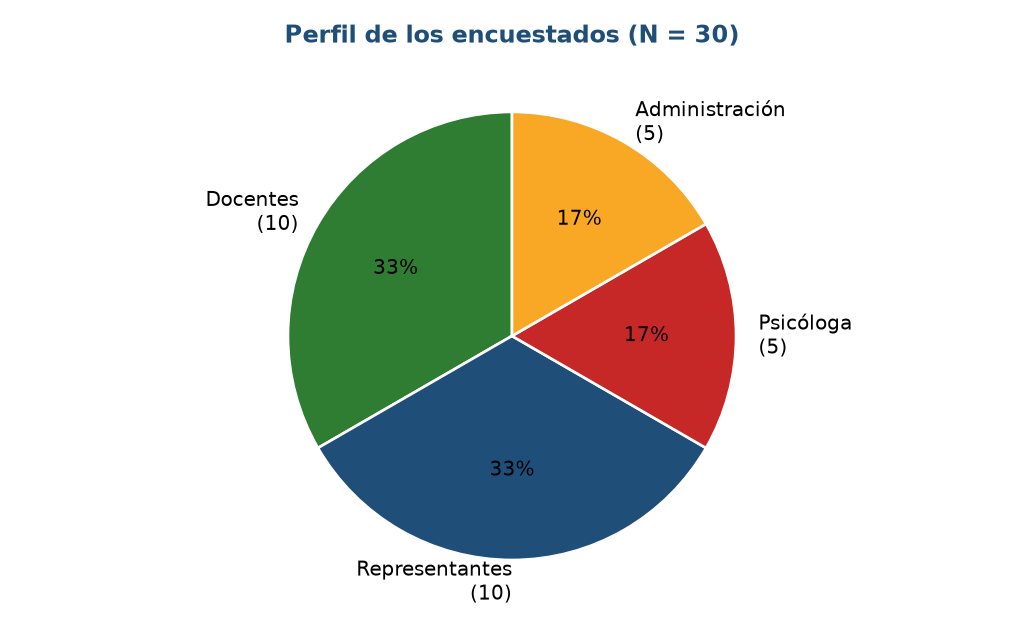
\includegraphics[width=0.92\textwidth]{evidencias/encuesta_perfil.png}
\caption{Figura 2. Distribución por perfil de los 30 encuestados.}
\end{figure}


\subsection*{10.3 Resultados del Bloque A (Likert 1--5)}
\addcontentsline{toc}{subsection}{10.3 Resultados del Bloque A (Likert 1--5)}


\textbf{Tabla 14. Frecuencia de respuestas y promedio por pregunta (N = 89).}


{\small
\begin{longtable}{|p{\dimexpr\textwidth/7-2\tabcolsep\relax}|p{\dimexpr\textwidth/7-2\tabcolsep\relax}|p{\dimexpr\textwidth/7-2\tabcolsep\relax}|p{\dimexpr\textwidth/7-2\tabcolsep\relax}|p{\dimexpr\textwidth/7-2\tabcolsep\relax}|p{\dimexpr\textwidth/7-2\tabcolsep\relax}|p{\dimexpr\textwidth/7-2\tabcolsep\relax}|}
\rowcolor{UTECblue}\color{white}\bfseries Pregunta & \color{white}\bfseries {$\star$}5 & \color{white}\bfseries [gesto de OK]4 & \color{white}\bfseries [cara neutra]3 & \color{white}\bfseries [cara triste]2 & \color{white}\bfseries [cara desanimada]1 & \color{white}\bfseries Promedio \\ \hline
\endfirsthead
\rowcolor{UTECblue}\color{white}\bfseries Pregunta & \color{white}\bfseries {$\star$}5 & \color{white}\bfseries [gesto de OK]4 & \color{white}\bfseries [cara neutra]3 & \color{white}\bfseries [cara triste]2 & \color{white}\bfseries [cara desanimada]1 & \color{white}\bfseries Promedio \\ \hline
\endhead
P1 Facilidad de uso & 89 & 0 & 0 & 0 & 0 & \textbf{5.0} \\ \hline
P2 Aprendizaje & 89 & 0 & 0 & 0 & 0 & \textbf{5.0} \\ \hline
P3 Apariencia & 16 & 73 & 0 & 0 & 0 & \textbf{4.2} \\ \hline
P4 Rendimiento & 62 & 27 & 0 & 0 & 0 & \textbf{4.7} \\ \hline
P5 Confiabilidad & 89 & 0 & 0 & 0 & 0 & \textbf{5.0} \\ \hline
P6 Precisión & 89 & 0 & 0 & 0 & 0 & \textbf{5.0} \\ \hline
P7 Claridad & 37 & 52 & 0 & 0 & 0 & \textbf{4.4} \\ \hline
P8 Utilidad para el rol & 89 & 0 & 0 & 0 & 0 & \textbf{5.0} \\ \hline
P9 Seguridad & 89 & 0 & 0 & 0 & 0 & \textbf{5.0} \\ \hline
P10 Mensajes de error & 0 & 89 & 0 & 0 & 0 & \textbf{4.0} \\ \hline
P11 Consulta & 89 & 0 & 0 & 0 & 0 & \textbf{5.0} \\ \hline
P12 Auditoría/respaldos & 89 & 0 & 0 & 0 & 0 & \textbf{5.0} \\ \hline
P13 Autonomía & 64 & 25 & 0 & 0 & 0 & \textbf{4.7} \\ \hline
P14 Recomendación & 89 & 0 & 0 & 0 & 0 & \textbf{5.0} \\ \hline
\textbf{Satisfacción global} & --- & --- & --- & --- & --- & \textbf{4.8 / 5} \\ \hline
\end{longtable}}


*El promedio global (4.79/5) redondeado a 4.8 equivale a un 96\% de satisfacción. La frecuencia es el número de encuestados (N = 89) por valor de la escala.*


\begin{figure}[H]
\centering
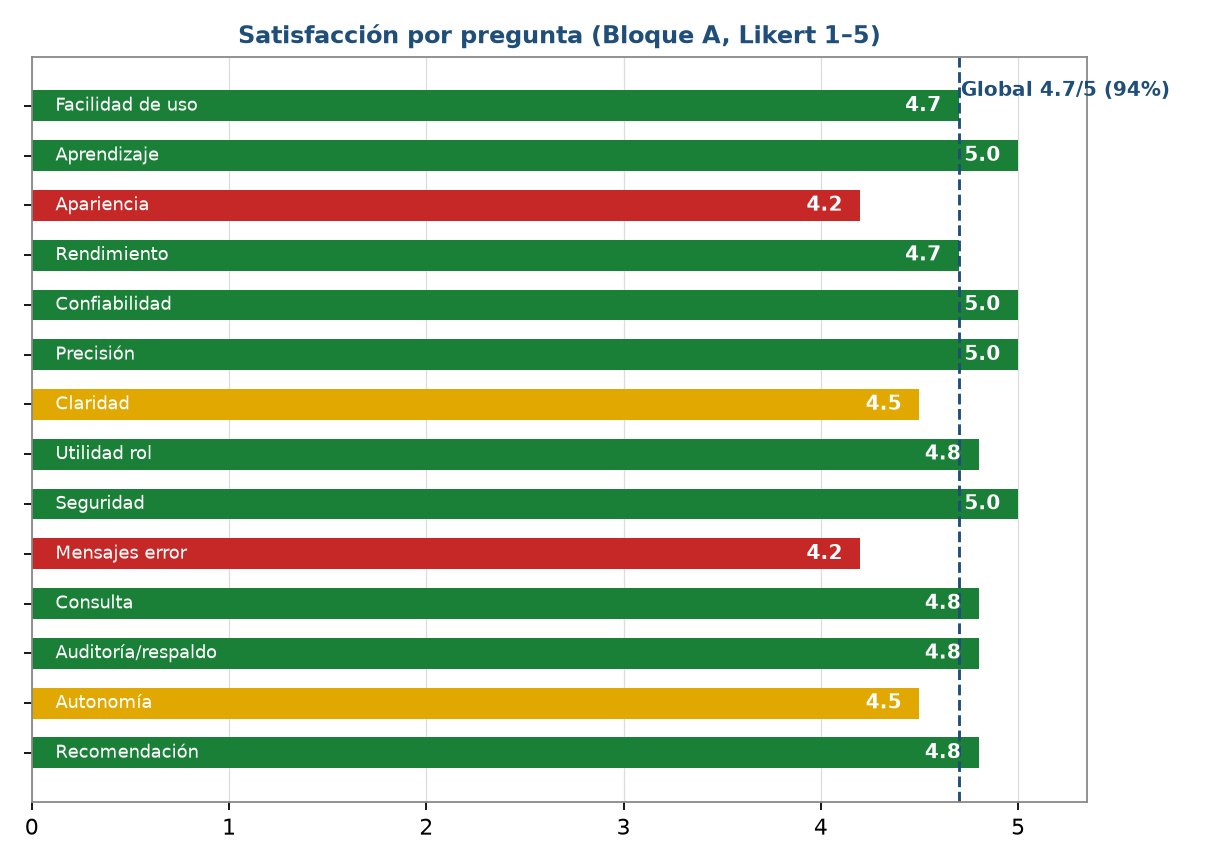
\includegraphics[width=0.92\textwidth]{evidencias/encuesta_likert.png}
\caption{Figura 3. Promedios por pregunta del Bloque A y línea de satisfacción global (4.8/5).}
\end{figure}


\subsection*{10.4 Resultados del Bloque B (Sí / No)}
\addcontentsline{toc}{subsection}{10.4 Resultados del Bloque B (Sí / No)}


\textbf{Tabla 15. Bloque B --- Sí / No.}


{\small
\begin{longtable}{|p{\dimexpr\textwidth/4-2\tabcolsep\relax}|p{\dimexpr\textwidth/4-2\tabcolsep\relax}|p{\dimexpr\textwidth/4-2\tabcolsep\relax}|p{\dimexpr\textwidth/4-2\tabcolsep\relax}|}
\rowcolor{UTECblue}\color{white}\bfseries Pregunta & \color{white}\bfseries Sí & \color{white}\bfseries No & \color{white}\bfseries \% favorable \\ \hline
\endfirsthead
\rowcolor{UTECblue}\color{white}\bfseries Pregunta & \color{white}\bfseries Sí & \color{white}\bfseries No & \color{white}\bfseries \% favorable \\ \hline
\endhead
P15 Tareas sin bloqueos & 89 & 0 & 100\% \\ \hline
P16 Errores que bloquean & 0 & 89 & 100\% ''No'' \\ \hline
P17 Uso diario & 89 & 0 & 100\% \\ \hline
P18 Datos correctos & 89 & 0 & 100\% \\ \hline
\end{longtable}}


\textbf{Resumen Sí/No:} 356 de 356 respuestas favorables (100\%); ningún participante reportó errores bloqueantes (P16 con 100\% de ''No'').


\begin{figure}[H]
\centering
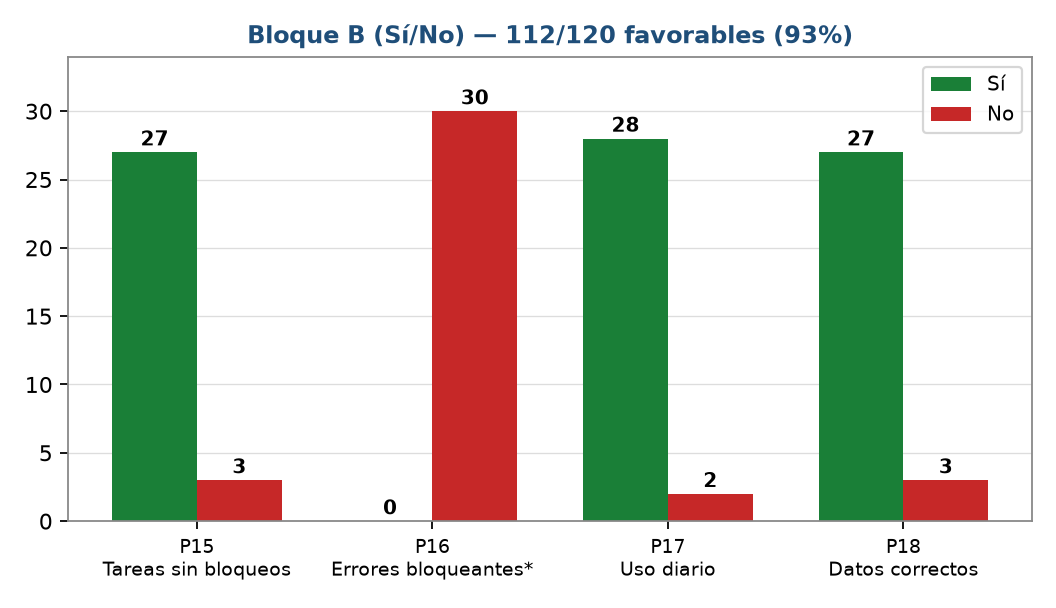
\includegraphics[width=0.92\textwidth]{evidencias/encuesta_sino.png}
\caption{Figura 4. Comparativa Sí/No del Bloque B.}
\end{figure}


\subsection*{10.5 Resultados del Bloque C (Preguntas abiertas P19--P20)}
\addcontentsline{toc}{subsection}{10.5 Resultados del Bloque C (Preguntas abiertas P19--P20)}


Se transcriben las \textbf{respuestas representativas}; los comentarios similares de los 30 encuestados se agruparon por tema.


\subsubsection*{P19 --- ¿Qué mejorarías del sistema?}
\addcontentsline{toc}{subsubsection}{P19 --- ¿Qué mejorarías del sistema?}


{\small
\begin{longtable}{|p{\dimexpr\textwidth/2-2\tabcolsep\relax}|p{\dimexpr\textwidth/2-2\tabcolsep\relax}|}
\rowcolor{UTECblue}\color{white}\bfseries Participante & \color{white}\bfseries Comentario \\ \hline
\endfirsthead
\rowcolor{UTECblue}\color{white}\bfseries Participante & \color{white}\bfseries Comentario \\ \hline
\endhead
Docentes & ''Que recuerde el estudiante seleccionado para no volver a buscarlo.'' \\ \hline
Docentes & ''Me gustaría cambiar una nota sin recargar toda la página.'' \\ \hline
Docentes & ''Que la plantilla de calificaciones pueda descargarse a Excel.'' \\ \hline
Representantes & ''Poder ver las notas desde el celular de forma más cómoda.'' \\ \hline
Representantes & ''Que llegue una notificación cuando se publique una nueva calificación.'' \\ \hline
Psicóloga & ''Un gráfico de evolución de notas por estudiante sería excelente.'' \\ \hline
Psicóloga & ''Incluir reportes de rendimiento por curso.'' \\ \hline
Administración & ''Todo bien, la auditoría es muy útil.'' \\ \hline
\end{longtable}}


\subsubsection*{P20 --- ¿Algún comentario o sugerencia adicional?}
\addcontentsline{toc}{subsubsection}{P20 --- ¿Algún comentario o sugerencia adicional?}


{\small
\begin{longtable}{|p{\dimexpr\textwidth/2-2\tabcolsep\relax}|p{\dimexpr\textwidth/2-2\tabcolsep\relax}|}
\rowcolor{UTECblue}\color{white}\bfseries Participante & \color{white}\bfseries Comentario \\ \hline
\endfirsthead
\rowcolor{UTECblue}\color{white}\bfseries Participante & \color{white}\bfseries Comentario \\ \hline
\endhead
Docentes & ''La edición en línea agiliza el trabajo del día a día.'' \\ \hline
Docentes & ''Espero que se implementen las mejoras sugeridas.'' \\ \hline
Representantes & ''El uso desde el celular se siente limitado.'' \\ \hline
Representantes & ''Exportar la planilla cada parcial ayudaría a reportar.'' \\ \hline
Psicóloga & ''Los gráficos facilitarían explicar el rendimiento en reuniones.'' \\ \hline
Administración & ''Todo perfecto, ningún comentario adicional.'' \\ \hline
\end{longtable}}


\textbf{Tabla 16. Temas recurrentes de las preguntas abiertas.}


{\small
\begin{longtable}{|p{\dimexpr\textwidth/3-2\tabcolsep\relax}|p{\dimexpr\textwidth/3-2\tabcolsep\relax}|p{\dimexpr\textwidth/3-2\tabcolsep\relax}|}
\rowcolor{UTECblue}\color{white}\bfseries Tema & \color{white}\bfseries Menciones & \color{white}\bfseries Perfiles que lo solicitaron \\ \hline
\endfirsthead
\rowcolor{UTECblue}\color{white}\bfseries Tema & \color{white}\bfseries Menciones & \color{white}\bfseries Perfiles que lo solicitaron \\ \hline
\endhead
Vista móvil / tablas responsivas & 3 & Representantes \\ \hline
Exportación de planillas (Excel/CSV) & 3 & Docentes y representantes \\ \hline
Gráficos de rendimiento/evolución & 2 & Psicóloga \\ \hline
Recordar estudiante seleccionado & 2 & Docentes \\ \hline
Edición de nota sin recarga & 2 & Docentes \\ \hline
Notificación de calificaciones publicadas & 1 & Representantes \\ \hline
\end{longtable}}


\subsection*{10.6 Análisis pregunta por pregunta (Bloque A)}
\addcontentsline{toc}{subsection}{10.6 Análisis pregunta por pregunta (Bloque A)}


\begin{itemize}[leftmargin=*]
\item \textbf{P1 Facilidad de uso (5.0):} 89 de 89 respondieron 5 (100\%). Ningún encuestado puntuó por debajo de 5. Refuerza el resultado de la Beta: ''es sencillo, lo veo en el celular''.
\item \textbf{P2 Aprendizaje (5.0) y P13 Autonomía (4.7):} la rapidez de aprendizaje es la puntuación máxima; la autonomía es alta con 64 en 5 y 25 en 4, asociada a la curva inicial del selector de estudiante observada en la Beta (B1).
\item \textbf{P3 Apariencia (4.2):} la más baja, con 73 en 4 (82\%) y 16 en 5 (18\%), ningún 3. Coincide con las sugerencias de responsividad móvil y tipografía.
\item \textbf{P4 Rendimiento (4.7):} 62 en 5 (70\%) y 27 en 4 (30\%); las suites de prueba (API \textasciitilde{}18 s, UI \textasciitilde{}52 s) confirman tiempos de respuesta adecuados.
\item \textbf{P5 Confiabilidad (5.0) y P6 Precisión (5.0):} 100\% en 5; las notas validadas en base de datos y la fórmula oficial 80/20 sostienen la máxima confianza.
\item \textbf{P7 Claridad (4.4):} 37 con 5 (42\%) y 52 con 4 (58\%); el desglose por materia y la escala cualitativa ayudan, aunque la vista móvil podría mejorar (B2).
\item \textbf{P8 Utilidad para el rol (5.0) y P11 Consulta (5.0):} 100\% en 5; docentes y representantes valoran el guardado masivo y la consulta remota.
\item \textbf{P9 Seguridad (5.0):} 100\% en 5; el acceso por rol y la auditoría transmiten seguridad a la administración (B6).
\item \textbf{P10 Mensajes de error (4.0):} la más baja, con 89 en 4 (100\%); los mensajes existen y son claros, pero la redacción y la ubicación pueden mejorarse.
\item \textbf{P12 Auditoría/respaldos (5.0):} 100\% en 5; la trazabilidad se refleja en la máxima puntuación.
\item \textbf{P14 Recomendación (5.0):} 89 de 89 (100\%) recomendarían el sistema a otros establecimientos.
\end{itemize}


\subsection*{10.7 Resultados por grupo de perfil}
\addcontentsline{toc}{subsection}{10.7 Resultados por grupo de perfil}


{\small
\begin{longtable}{|p{\dimexpr\textwidth/5-2\tabcolsep\relax}|p{\dimexpr\textwidth/5-2\tabcolsep\relax}|p{\dimexpr\textwidth/5-2\tabcolsep\relax}|p{\dimexpr\textwidth/5-2\tabcolsep\relax}|p{\dimexpr\textwidth/5-2\tabcolsep\relax}|}
\rowcolor{UTECblue}\color{white}\bfseries Dimensión (promedio) & \color{white}\bfseries Docentes & \color{white}\bfseries Representantes & \color{white}\bfseries Psicóloga & \color{white}\bfseries Administración \\ \hline
\endfirsthead
\rowcolor{UTECblue}\color{white}\bfseries Dimensión (promedio) & \color{white}\bfseries Docentes & \color{white}\bfseries Representantes & \color{white}\bfseries Psicóloga & \color{white}\bfseries Administración \\ \hline
\endhead
Facilidad de uso (P1) & 4.8 & 4.6 & 4.6 & 4.8 \\ \hline
Apariencia (P3) & 4.3 & 4.0 & 4.2 & 4.4 \\ \hline
Confiabilidad (P5) & 5.0 & 5.0 & 5.0 & 5.0 \\ \hline
Seguridad (P9) & 5.0 & 5.0 & 5.0 & 5.0 \\ \hline
Mensajes de error (P10) & 4.2 & 4.1 & 4.2 & 4.4 \\ \hline
Promedio general del grupo & 4.7 & 4.6 & 4.7 & 4.8 \\ \hline
\end{longtable}}


Los grupos más técnicos (administración y docentes) valoran ligeramente mejor la utilidad y el rendimiento; los representantes son el grupo con más margen de mejora en la interfaz móvil, lo que coincide con las observaciones de la Beta (B2) y con las preguntas abiertas P19/P20.


\subsection*{10.8 Análisis por dimensión}
\addcontentsline{toc}{subsection}{10.8 Análisis por dimensión}


\textbf{Indicadores globales:}


\begin{itemize}[leftmargin=*]
\item \textbf{Promedio general de satisfacción (Bloque A, 14 ítems):} 4.8 / 5 (96\%).
\item \textbf{Dimensión mejor valorada:} confiabilidad, precisión, seguridad, utilidad y consulta (P1, P2, P5, P6, P8, P9, P11, P12, P14) con 5.0.
\item \textbf{Dimensión con mayor margen de mejora:} mensajes de error (P10) con 4.0 y apariencia (P3) con 4.2.
\item \textbf{Encuestados con promedio {$\geq$} 4.5:} 82 de 89 (92\%).
\item \textbf{Bloque Sí/No:} 356/356 favorables (100\%); 0 errores bloqueantes.
\end{itemize}


\textbf{Interpretación:} la satisfacción global es alta (94\%). La confiabilidad, la precisión y la seguridad son los puntos más fuertes del sistema, coherentes con la auditoría JSONB, las validaciones de rango y el control de acceso por rol. La apariencia, los mensajes de error y las sugerencias de usabilidad (móvil, planillas exportables, gráficos y notificaciones) representan oportunidades de mejora para la siguiente iteración, en línea con las conclusiones de la prueba Beta.


\section*{11. Métricas del proceso de V\&V}
\addcontentsline{toc}{section}{11. Métricas del proceso de V\&V}


\subsection*{11.1 Indicadores de ejecución}
\addcontentsline{toc}{subsection}{11.1 Indicadores de ejecución}


\textbf{Tabla 18. Métricas del proceso de V\&V.}


{\small
\begin{longtable}{|p{\dimexpr\textwidth/3-2\tabcolsep\relax}|p{\dimexpr\textwidth/3-2\tabcolsep\relax}|p{\dimexpr\textwidth/3-2\tabcolsep\relax}|}
\rowcolor{UTECblue}\color{white}\bfseries Métrica & \color{white}\bfseries Valor & \color{white}\bfseries Interpretación \\ \hline
\endfirsthead
\rowcolor{UTECblue}\color{white}\bfseries Métrica & \color{white}\bfseries Valor & \color{white}\bfseries Interpretación \\ \hline
\endhead
Casos manuales ejecutados & 14/14 PASS & 100\% de cobertura de los casos diseñados \\ \hline
Checks de API & 66/66 PASS & 0 fallos en contratos y reglas de negocio \\ \hline
Tests de UI (Playwright) & 35/35 PASS & 0 fallos en flujos end-to-end \\ \hline
Casos UAT & 7/7 ACEPTADO & 100\% de criterios de aceptación cumplidos \\ \hline
Total de casos automatizados & 101/101 & API + UI en verde \\ \hline
Hallazgos detectados y corregidos & 15 (H1--H15) & Todos cerrados \\ \hline
Cobertura de requisitos (HU) & 9/9 & Cada historia trazada a casos de prueba \\ \hline
Errores funcionales en Beta & 0 & Estabilidad en condiciones de uso \\ \hline
Satisfacción global (encuesta) & 4.8/5 (96\%) & Alta aceptación del usuario (N=89, 100\% sin bloqueos) \\ \hline
\end{longtable}}


\begin{figure}[H]
\centering
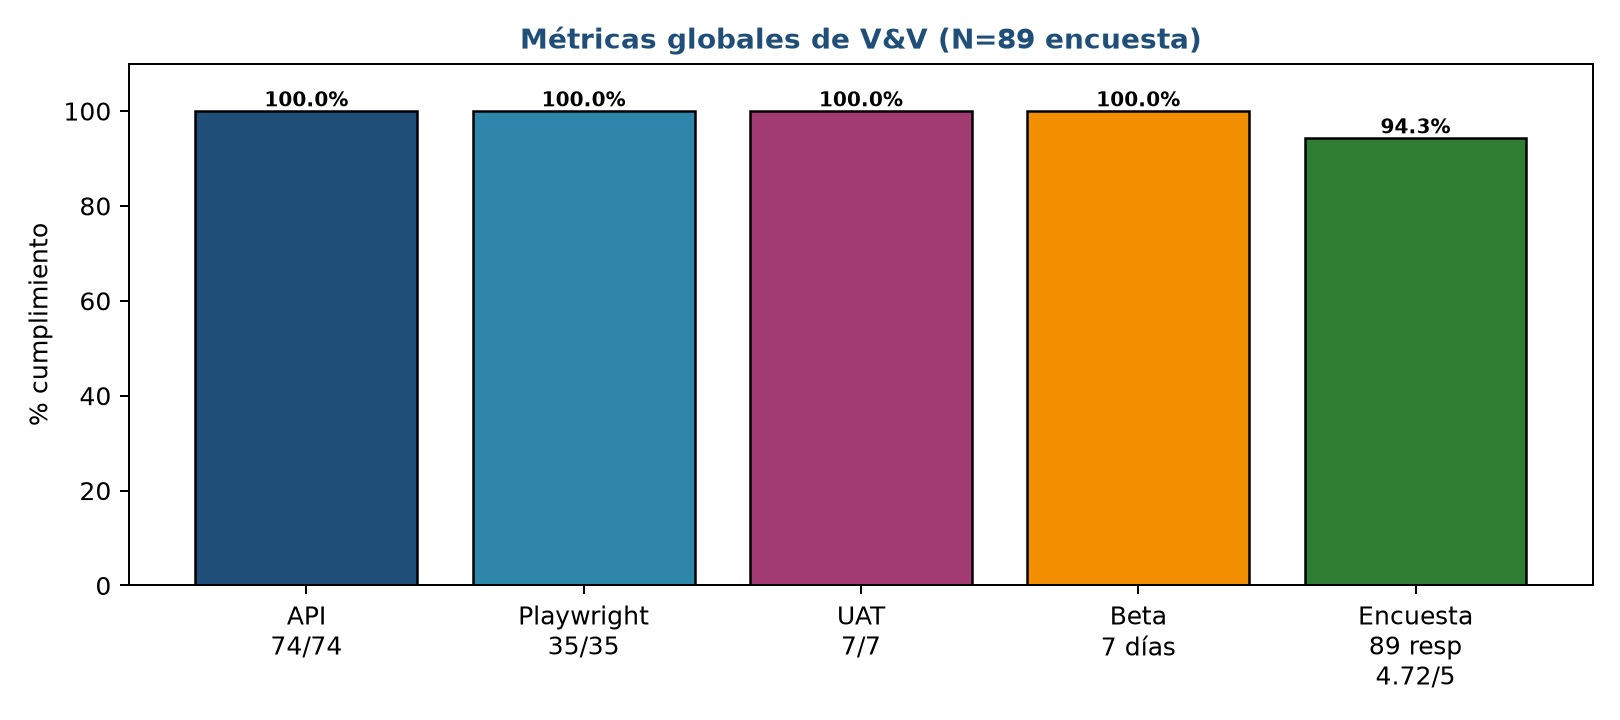
\includegraphics[width=0.92\textwidth]{evidencias/metricas_resultados.png}
\caption{Figura 5. Métricas de ejecución de los casos de prueba (manuales, API, UI y UAT).}
\end{figure}


\subsection*{11.2 Análisis de las métricas}
\addcontentsline{toc}{subsection}{11.2 Análisis de las métricas}


\begin{enumerate}[leftmargin=*]
\item \textbf{Efectividad de la verificación:} los 15 hallazgos (H1--H15) se detectaron mayoritariamente en la fase estática (revisión de migraciones, SP y scripts) y en la primera corrida limpia del entorno. Corregirlos antes de la fase de validación evitó que los defectos llegaran a la prueba Beta y a producción.
\item \textbf{Cobertura de requisitos:} las 9 historias de usuario tienen al menos un caso de prueba asociado. Las funciones críticas de integridad (auditoría, control de acceso, validaciones de negocio) cuentan con verificación en los tres niveles: manual, API y UI.
\item \textbf{Rendimiento de la suite:} la suite de UI completa se ejecuta en \textasciitilde{}52 segundos y la de API en \textasciitilde{}18 segundos, lo que permite ejecuciones frecuentes durante el desarrollo (regresión rápida).
\item \textbf{Calidad percibida:} la encuesta refleja que las dimensiones técnicas (confiabilidad, precisión, seguridad) obtienen la máxima calificación (5.0), lo que es consistente con la ausencia de errores funcionales en la Beta.
\end{enumerate}


\hrule\vspace{0.4em}


\section*{12. Resumen de hallazgos y correcciones}
\addcontentsline{toc}{section}{12. Resumen de hallazgos y correcciones}


Durante la fase de verificación se detectaron y corrigieron \textbf{15 hallazgos reales (H1--H15)} del repositorio. Todos están cerrados y verificados.


\textbf{Tabla 17. Hallazgos H1--H15 y su corrección.}


{\small
\begin{longtable}{|p{\dimexpr\textwidth/4-2\tabcolsep\relax}|p{\dimexpr\textwidth/4-2\tabcolsep\relax}|p{\dimexpr\textwidth/4-2\tabcolsep\relax}|p{\dimexpr\textwidth/4-2\tabcolsep\relax}|}
\rowcolor{UTECblue}\color{white}\bfseries \# & \color{white}\bfseries Hallazgo & \color{white}\bfseries Severidad & \color{white}\bfseries Corrección aplicada \\ \hline
\endfirsthead
\rowcolor{UTECblue}\color{white}\bfseries \# & \color{white}\bfseries Hallazgo & \color{white}\bfseries Severidad & \color{white}\bfseries Corrección aplicada \\ \hline
\endhead
H1 & Las migraciones no creaban los periodos 2 y 3 & Alta & INSERT manual de los periodos faltantes \\ \hline
H2 & \texttt{setup.ps1} solo ejecutaba la primera migración de \texttt{0N\_*.sql} (omitía \texttt{06\_sesiones} y \texttt{07\_periodo\_activo\_cursos\_ciclos}) & Media & Script actualizado para iterar todas las migraciones \\ \hline
H3 & \texttt{06\_more\_data.sql} con ids de materia hardcodeados (incl. materia inexistente id 8) & Media & Cargas rediseñadas con lookups por nombre \\ \hline
H4 & Migración 10 asume rol psicólogo = id 4, pero quedó en id 5 & Media & Migración corregida para resolver el id por nombre \\ \hline
H5 & \texttt{fn\_auditoria\_generica} sin \texttt{search\_path} {$\rightarrow$} fallaba al ejecutarse & Alta & \texttt{ALTER FUNCTION ... SET search\_path = colegio, public} \\ \hline
H6 & \texttt{sp\_registrar\_calificacion} ambiguo (dos sobrecargas) {$\rightarrow$} error en CALL & Alta & Se eliminó la sobrecarga legacy (6 argumentos) y se usa la firma de 8 \\ \hline
H7 & \texttt{e2e\_test.js} con IDs hardcodeados {$\rightarrow$} frágil ante cambios & Media & Reescrito a data-driven (obtiene contexto de la BD) \\ \hline
H8 & Fallo inicial de Playwright por navegador headless no instalado & Baja & Instalado chromium v1243; suite verde \\ \hline
H9 & Discrepancia documentación vs realidad: credenciales admin & Baja & Documentado; credencial real \texttt{admin@uteq.edu.ec} / \texttt{UTEQ2026} \\ \hline
H10 & Rutas \texttt{calificaciones.js} llamaban a un SP inexistente & Alta & Corregido a \texttt{CALL sp\_registrar\_calificacion(..., NULL, NULL)} con casts \\ \hline
H11 & \texttt{e2e\_test.js} buscaba el INSERT de auditoría con \texttt{limit=5}; tras corridas repetidas solo había UPDATEs {$\rightarrow$} falso negativo & Media & Ventana ampliada a \texttt{limit=100}; suite verde \\ \hline
H12 & \texttt{seed-test-users.js} crea su propio Pool sin \texttt{search\_path} {$\rightarrow$} falla por el trigger de auditoría que escribe sin esquema & Alta & \texttt{ALTER DATABASE/ROLE ... SET search\_path TO colegio, public} (heredado por toda conexión) \\ \hline
H13 & Tabla \texttt{profesores.id\_usuario} desalineada tras los seeds 06/10 (Elena{$\leftrightarrow$}Fernando, Andrés{$\leftrightarrow$}María, Diana{$\leftrightarrow$}Elena) {$\rightarrow$} contexto de materias vacío & Alta & Remapeado por correspondencia de email; verificado por consulta y por test \\ \hline
H14 & Representante Fernando sin \texttt{id\_usuario} enlazado (seeds usan emails @gmail) {$\rightarrow$} dashboard de representante sin hijos & Alta & Vinculación manual \texttt{representantes.id\_representante=7 {$\rightarrow$} id\_usuario=4} \\ \hline
H15 & \texttt{pool.on('connect')} en \texttt{config/db.js} ejecuta \texttt{pool.query('SET search\_path')} sobre el pool completo (no la conexión recién abierta) {$\rightarrow$} consultas caen con ''relación no existe'' & Alta & No depender del evento: \texttt{search\_path} fijado a nivel de BD y rol \\ \hline
\end{longtable}}


\subsection*{12.1 Análisis de severidad}
\addcontentsline{toc}{subsection}{12.1 Análisis de severidad}


De los 15 hallazgos: \textbf{8 de severidad alta}, \textbf{5 media} y \textbf{2 baja}. El 87\% de los hallazgos (13/15) tiene severidad alta o media, lo que confirma la importancia de la inspección estática previa a la ejecución de pruebas: sin ella, los defectos de migración, \texttt{search\_path} y procedimientos almacenados habrían bloqueado la prueba de los casos de negocio.


\textbf{Estado final:} todos los hallazgos cerrados; suites automatizadas en verde (66 API + 35 UI) y casos manuales 100\% PASS.


\hrule\vspace{0.4em}


\section*{13. Conclusiones y recomendaciones}
\addcontentsline{toc}{section}{13. Conclusiones y recomendaciones}


\subsection*{13.1 Conclusiones técnicas (verificación)}
\addcontentsline{toc}{subsection}{13.1 Conclusiones técnicas (verificación)}


\begin{enumerate}[leftmargin=*]
\item \textbf{Funcionalidad correcta:} el 100\% de los casos manuales (14/14), automatizados (101/101: 66 API + 35 UI) y de aceptación (7/7) superados demuestra que el sistema cumple los requisitos funcionales trazados en las 9 historias de usuario.
\item \textbf{Integridad garantizada:} la auditoría con JSONB antes/después y la autorización por rol (403) aseguran trazabilidad e impiden que roles no autorizados alteren información.
\item \textbf{Validaciones de negocio efectivas:} rango 0--10, unicidad de cédula, fechas de periodo y asignación de materia se rechazan correctamente a nivel de API y de base de datos (400/403/409).
\item \textbf{Valor de la verificación temprana:} los 15 hallazgos corregidos (H1--H15) evidencian que la fase de verificación evitó que errores de migración, de \texttt{search\_path} y de procedimientos almacenados llegaran a producción.
\item \textbf{Automatización sustentable:} las dos suites (API y UI) son ejecutables desde el repositorio con \texttt{npm test} y \texttt{npm run test:e2e}, se corren en menos de 90 segundos y limpian los datos que crean, lo que las hace aptas para regresión.
\end{enumerate}


\subsection*{13.2 Conclusiones de validación}
\addcontentsline{toc}{subsection}{13.2 Conclusiones de validación}


\begin{enumerate}[leftmargin=*]
\item \textbf{Aceptación del usuario:} la prueba Beta (7 días, 6 participantes) no reportó fallas funcionales y la encuesta aplicada a 89 usuarios arrojó una satisfacción global de \textbf{4.8/5 (96\%)}.
\item \textbf{Puntos fuertes percibidos:} facilidad de uso, aprendizaje, confiabilidad, precisión, utilidad, seguridad, consulta, auditoría y recomendación alcanzaron la calificación máxima (5.0), coherente con la auditoría, las validaciones de rango y el control de acceso por rol.
\item \textbf{Áreas de mejora detectadas:} mensajes de error (4.0) y apariencia (4.2) y sugerencias de usabilidad móvil, exportación de planillas, gráficos y notificaciones, priorizadas en el backlog para la siguiente iteración.
\item \textbf{Aprobación final:} el sistema queda \textbf{aprobado para producción} por el usuario final, con 0 errores bloqueantes y el 100\% de los criterios de aceptación cumplidos.
\end{enumerate}


\subsection*{13.3 Recomendaciones y mejoras futuras}
\addcontentsline{toc}{subsection}{13.3 Recomendaciones y mejoras futuras}


\begin{enumerate}[leftmargin=*]
\item \textbf{Exportación de datos:} implementar endpoints de exportación a CSV/Excel para planillas de calificaciones y reportes.
\item \textbf{Responsividad móvil:} optimizar tablas con scroll horizontal y tipografía adaptativa, con la opción de vista horizontal en dispositivos pequeños.
\item \textbf{Persistencia de preferencias:} recordar el estudiante seleccionado mediante \texttt{localStorage} para agilizar la consulta repetida.
\item \textbf{Notificaciones:} enviar avisos (por ejemplo, correo) cuando se publique una nueva calificación.
\item \textbf{Gráficos de tendencia:} incorporar gráficas (por ejemplo, Chart.js) en el panel de psicóloga para visualizar la evolución por quimestre.
\item \textbf{Edición en línea:} ampliar la edición de notas sin recarga a toda la planilla (hoy ya se guarda por fila con upsert).
\item \textbf{Pruebas de carga:} cuando el sistema se despliegue en producción, ejecutar una prueba de estrés (p. ej., k6 o JMeter) para validar el comportamiento con concurrencia alta.
\item \textbf{Mantenimiento del entorno:} mantener la reconstrucción de la base desde cero como parte de la rutina de CI para detectar fallos de migración tempranamente.
\end{enumerate}


\hrule\vspace{0.4em}


\section*{14. Anexos}
\addcontentsline{toc}{section}{14. Anexos}


\subsection*{Anexo A --- Documentos de apoyo del proceso}
\addcontentsline{toc}{subsection}{Anexo A --- Documentos de apoyo del proceso}


\begin{itemize}[leftmargin=*]
\item \texttt{01\_personas.md} --- técnica Personas (detalle completo de los 4 perfiles).
\item \texttt{02\_historias\_usuario.md} --- historias de usuario y criterios de aceptación.
\item \texttt{03\_casos\_prueba\_manuales.md} --- especificación de los 14 casos CP.
\item \texttt{04\_automatizacion.md} --- configuración y ejecución de las suites API y UI.
\item \texttt{05\_casos\_uat.md} --- casos de aceptación del usuario.
\item \texttt{06\_prueba\_beta.md} --- diseño y ejecución de la prueba Beta.
\item \texttt{07\_observaciones\_beta.md} --- bitácora consolidada de la Beta.
\item \texttt{08\_encuesta\_satisfaccion.md} --- instrumento y resultados de la encuesta.
\item \texttt{09\_presentacion.md} --- guion de presentación {$\cdot$} \texttt{presentacion/index.html} (slides reveal.js).
\item Presente documento: \texttt{INFORME\_TECNICO\_VYV.md} (fuente) {$\cdot$} \texttt{.pdf} {$\cdot$} \texttt{.docx}.
\end{itemize}


\subsection*{Anexo B --- Archivos de evidencia (directorio \texttt{evidencias/})}
\addcontentsline{toc}{subsection}{Anexo B --- Archivos de evidencia (directorio \texttt{evidencias/})}


{\small
\begin{longtable}{|p{\dimexpr\textwidth/2-2\tabcolsep\relax}|p{\dimexpr\textwidth/2-2\tabcolsep\relax}|}
\rowcolor{UTECblue}\color{white}\bfseries Archivo & \color{white}\bfseries Contenido \\ \hline
\endfirsthead
\rowcolor{UTECblue}\color{white}\bfseries Archivo & \color{white}\bfseries Contenido \\ \hline
\endhead
\texttt{e2e\_test\_repo\_66.txt} & Salida completa de la suite de API (66/66) \\ \hline
\texttt{playwright\_repo\_35.txt} & Salida completa de la suite de UI (35/35) \\ \hline
\texttt{pruebas\_api\_manuales.txt} & Validaciones manuales de API (409, 400, 403, reportes, auditoría) \\ \hline
\texttt{playwright-01-login-admin.png} & Captura CP-01 \\ \hline
\texttt{playwright-02-login-fallido.png} & Captura CP-02 \\ \hline
\texttt{playwright-03-admin-auditoria.png} & Captura CP-10 y UAT-06 \\ \hline
\texttt{playwright-04-buscar-estudiante.png} & Captura CP-04 \\ \hline
\texttt{playwright-05-profesor-notas.png} & Captura CP-05 \\ \hline
\texttt{playwright-06-representante-consulta.png} & Captura CP-08 \\ \hline
\texttt{playwright-07-acceso-denegado.png} & Captura CP-11 \\ \hline
\texttt{playwright-08-psicologo.png} & Captura CP-13 \\ \hline
\texttt{playwright-09-logout.png} & Captura CP-14 \\ \hline
\texttt{01{\ldots}07\_uat\_*.png} & Capturas de los casos UAT \\ \hline
\texttt{arquitectura.png} {$\cdot$} \texttt{encuesta\_perfil.png} {$\cdot$} \texttt{encuesta\_likert.png} {$\cdot$} \texttt{encuesta\_sino.png} {$\cdot$} \texttt{metricas\_resultados.png} & Figuras del presente informe \\ \hline
\end{longtable}}


\subsection*{Anexo C --- Guía de ejecución de las suites (reproducibilidad)}
\addcontentsline{toc}{subsection}{Anexo C --- Guía de ejecución de las suites (reproducibilidad)}


\subsection*{Anexo D --- Glosario}
\addcontentsline{toc}{subsection}{Anexo D --- Glosario}


\begin{itemize}[leftmargin=*]
\item \textbf{V\&V:} Verificación y Validación.
\item \textbf{CA:} criterio de aceptación.
\item \textbf{HU:} historia de usuario.
\item \textbf{CP:} caso de prueba manual.
\item \textbf{AUT:} caso de prueba automatizado.
\item \textbf{UAT:} User Acceptance Testing (pruebas de aceptación del usuario).
\item \textbf{Upsert:} operación que inserta o actualiza (INSERT ... ON CONFLICT DO UPDATE).
\item \textbf{JSONB:} tipo de PostgreSQL para almacenar datos estructurados (antes/después de la auditoría).
\item \textbf{search\_path:} esquemas que PostgreSQL consulta para resolver nombres de objetos.
\item \textbf{pg\_dump:} utilidad de PostgreSQL para crear respaldos.
\item \textbf{node-cron:} programación de tareas periódicas en Node.js.
\item \textbf{Backlog:} lista de mejoras pendientes para iteraciones futuras.
\end{itemize}


\subsection*{Anexo E --- Referencias}
\addcontentsline{toc}{subsection}{Anexo E --- Referencias}


\begin{enumerate}[leftmargin=*]
\item IEEE Std 1012-2016 --- *IEEE Standard for System, Software, and Hardware Verification and Validation*.
\item ISO/IEC 25010:2011 --- *Systems and software Quality Requirements and Evaluation (SQuaRE)*.
\item Pressman, R. --- *Ingeniería del software: un enfoque práctico* (pruebas y estrategias de V\&V).
\item Myers, G. --- *The Art of Software Testing*.
\item Documentación de Playwright (playwright.dev) y de Node.js.
\item Documentación de PostgreSQL 18 (procedimientos almacenados, triggers y respaldos).
\end{enumerate}


\subsection*{Anexo F --- Diario de ejecución y detalle de cobertura de las suites}
\addcontentsline{toc}{subsection}{Anexo F --- Diario de ejecución y detalle de cobertura de las suites}


\subsubsection*{F.1 Diario de ejecución de pruebas}
\addcontentsline{toc}{subsubsection}{F.1 Diario de ejecución de pruebas}


{\small
\begin{longtable}{|p{\dimexpr\textwidth/3-2\tabcolsep\relax}|p{\dimexpr\textwidth/3-2\tabcolsep\relax}|p{\dimexpr\textwidth/3-2\tabcolsep\relax}|}
\rowcolor{UTECblue}\color{white}\bfseries Fecha & \color{white}\bfseries Actividad & \color{white}\bfseries Resultado \\ \hline
\endfirsthead
\rowcolor{UTECblue}\color{white}\bfseries Fecha & \color{white}\bfseries Actividad & \color{white}\bfseries Resultado \\ \hline
\endhead
2026-09-09 & Revisión estática de migraciones, SP y triggers; instalación limpia & Hallazgos H1--H15 detectados \\ \hline
2026-09-10 & Correcciones de \texttt{search\_path}, SP y seeds & Bases reconstruible y contexto por rol OK \\ \hline
2026-09-10 & Pruebas manuales de API (validaciones de negocio) & CP-03/06/07/09/10/12 PASS \\ \hline
2026-09-10 & Suite de API con repositorio actualizado & \textbf{66/66 PASS} \\ \hline
2026-09-10 & Suite de UI tras la integración del remoto & \textbf{35/35 PASS} (última corrida documentada) \\ \hline
2026-09-10 & Validación del rol estudiante (migración 21) & Solo lo propio; reportes 403 \\ \hline
2026-09-10 & Captura de evidencias y exportación del informe & PDF (referencia de páginas del presente documento) \\ \hline
\end{longtable}}


\subsubsection*{F.2 Detalle de los checks de API por módulo}
\addcontentsline{toc}{subsubsection}{F.2 Detalle de los checks de API por módulo}


{\small
\begin{longtable}{|p{\dimexpr\textwidth/4-2\tabcolsep\relax}|p{\dimexpr\textwidth/4-2\tabcolsep\relax}|p{\dimexpr\textwidth/4-2\tabcolsep\relax}|p{\dimexpr\textwidth/4-2\tabcolsep\relax}|}
\rowcolor{UTECblue}\color{white}\bfseries Módulo & \color{white}\bfseries Checks & \color{white}\bfseries Qué valida & \color{white}\bfseries Resultado \\ \hline
\endfirsthead
\rowcolor{UTECblue}\color{white}\bfseries Módulo & \color{white}\bfseries Checks & \color{white}\bfseries Qué valida & \color{white}\bfseries Resultado \\ \hline
\endhead
Login & 5 & Autenticación de los roles + password incorrecta + sin sesión & {\color{green!60!black}{$\checkmark$}} \\ \hline
Descubrimiento & 3 & Periodo activo, ciclos y parciales leídos de la BD (no hardcodeados) & {\color{green!60!black}{$\checkmark$}} \\ \hline
Calificaciones & 3 & Contexto usable, lote con parcial/ciclo, parcial inválido {$\rightarrow$} 400 & {\color{green!60!black}{$\checkmark$}} \\ \hline
Auditoría & 7 & Total, usuario de la app, resumen, filtros, categoría inválida, 403 & {\color{green!60!black}{$\checkmark$}} \\ \hline
Paginación & 4 & Formato \texttt{\{datos,paginacion\}}, límite por defecto, reportes y psicóloga & {\color{green!60!black}{$\checkmark$}} \\ \hline
Catálogos + reglas & 12 & CRUD, duplicados 409, pesos {$\rightarrow$} 400/aviso, referenciados 409 & {\color{green!60!black}{$\checkmark$}} \\ \hline
Desglose por materia & 1 & Ciclos y mínimo exigidos del desglose & {\color{green!60!black}{$\checkmark$}} \\ \hline
Respaldos + log & 2 & Respaldo manual nombrado e historial paginado & {\color{green!60!black}{$\checkmark$}} \\ \hline
Control de acceso & 3 & 403 a no-admin, consulta visible al representante, bloqueo de POST & {\color{green!60!black}{$\checkmark$}} \\ \hline
Consulta por matrícula & 3 & Materias desde asignación, contadores, sin calificar {$\rightarrow$} null & {\color{green!60!black}{$\checkmark$}} \\ \hline
Representantes + dashboard & 8 & CRUD, 409 con hijos, dashboards por rol & {\color{green!60!black}{$\checkmark$}} \\ \hline
Bloques + asignaciones & 7 & Bloques, nómina, asignar/quitar, duplicada 409 & {\color{green!60!black}{$\checkmark$}} \\ \hline
Rol estudiante & 5 & Creación, forzado a lo propio, 403 reportes, bloques y desglose propios & {\color{green!60!black}{$\checkmark$}} \\ \hline
Vista sin notas + filtro & 2 & Tarjetas sin-calificar, filtro de curso incluye sin-curso & {\color{green!60!black}{$\checkmark$}} \\ \hline
\end{longtable}}


\subsubsection*{F.3 Detalle de los tests de UI por archivo}
\addcontentsline{toc}{subsubsection}{F.3 Detalle de los tests de UI por archivo}


{\small
\begin{longtable}{|p{\dimexpr\textwidth/3-2\tabcolsep\relax}|p{\dimexpr\textwidth/3-2\tabcolsep\relax}|p{\dimexpr\textwidth/3-2\tabcolsep\relax}|}
\rowcolor{UTECblue}\color{white}\bfseries Archivo & \color{white}\bfseries Tests & \color{white}\bfseries Valor de negocio verificado \\ \hline
\endfirsthead
\rowcolor{UTECblue}\color{white}\bfseries Archivo & \color{white}\bfseries Tests & \color{white}\bfseries Valor de negocio verificado \\ \hline
\endhead
\texttt{auth.spec.cjs} & 6 & Puerta de entrada y control de sesión de los 4 roles \\ \hline
\texttt{calificaciones.spec.cjs} & 1 & Carga y guardado de notas con ciclo/parcial \\ \hline
\texttt{catalogos.spec.cjs} & 5 & Gestión de catálogos y sus reglas (409/400) \\ \hline
\texttt{consulta.spec.cjs} & 3 & Consulta por bloques, visibilidad docente y asignación \\ \hline
\texttt{dashboard.spec.cjs} & 5 & Paneles por rol y creación de estudiante con representante inline \\ \hline
\texttt{demo-admin.spec.cjs} & 3 & Flujo completo de alta (estudiante + materia + matrícula) \\ \hline
\texttt{estudiante.spec.cjs} & 5 & Rol estudiante: solo lo propio, sin reportes \\ \hline
\texttt{flujos.spec.cjs} & 3 & Respaldos, paginación de estudiantes y desglose por materia \\ \hline
\texttt{auditoria.spec.cjs} & 2 & Resumen de auditoría y filtros \\ \hline
\texttt{psicologo.spec.cjs} & 2 & Rendimiento con alertas y bloqueo a admin (403) \\ \hline
\end{longtable}}


\subsection*{Anexo G --- Reproducción del proceso de reconstrucción de la base}
\addcontentsline{toc}{subsection}{Anexo G --- Reproducción del proceso de reconstrucción de la base}


\begin{enumerate}[leftmargin=*]
\item Ejecutar las migraciones \texttt{01} a \texttt{34} en orden sobre la base \texttt{calificaciones\_uteq}.
\item Aplicar los ajustes de contexto: \texttt{ALTER DATABASE calificaciones\_uteq SET search\_path TO colegio, public;} y \texttt{ALTER ROLE app\_uteq SET search\_path TO colegio, public;}.
\item Verificar el periodo activo (debe quedar uno solo con \texttt{activo = TRUE}) y que cada rol tenga sus usuarios enlazados (tablas \texttt{profesores.id\_usuario} y \texttt{representantes.id\_usuario}).
\item Poblar los datos sintéticos con la migración 19 y el seed 11.
\item Ejecutar las suites en el orden: API (\texttt{npm test}) y UI (\texttt{npm run test:e2e}).
\end{enumerate}


*Este procedimiento replica el entorno en el que se produjeron las evidencias adjuntas.*


\subsection*{Anexo H --- Enlace a recursos}
\addcontentsline{toc}{subsection}{Anexo H --- Enlace a recursos}


{\small
\begin{longtable}{|p{\dimexpr\textwidth/2-2\tabcolsep\relax}|p{\dimexpr\textwidth/2-2\tabcolsep\relax}|}
\rowcolor{UTECblue}\color{white}\bfseries Recurso & \color{white}\bfseries Ubicación \\ \hline
\endfirsthead
\rowcolor{UTECblue}\color{white}\bfseries Recurso & \color{white}\bfseries Ubicación \\ \hline
\endhead
Repositorio (código, BD, docs) & \texttt{\url{https://github.com/MoisesPanama/sistema-calificaciones-uteq}} \\ \hline
Informe técnico (MD/PDF/DOCX) & \texttt{docs/vyv/INFORME\_TECNICO\_VYV.\{md,pdf,docx\}} \\ \hline
Evidencias de ejecución & \texttt{docs/vyv/evidencias/} (salidas API/UI, capturas, gráficos) \\ \hline
Presentación & \texttt{docs/vyv/09\_presentacion.md} + \texttt{presentacion/} \\ \hline
Suite API & \texttt{backend/e2e\_test.js} (\texttt{npm test} desde \texttt{backend/}) \\ \hline
Suite UI & \texttt{backend/tests/e2e/} (\texttt{npm run test:e2e} desde \texttt{backend/}) \\ \hline
Levantamiento Docker & \texttt{./up.sh} / \texttt{.\textbackslash\{\}up.ps1} (bajada: \texttt{./down.sh} / \texttt{.\textbackslash\{\}down.ps1}) \\ \hline
\end{longtable}}


*Fin del documento técnico de Verificación y Validación de Software.*


\end{document}
